\documentclass[11pt,a4paper]{article}

\usepackage[utf8]{inputenc}
\usepackage[T1]{fontenc}
\usepackage{lmodern}
\usepackage{amsmath, amssymb, amsthm}
\usepackage{booktabs}
\usepackage{tabularx}
\usepackage{geometry}
\geometry{margin=1in}
\usepackage{microtype}
\usepackage{graphicx}
\usepackage{xcolor}
\definecolor{linknavy}{RGB}{0, 70, 130}
\usepackage{hyperref}
\hypersetup{colorlinks=true, linkcolor=linknavy, citecolor=linknavy, urlcolor=linknavy, breaklinks=true,
  pdftitle={Causal Inference for Compliance-Gated Administrative Data: A Tested Data-Generating Process Approach with Application to Municipal Energy Benchmarking},
  pdfauthor={Xuân Chính Mai}}
\usepackage{enumitem}
\usepackage{needspace}
\usepackage{placeins}
\usepackage{float}
\usepackage{longtable}
% Publication-quality figure captions: small text, 10 pt vertical skip.
% \caption*{} (starred) suppresses the automatic "Figure X." prefix so the
% manual "\textbf{Figure X.Y.} ..." embedded in each caption drives the label.
% singlelinecheck=false prevents single-line captions from being centred.
\usepackage[font=small,skip=10pt,justification=justified,
            singlelinecheck=false]{caption}

% Classic journal paragraph style: indented first lines, no inter-paragraph
% gap. (The draft renders previously used parskip's block paragraphs.)
\setlength{\parindent}{15pt}
\setlength{\parskip}{0pt plus 1pt}

% Keep paragraph-opening and -closing lines attached to their paragraph
% across page breaks (no widows/orphans in a submission-ready manuscript).
\widowpenalty=10000
\clubpenalty=10000

% Float placement: topfraction=0.72 means one wide figure + caption can sit
% at the top of a page (most figures are 200--400 pt scaled) but two cannot
% stack and cause overfull vboxes. floatpagefraction=0.65 is low enough that
% medium-tall figures (shap_combined ~514 pt, type_intercepts ~491 pt) reach
% a dedicated float page rather than being deferred to the document end.
% A \FloatBarrier is emitted at each \section{} boundary (not subsections) so
% figures stay inside their own section without creating mid-section gaps.
\renewcommand{\topfraction}{0.72}
\renewcommand{\bottomfraction}{0.60}
\renewcommand{\textfraction}{0.12}
\renewcommand{\floatpagefraction}{0.65}
\setcounter{topnumber}{2}
\setcounter{bottomnumber}{1}
\setcounter{totalnumber}{3}

% Top-align dedicated float pages: pack figures from the top and let any
% leftover space collect at the bottom, instead of spreading gaps between them.
\makeatletter
\setlength{\@fptop}{0pt}
\setlength{\@fpsep}{14pt plus 0fil}
\setlength{\@fpbot}{0pt plus 1fil}
\makeatother

\definecolor{citecolor}{RGB}{0, 90, 156}
\newcommand{\cit}[2]{\hyperlink{#1}{\textcolor{citecolor}{#2}}}

% Inline code: monospace with light gray background, mimicking Markdown rendering.
\newcommand{\code}[1]{{\setlength{\fboxsep}{2pt}\colorbox{gray!12}{\strut\texttt{#1}}}}

\newtheorem{definition}{Definition}[section]
\newtheorem{proposition}{Proposition}[section]

\title{Causal Inference for Compliance-Gated Administrative Data:\\
A Tested Data-Generating Process Approach with Application to Municipal Energy Benchmarking\thanks{Working paper, June 2026. This is a preprint circulated for discussion; comments are welcome. The analysis code, and the scripts that fetch the data and reproduce every figure and table, are openly available at \url{https://github.com/ChinhMaiGit/tdgp}.}}
\author{Xuân Chính Mai\\[2pt]
{\small Independent Researcher}\\[2pt]
{\small\texttt{chinhmai.work@gmail.com}}\\[2pt]
{\small ORCID: \href{https://orcid.org/0009-0000-7102-9546}{0009-0000-7102-9546}}}
\date{June 2026}

\begin{document}
\maketitle

% Loose typesetting for draft renders -- allow longer inter-word spaces to
% avoid overfull boxes on long math expressions and URLs.
\sloppy

\begin{abstract}
\noindent Every causal conclusion drawn from observational data is conditional on a causal graph, and in most applied work the graph is asserted rather than tested. This paper identifies a class of administrative datasets for which the testing problem is tractable: compliance-gated datasets, in which units report outcomes if and only if observable characteristics cross a regulatory threshold, so that the institutional documents defining the reporting obligation also encode the process that generated the data. We develop a three-stage pipeline, the Tested Data-Generating Process (TDGP), that locates the compliance gate in the dataset's missingness structure, formulates a candidate causal graph from that structure and the variable descriptions alone, and then tests the candidate against the constitutive documents, which are quarantined until the test. We demonstrate the pipeline on the Chicago Energy Benchmarking dataset, 28,329 building-year records (2014--2023) gated at 50,000 square feet, where the candidate survives the documentary test and the recorded data reproduce the EPA greenhouse-gas accounting identity to $R^2 = 0.9999$. A 2$\times$3 factorial experiment crossing causal correction with functional form then shows what the tested structure licenses: an inverse-probability-weighted hierarchical Bayesian model and IPW XGBoost converge to within 0.4 percentage points of median absolute percentage error (21.4\% against 21.0\%), evidence that structural and algorithmic models estimate the same causal quantity once the data-generating process is tested, and a resolution of Breiman's two-cultures tension under that condition. The tested structure further supports deployment prediction for the 5,510 non-compliant records excluded from all training and counterfactual policy queries that the gated sample alone cannot answer.
\par\bigskip\noindent\textbf{Keywords:} \textit{causal inference; directed acyclic graphs; selection bias; missing data; inverse probability weighting; energy benchmarking}
\end{abstract}

\section{Introduction}
Mandatory reporting programmes are widespread, and the administrative datasets they generate have become primary sources for empirical research in energy policy, environmental economics, public health, labour economics, and related fields (\cit{liangzhang2026}{Liang \& Zhang, 2026}). Such administrative data is increasingly recognised as a distinctive resource for social science, prized for its scale and population coverage but carrying selection and data-quality challenges that demand explicit methodological treatment (\cit{connellyetal2016}{Connelly et al., 2016}). The U.S. Securities and Exchange Commission requires publicly traded firms to file annual financial disclosures on Form 10-K via the EDGAR system (\cit{securitiesnd}{U.S. Securities and Exchange Commission, n.d.}). The Occupational Safety and Health Administration mandates injury and illness recordkeeping for entities above explicit employee-size thresholds, and requires larger establishments to submit these records electronically (\cit{departmentnd}{U.S. Department of Labor, Occupational Safety and Health Administration, n.d.}). The Environmental Protection Agency's Toxics Release Inventory requires annual reporting of chemical releases and waste management from facilities that meet industry, employment, and chemical-volume thresholds (\cit{environmentalnd}{U.S. Environmental Protection Agency, n.d.}). Numerous municipal and state energy benchmarking ordinances compel building owners to report annual energy consumption, applying to buildings that typically exceed 25,000--50,000 gross square feet (\cit{mengetal2017}{Meng et al., 2017}). In each case, the reporting obligation is triggered by an observable, verifiable characteristic of the reporting unit: firm size, establishment headcount, production or chemical-use volume, or building floor area. This design reflects a regulatory balance between compliance costs and informational benefits.

These programmes share a structural feature that is rarely made explicit: the observable characteristic that triggers the reporting obligation is also a causal determinant of the outcome variable that researchers typically study. A large office building, for example, must report its energy use precisely because it is large, and it emits substantially more greenhouse gases because it is large. Consequently, the compliance threshold does not select units into the observed sample at random. Instead, it systematically enriches the sample with units that exhibit the highest values of the outcome variable. This is not random missingness or dropout; it is systematic unit-level selection on a variable that is simultaneously the selection criterion and a cause of the outcome (\cit{hernanrobins2020}{Hernán \& Robins, 2020, Chapter 8}).

Standard analyses do not correct for this selection mechanism. Regression, gradient-boosted trees, and Bayesian models alike treat the observed sample as representative of the target population unless a correction is added explicitly, and none of the standard modelling pipelines includes one by default. A model fitted to the observed sample estimates the outcome distribution conditional on compliance, P(Y | X, C = 1), when the question of interest is the population relationship P(Y | X). The two quantities differ whenever compliance C is endogenous to the predictors X. This is not a limitation of predictive modelling that can be overcome with more flexible algorithms or more data. It is a causal inference problem: because the sampling mechanism is endogenous to the predictors, associational approaches cannot recover the target population relationship without an explicit model of the selection process.

\cit{pearl2018}{Pearl (2018)} states the underlying limitation directly: no volume of data can answer a causal question without a model of the process that generated it. The failure of conventional workflows is therefore invisible from within those workflows. Cross-validation accuracy does not reveal the bias, because the held-out test set is drawn from the same compliance-enriched distribution as the training set; the model is evaluated against the very population it was fitted to. As a result, high predictive performance on observed data can coexist with systematic distortion of the population-level relationships that researchers and policymakers actually wish to understand.

The ingredients of a solution exist across separate literatures, yet no widely adopted procedure currently integrates them for compliance-gated administrative data. \cit{pearl2019}{Pearl (2019)} identifies seven foundational tools of causal inference and emphasises that causal structure must precede data analysis. However, this framework remains conceptual and does not provide a concrete procedure for recovering that structure from a specific administrative dataset. The causal inference literature offers inverse probability weighting (IPW) as a standard correction for selection bias (\cit{hernanrobins2020}{Hernán \& Robins, 2020}; \cit{rosenbaumrubin1983}{Rosenbaum \& Rubin, 1983}), yet it typically treats the validity of the adjustment set as an untested assumption rather than a property to be tested against the data structure itself. Econometrics has addressed non-randomly selected samples since \cit{heckman1979}{Heckman (1979)}, whose two-step estimator treats selection bias as an omitted-variable specification error; that tradition targets selection driven by unobservables correlated with the outcome, and in its classical form buys identification with distributional or exclusion-restriction assumptions that compliance-gated data, where the selection rule is written down and deterministic in observed covariates, does not require (Section 2.2). Moreover, neither literature specifically addresses compliance-gated data as a distinct class requiring tailored identification strategies.

The machine-learning literature supplies powerful predictive tools but treats the data-generating process as unknown by design, and therefore cannot detect the selection bias introduced by the compliance gate. Prior work on building energy benchmarking illustrates this limitation concretely. \cit{kontokostatull2017}{Kontokosta and Tull (2017)} develop a data-driven framework for predicting building energy use from the New York City benchmarking dataset and achieve strong out-of-sample accuracy using gradient-boosted trees. Similarly, \cit{papadopouloskontokosta2019}{Papadopoulos and Kontokosta (2019)} propose a method to grade buildings along an energy performance curve derived from mandatory disclosure data. Both studies treat the observed benchmarking records as representative of the broader building stock. Neither accounts for the fact that the compliance threshold renders the sample non-representative; as a result, their estimates describe only the compliant subset rather than the full population of buildings. \cit{facure2023}{Facure (2023)} provides practical guidance for applying causal reasoning within machine learning workflows, but treats the causal graph as a modelling input rather than an object of inquiry, offering no procedure for deriving or testing that graph against the data structure of an administrative dataset.

More broadly, the tension between structural and algorithmic modelling approaches (\cit{breiman2001}{Breiman, 2001}) remains unresolved in the presence of selection bias: when both modelling cultures are applied to the same compliance-enriched sample, both estimate the biased quantity P(Y | X, C = 1), and their convergence or divergence carries no information about the target population relationship P(Y | X). Any meaningful cross-paradigm comparison requires a common causal foundation, one grounded in a data-generating process that has been subjected to a falsification test.

The gap is therefore specific and bridgeable. No existing procedure combines falsification testing of the data-generating process against primary institutional documentation, IPW correction grounded in the tested structure, and benchmarking of the resulting structural model against an unconstrained machine-learning model.

This paper supplies that procedure. We propose the Tested DGP (TDGP) pipeline and demonstrate it on Chicago's mandatory energy benchmarking programme, a compliance-gated panel of 28,329 building-year records (2014--2023) drawn from 3,852 buildings, of which 21,714 carry an observed greenhouse-gas value and 5,510 are non-compliant with the reporting obligation; the two counts describe different cuts of the panel rather than a partition of it.

This paper makes four contributions.

First, we formalise the compliance-gated dataset as a distinct analytical class. We define a compliance-gated dataset as a dataset generated under three jointly necessary structural conditions:

\begin{itemize}
  \item Unit-level threshold selection: Reporting is mandatory only if observable selection variables exceed fixed thresholds, with the inclusion decision made separately for each individual unit.
  \item Endogenous selection variable: The selection variables also causally influence the outcome of interest.
  \item Atomic reporting requirement: Units must report their full outcome data or none at all; partial reporting of the outcome is not permitted by the programme design.
\end{itemize}
Together, these three conditions produce a distinctive form of unit-level selection bias that is common in administrative and regulatory datasets but has not been formally characterised as a unified class in the literature. We express this class within the framework of structural causal models (\cit{pearl2009}{Pearl, 2009}).

Second, we propose the Tested DGP (TDGP) pipeline, a structured three-stage procedure for establishing a credible causal graph from compliance-gated administrative data. The DAG establishment problem is the fundamental bottleneck in applied causal inference. Pearl's entire framework is conditional on having a credible causal graph: the do-calculus, the backdoor and front-door criteria, and counterfactual reasoning each presuppose one. Yet in most applied work the graph is asserted rather than tested. For compliance-gated datasets, this problem is tractable: the institutional documentation that defines the compliance obligation also encodes the causal structure. The TDGP procedure exploits this property. The three stages are:

\begin{itemize}
  \item Shadow Matrix Analysis, in which we use the shadow matrix to map the patterns of missingness and locate the compliance-gated block of reported fields in the raw data;
  \item DAG Hypothesis Formulation, where we construct a hypothesis about the Data-Generating Process in the form of a Directed Acyclic Graph (DAG), informed by the missingness patterns, the identified gate, and variable descriptions;
  \item DGP Falsification and Refinement, in which we test and iteratively refine the hypothesised DGP against primary institutional documentation and regulatory rules until the candidate graph has survived a falsification test rather than being merely assumed. In the Chicago application, the EPA accounting formula fixes the mediator structure, and the recorded data bear it out: an OLS reconstruction of GHG from the five mediators achieves R$^2$ $\approx$ 1.000. Because the standard \emph{defines} emissions as that weighted sum of metered fuels, this reconstruction confirms that the data conform to a documented accounting identity rather than an empirically discovered relationship, which is precisely what makes the structural claim $\mathrm{pa}(Y) = M$ checkable here.
\end{itemize}
What the pipeline tests and what it must still assume are kept distinct throughout: the documents settle the selection rule, the mediator/outcome classification, and the claim $\mathrm{pa}(Y) = M$, whereas the ignorability of any residual, unobserved selection is reached by no document and is carried as a stated assumption (Sections 3.4 and 8). Once these three stages are complete, the tested DAG licenses the full Pearlian causal cycle of association, intervention, and counterfactual as a direct logical consequence, not an additional methodological claim. We demonstrate this by applying IPW selection correction, hierarchical Bayesian estimation, and counterfactual inference to the Chicago dataset. To the best of our knowledge, this is the first applied study to specify a complete causal graph and subject it to a falsification test against primary institutional documentation in an administrative dataset, and to demonstrate the full Pearlian causal framework on that basis (\cit{pearlmackenzie2018}{Pearl \& Mackenzie, 2018}).

Third, we demonstrate that applying selection bias correction has a deeper benefit than simply removing bias: it creates a common causal foundation that allows models from fundamentally different traditions to answer the same population-level questions. By correcting for the compliance-induced selection mechanism, both structural Bayesian models and machine-learning ensembles can be interpreted as estimating the same causal quantities. This comparability is theoretically justified by the mathematical equivalence of the structural causal model and potential outcomes frameworks (\cit{shpitserpearl2008}{Shpitser \& Pearl, 2008}), which permits the use of Pearl's graphical language for reasoning alongside Rubin's weighting methods for estimation. Furthermore, the work of \cit{bareinboimpearl2012}{Bareinboim and Pearl (2012)} provides the formal foundation for recovering population-level causal effects from non-representative samples. Bias correction does more than improve validity; it enables genuine cross-paradigm comparison within a unified causal framework. Whether the paradigms then agree is an empirical question, taken up as the fourth contribution.

Fourth, we demonstrate empirically that a structural model whose form has been subjected to a falsification test can achieve comparable predictive accuracy to a machine-learning model while delivering substantial additional value that purely algorithmic approaches cannot provide. A hierarchical Bayesian model with a falsification-tested structural form achieves MdAPE = 21.4\% versus 21.0\% for an unconstrained gradient-boosted ensemble, a gap of less than one percentage point. When the data-generating process can be reliably recovered from institutional documentation, the structural model is neither less accurate nor less useful than its algorithmic counterpart; it additionally yields interpretable causal parameters, well-calibrated uncertainty estimates, and full counterfactual capability. This finding is a corollary of the DGP surviving its falsification test: when the causal graph has been tested rather than merely assumed, structural and algorithmic models converge because they are estimating the same quantity. It directly addresses the long-standing tension articulated by \cit{breiman2001}{Breiman (2001)} between structural and algorithmic modelling cultures, and it identifies the precise condition under which that tension dissolves. We demonstrate this on a single programme, so the result is best read as a worked existence proof, that the condition can hold and what follows when it does, rather than a general resolution of the debate; whether the agreement recurs across the class is the empirical question Section 8 leaves open. The TDGP pipeline is applicable to any dataset satisfying the three structural conditions that define compliance-gated data, a class spanning energy, finance, labour, and healthcare reporting systems.

The remainder of the paper is organised as follows. Section 2 formalises the compliance-gated dataset as a distinct analytical class, defines the three jointly necessary structural conditions, and establishes why this class makes the DAG falsification problem tractable. Section 3 presents the Tested DGP (TDGP) pipeline in dataset-agnostic form, describing the Shadow Matrix analysis, DAG hypothesis formulation, and DGP falsification procedure that constitute its three stages, then the causal analysis the tested DAG licenses. Section 4 executes the pipeline on Chicago's mandatory energy benchmarking programme, presenting the shadow matrix results, the constructed DAG, and the EPA formula test that leaves the hypothesised causal structure unrefuted. Section 5 demonstrates the causal estimation that follows from the tested DAG: a 2$\times$3 factorial design across six models isolates the contribution of the causal pipeline from the contribution of functional form, with the model comparison table and the central $\Delta$ MdAPE < 1 pp finding reported here. Section 6 reports the structural inference from the focal model: the posterior distributions over the four parameters of interest and a sensitivity analysis showing robustness to prior specification and IPW trim cap. Section 7 demonstrates counterfactual reasoning as a direct consequence of the tested DAG, evaluating two policy-relevant counterfactuals. Section 8 concludes by restating the core finding, delineating the scope and transferability of the pipeline, acknowledging its limitations, and sketching directions for future work.


\FloatBarrier
\section{The Compliance-Gated Dataset Class}

Administrative datasets generated by mandatory reporting programmes are not a homogeneous category. Some programmes create representative samples of the underlying population; others create samples that are structurally biased with respect to the outcome variable of interest. The distinction matters because the appropriate analytical treatment differs: a representative sample warrants standard regression or machine-learning workflows, whereas a structurally biased sample requires an explicit model of the selection process before any population-level claim can be made.

This section identifies the compliance-gated dataset, a specific subclass of mandatory reporting datasets whose structural properties are both analytically consequential and, crucially, analytically tractable.


\subsection{Formal Definition}

We work within the structural causal model (SCM) framework of \cit{pearletal2016}{Pearl et al. (2016, Section 1.5.1)} and \cit{pearl2009}{Pearl (2009, Definition 7.1.1)}. An SCM is a triple $\mathcal{M} = \langle U, V, \mathcal{F} \rangle$, where $U$ are exogenous background variables, $V$ are endogenous variables, and $\mathcal{F}$ is a set of structural equations assigning each endogenous variable to a function of its direct causes and a corresponding exogenous term.

For a compliance-gated dataset, let subscript $i$ index individual reporting units, let $X_i$ denote the full observed feature vector for unit $i$, and let $k$ denote the dimension of $\mathbf{X}_s$, equivalently the ambient dimension of the compliance region $\mathcal{R}$. The endogenous variables $V = \{\mathbf{X}_s, X_o, M, Y, C, M^{\text{obs}}, Y^{\text{obs}}\}$ are defined as follows, together with the compliance region $\mathcal{R}$, which parameterises the structural equation for $C$; among $V$, the first two form a partition of $X_i$, and the remaining five are outcome, compliance, and observation variables:

\par\medskip\noindent
{\small\itshape \textbf{Table 2.1. Variables of the compliance-gated SCM.} The endogenous variables of Definition 2.1, together with the compliance region $\mathcal{R}$ that parameterises the structural equation for $C$. The first two rows partition the observed feature vector $X_i$.\par}
\nopagebreak\medskip\nopagebreak
{
\setlength{\tabcolsep}{7pt}
\renewcommand{\arraystretch}{1.15}
\begin{longtable}{p{0.35\linewidth}lp{0.35\linewidth}}
\toprule
Symbol & Type & Role \\
\midrule
\endfirsthead
\toprule
Symbol & Type & Role \\
\midrule
\endhead
\bottomrule
\endlastfoot
$\mathbf{X}_{s,i} \subseteq X_i$ & vector & selection variables: determine compliance and cause $Y$ \\
$X_{o,i} = X_i \setminus \mathbf{X}_{s,i}$ & vector & non-selection features: always observed, may also cause $Y$ \\
$M_i$ & vector & latent mediators between $\mathbf{X}_s$ and $Y$ \\
$Y_i \in \mathbb{R}$ & scalar & outcome of interest: latent \\
$C_i \in \{0, 1\}$ & binary & compliance indicator: 1 if unit $i$ satisfies the reporting obligation \\
$M_i^{\text{obs}}$ & vector & analyst-observed mediators: $M_i$ if $C_i = 1$, missing otherwise \\
$Y_i^{\text{obs}} \in \mathbb{R}$ & scalar & analyst-observed outcome: $Y_i$ if $C_i = 1$, missing otherwise \\
$\mathcal{R} \subseteq \mathbb{R}^k$ & set & compliance region: $C_i = 1$ iff $\mathbf{X}_{s,i} \in \mathcal{R}$ \\
\end{longtable}
}
\par\medskip

Boldface is reserved for the selection vector $\mathbf{X}_s$, the quantity the gate reads; $X_o$ and $M$ are vectors as well, as Table 2.1 records, and are left unbold for legibility, while $Y$ and $C$ are scalars. The SCM equations that follow operate at the population level (no subscript $i$). The class definition treats $X_o$ as fully observed for all units; in practice, fields in $X_o$ with real missingness require a preprocessing step to reach full observability before this framework applies.

All structural equations in $\mathcal{F}$ take the causal assignment form $V \leftarrow f(\cdot)$: the left-hand side is the effect and the right-hand side contains its direct causes.

With this framework in place, we define the compliance-gated dataset class precisely.

\textbf{Definition 2.1 (Compliance-Gated Dataset).}

A compliance-gated dataset is the observational data $\mathcal{O} = \{\mathbf{X}_s, X_o, C, M^{\text{obs}}, Y^{\text{obs}}\}$, where each variable is generated by the following SCM, subject to the three conditions below.

\begin{align*}
    \mathbf{X}_s &\leftarrow U_{X_s} \\
    X_o &\leftarrow U_{X_o} \\
    M &\leftarrow f_M(\mathbf{X}_s,\; X_o,\; U_M) \\
    Y &\leftarrow f_Y(M,\; U_Y) \\
    C &\leftarrow \mathbf{1}\{ \mathbf{X}_s \in \mathcal{R} \} \\
    M^{\text{obs}} &\leftarrow C \cdot M \\
    Y^{\text{obs}} &\leftarrow C \cdot Y
\end{align*}

where $U_M$ and $U_Y$ are exogenous disturbances, mutually independent and independent of the upstream features; the upstream disturbances $U_{X_s}$ and $U_{X_o}$ are left unrestricted, so $\mathbf{X}_s$ and $X_o$ may be correlated. No result below uses their independence, since the analysis conditions on both, and Figure 2.1 draws them as separate roots only for legibility. The first four equations model the world; the last three model the institution: how the reporting obligation filters the world into a dataset. The conditions below serve two roles: Conditions 1 and 3 make explicit the institutional interpretation of equations already written above; Condition 2 imposes a genuine restriction on $f_M$, ruling out degenerate cases where $\mathbf{X}_s$ appears in $f_M$ with zero effect. An SCM with a different graph topology, or whose $f_M$ has zero effect for all $\mathbf{X}_s$ components, does not qualify as compliance-gated.

\begin{figure}[tbp]
\centering
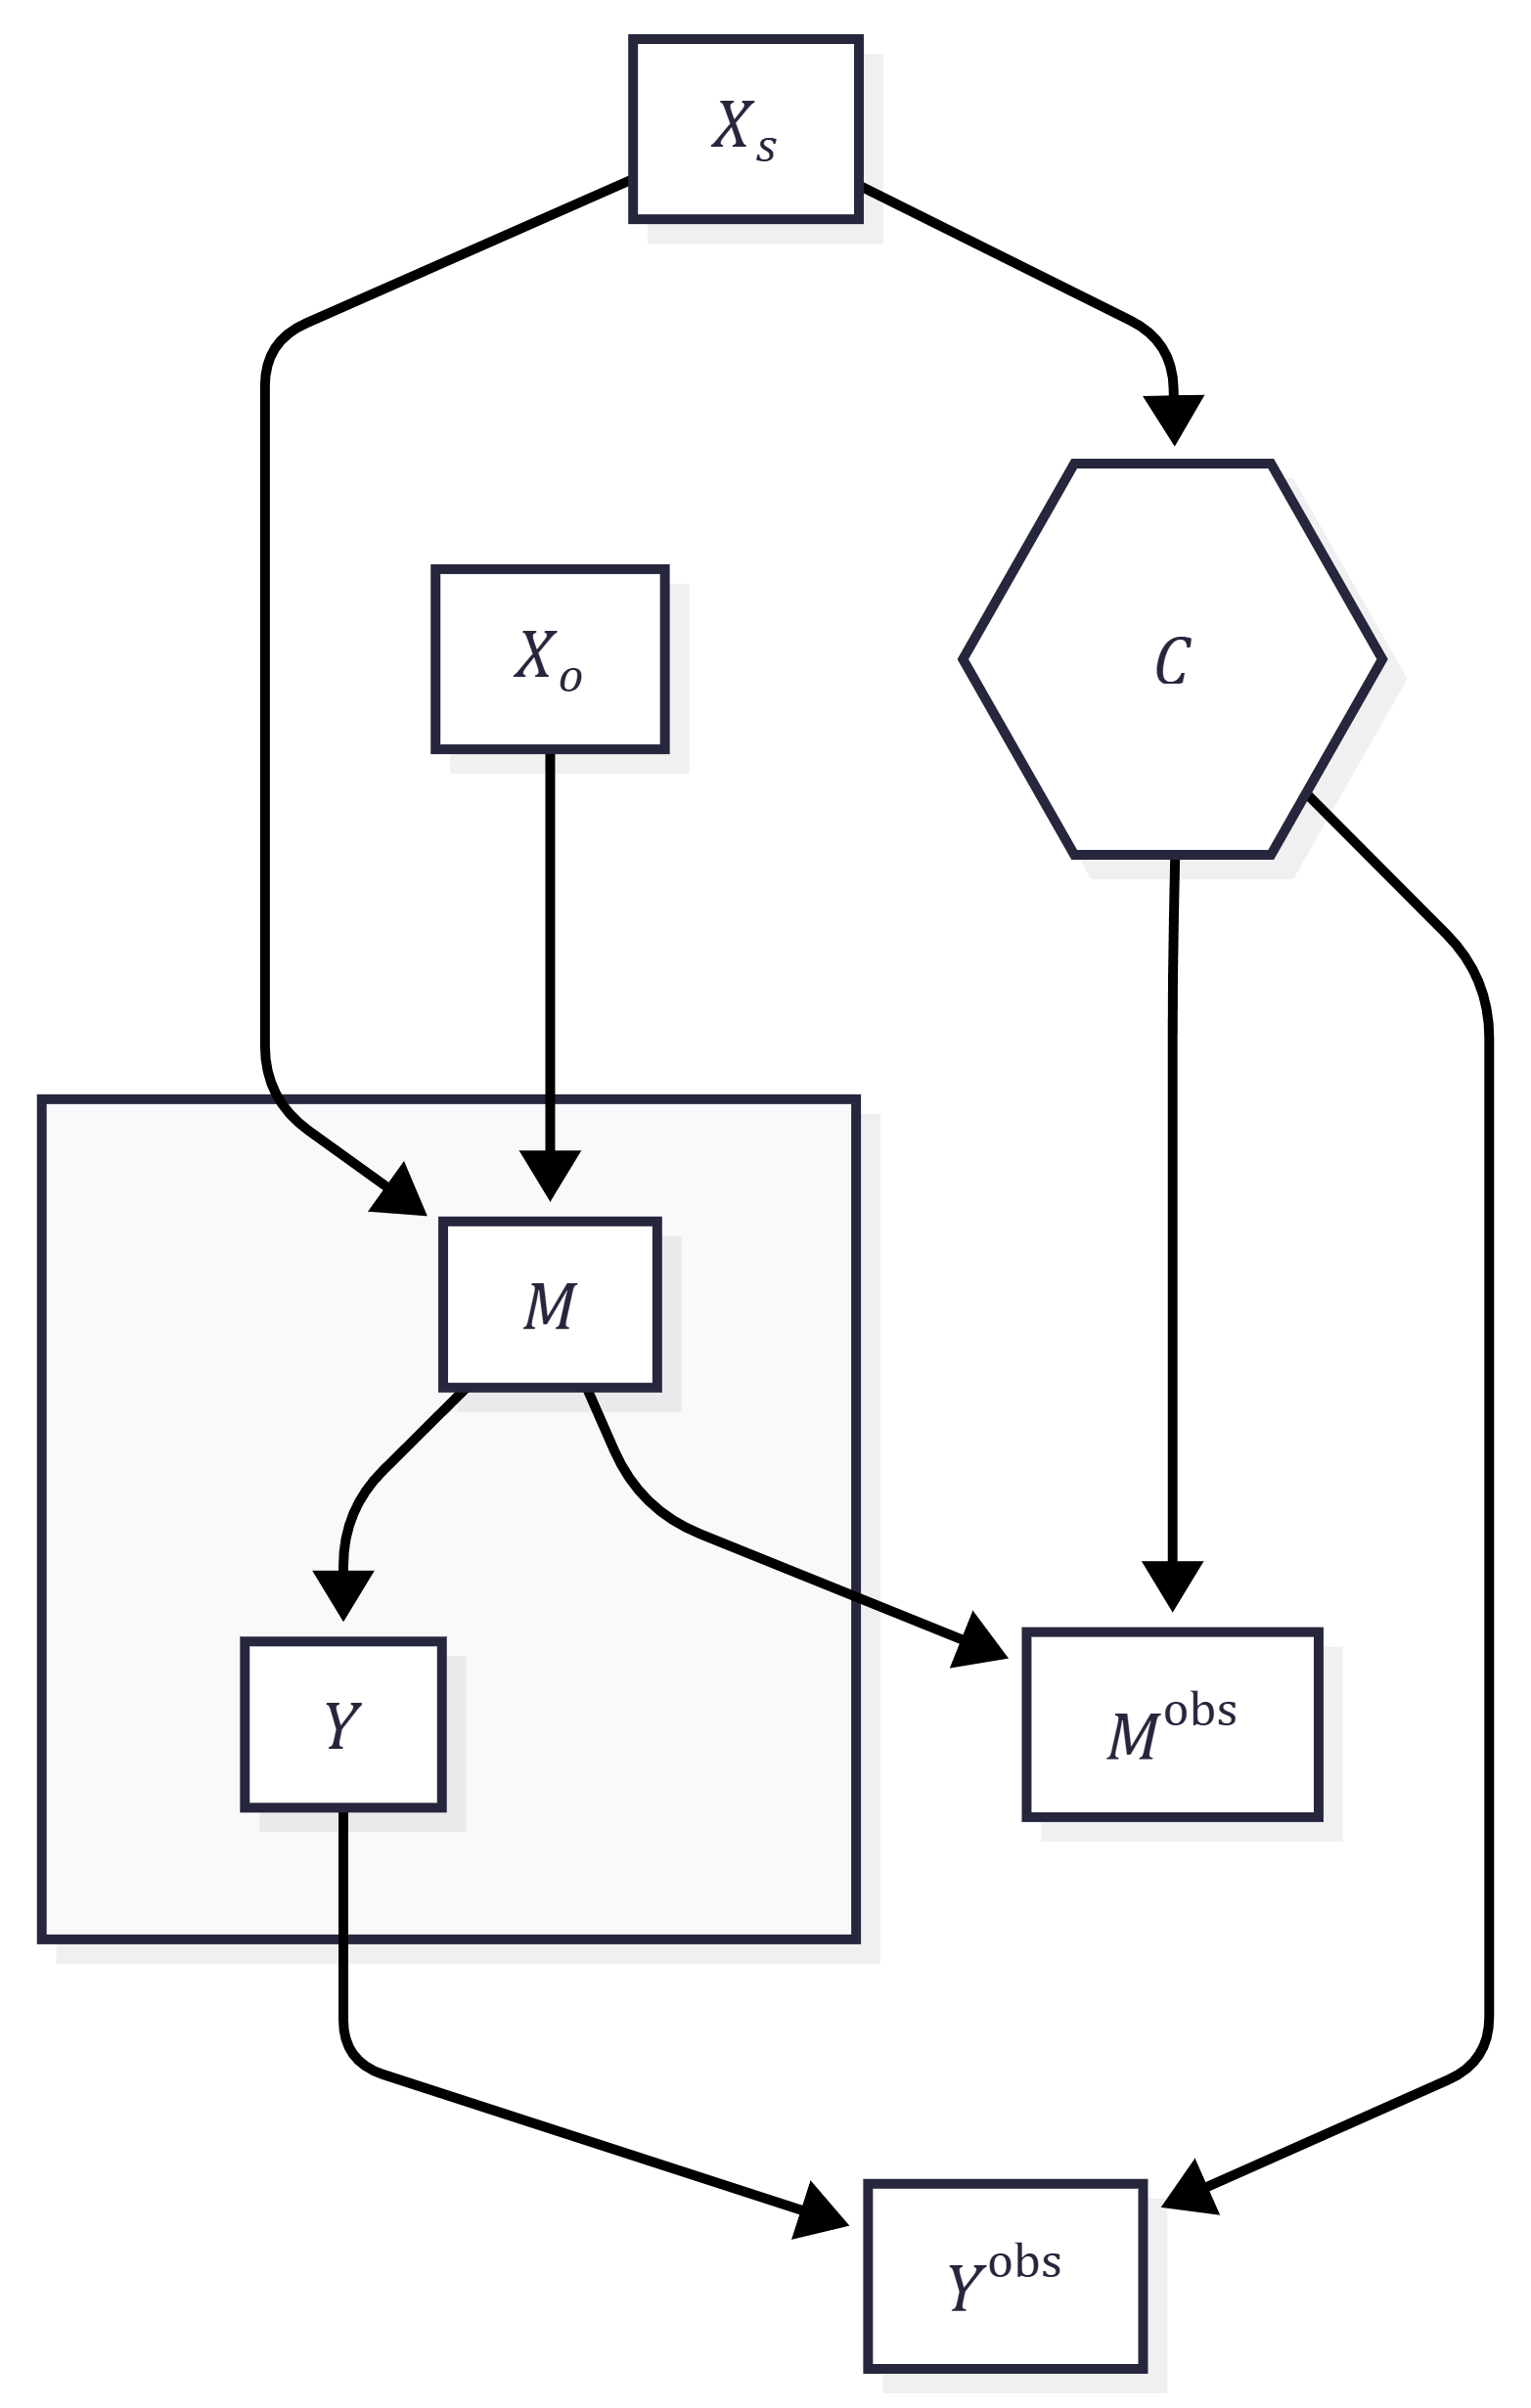
\includegraphics[width=0.425\linewidth]{figures/figure2_1.png}
\caption*{Figure 2.1. The causal DAG induced by the SCM in Definition 2.1 (exogenous $U$ nodes omitted). Four levels read top to bottom. Level 1: $\mathbf{X}_s$ and $X_o$, the upstream features, always observed for all units. Level 2: $C$, the compliance gate, with $\mathbf{X}_s$ as its sole parent; $X_o$ has no path to $C$. Level 3: $M$ and $Y$, the latent mediators and outcome; $M$ has parents $\mathbf{X}_s$ and $X_o$; $Y$ has $M$ as its sole parent; both exist for all units. Level 4: $M^{\text{obs}}$ and $Y^{\text{obs}}$, the analyst-observed quantities; each has two parents: the corresponding latent variable and $C$.}
\end{figure}

\textbf{Condition 1: Unit-level threshold selection.}

The compliance decision is made independently for each unit $i$ based solely on whether $\mathbf{X}_{s,i}$ falls within $\mathcal{R}$:

\[
C_i \leftarrow \mathbf{1}\{ \mathbf{X}_{s,i} \in \mathcal{R} \}.
\]

There is no discretion, no group-level assignment, and no partial compliance. Consequently, $Y_i^{\text{obs}}$ is non-missing if and only if $C_i = 1$.

Threshold-based programmes are the most common regulatory design. In such programmes, each selection variable $X_{s,j}$ is compared against a fixed threshold $T_j$, and the compliance region takes the form

\[
\mathcal{R} = \{ \mathbf{x} \in \mathbb{R}^k : x_j \geq T_j \text{ for all } j = 1, \ldots, k \},
\]

an intersection of half-spaces. Programmes that trigger compliance on any one criterion (OR logic) define $\mathcal{R}$ as a union of half-spaces instead. The formulation $\mathbf{X}_{s,i} \in \mathcal{R}$ accommodates both without modification.

This threshold-assignment rule is the same structure studied in regression discontinuity designs, where treatment switches as a running variable crosses a cutoff (\cit{leelemieux2010}{Lee \& Lemieux, 2010}). The two settings differ in aim: regression discontinuity uses the cutoff to identify a treatment effect among units near it, whereas Condition 1 uses it to determine which units are observed at all. Condition 1 also assumes that units do not manipulate $\mathbf{X}_s$ to select a side of the threshold. This assumption can fail when reporting is costly: the bunching literature documents units adjusting a choice variable to sit just below regulatory kinks and notches (\cit{kleven2016}{Kleven, 2016}). It is most secure when the selection variable is hard to manipulate, as with the gross floor area that gates the Chicago benchmarking obligation of Section 4.

\textbf{Condition 2: Endogenous selection variable.}

$\mathbf{X}_s$ appears as a causal argument in $f_M$ with non-zero effect: for at least one $j \in \{1, \ldots, k\}$, $f_M$ is non-constant in $X_{s,j}$, meaning there exist two values of $X_{s,j}$ that, with all other arguments of $f_M$ held fixed, yield different values of $M$. When $X_{s,j}$ is continuous and $f_M$ is differentiable, this is the familiar condition

\[
\frac{\partial f_M}{\partial X_{s,j}} \neq 0.
\]

The non-constancy form is the one the definition requires, since selection variables may be categorical, as with the property classes that co-determine the Chicago gate (Section 4), where a derivative is undefined.

Combined with $M \in \mathrm{pa}(Y)$ (the set of direct causal parents of $Y$ in the DAG) in the structural equation for $Y$, this guarantees at least one directed path $X_{s,j} \rightarrow M \rightarrow Y$ in the DAG induced by $\mathcal{F}$. The selection variables are not merely correlated with $Y$ through a common cause; they are causes of $Y$'s causal parents.

\textbf{Condition 3: Atomic reporting requirement.}

A unit reports all outcome data or none. For each unit $i$:

\[
M_i^{\text{obs}} = \begin{cases} M_i & \text{if } C_i = 1 \\ \emptyset & \text{if } C_i = 0 \end{cases}, \qquad Y_i^{\text{obs}} = \begin{cases} Y_i & \text{if } C_i = 1 \\ \emptyset & \text{if } C_i = 0 \end{cases}
\]

This restates what the SCM equations already encode: since $M^{\text{obs}}$ and $Y^{\text{obs}}$ are both gated by the same scalar $C$, partial reporting is structurally impossible.

The SCM implies that the analyst observes $\mathbf{X}_{s,i}$, $X_{o,i}$, and $C_i$ for every unit $i$, and additionally $M_i^{\text{obs}} = M_i$ and $Y_i^{\text{obs}} = Y_i$ for units with $C_i = 1$. Figure 2.1 above shows the causal DAG induced by Definition 2.1.

\textbf{Remark on necessity.}

Condition 1 alone produces a selected sample with MAR missingness, because $C$ is a deterministic function of observed $\mathbf{X}_s$. Yet it is not necessarily biased with respect to the $X$--$Y$ relationship. It is Condition 2 that makes the truncation analytically consequential: because $\mathbf{X}_s$ causes both selection and outcome, the compliant subsample is systematically enriched on $Y$ relative to the full population. Condition 3 distinguishes compliance-gated data from item non-response, where individual fields may be selectively missing. Their joint satisfaction produces the selection bias characterised in Section 2.2 and the documentation structure that makes DAG falsification tractable (Section 2.3).

Note that $f_M$ and $f_Y$ are left unspecified at the class level: the class definition constrains the causal graph structure and rules out degenerate $f_M$ (Condition 2), but leaves the specific functional forms of $f_M$ and $f_Y$ otherwise unspecified. Identifying the functional forms from institutional documentation is precisely the task of Stage 3 of the TDGP pipeline (Section 3.3). The scalar $Y$ likewise denotes a single factor of interest, the quantity a given study sets out to explain; a dataset may admit several such factors, each of the form $Y_k = f_{Y_k}(M)$, and the analyst instantiates the outcome role with whichever the research question selects (Section 3.2).

\textbf{Remark on the constitutive assumption.} The structural equations above are taken to be the rules the programme publishes, read from its governing documents (Section 2.3). The pipeline therefore rests on one premise: that the institution generates the data by the rules it sets down, so that those documents specify this structure with authority rather than merely describe it. The disturbance terms carry whatever the rules do not; a procedure applied with perfect uniformity would make $f_M$ and $f_Y$ deterministic, and the $U$ terms are the degree to which realized application departs from the documented rule. What the documents cannot supply is exogeneity: that these disturbances are mutually independent and uncorrelated with the features, the Markovian premise any structural model makes (\cit{pearl2009}{Pearl, 2009}), is assumed here as in any causal study, not read from a document. The constitutive premise occupies the place the asserted graph holds in an ordinary study, but on a firmer footing, an external authority rather than the analyst's judgement. Its further advantage is that it fails auditably: where the documented form leaves an empirical signal, a departure surfaces as a failed reconstruction or a gate discrepancy (Section 3.3) rather than in silence.

\subsection{The Selection Bias This Class Induces}

The analyst observes the set $\mathcal{O} = \{\mathbf{X}_s, X_o, C, M^{\text{obs}}, Y^{\text{obs}}\}$ and wants to study the outcome $Y$, to explain its variation and to predict it. The set is read unevenly: the upstream features and the compliance indicator are seen for every unit, but the outcome and the mediators only when $C = 1$, since $Y^{\text{obs}}$ and $M^{\text{obs}}$ are empty for all units with $C_i = 0$. The dataset is therefore not a sample drawn from a larger population; it may well cover the entire population, with the compliance gate acting as a missingness mechanism, not a sampling one.

Faced with this structure, an analyst has two paths. The first is to proceed with complete-case analysis: drop the units where $Y^{\text{obs}}$ is null and treat the remaining rows as sufficient for the analysis. This is the default behaviour of most statistical and machine-learning workflows, which silently discard incomplete rows. The second path is to treat the missingness as informative: to recognise that $Y^{\text{obs}} \neq Y$, that the units with absent outcomes are not random absences, and to actively correct for the difference. Proposition 2.1 below establishes formally how the first path fails. 

\textbf{Proposition 2.1 (Compliance-Gate Selection Bias).} Under Definition 2.1, suppose

(i) $P(\mathbf{X}_s \in \mathcal{R}) \in (0,1)$: the population contains both compliant and non-compliant units; and

(ii) $E[Y \mid C = 1] \neq E[Y \mid C = 0]$: the two compliance groups differ in expected outcome.

Then the expected outcome among compliant units differs from the population expected outcome:

\[
E[Y \mid C = 1] \neq E[Y].
\]

\textit{Proof.} The compliance criterion partitions the population into compliant units ($\mathbf{X}_s \in \mathcal{R}$) and non-compliant units ($\mathbf{X}_s \notin \mathcal{R}$). By the law of total expectation,

\[
E[Y] = E[Y \mid C = 1]\, P(C = 1) + E[Y \mid C = 0]\, P(C = 0).
\]

Suppose for contradiction that $E[Y \mid C = 1] = E[Y]$. Substituting and rearranging gives $E[Y \mid C = 1]\, P(C = 0) = E[Y \mid C = 0]\, P(C = 0)$, and since $P(C = 0) > 0$ by (i), this forces $E[Y \mid C = 1] = E[Y \mid C = 0]$, contradicting (ii). The compliance gate sets $Y^{\text{obs}} = \emptyset$ for all units with $\mathbf{X}_s \notin \mathcal{R}$, so complete-case analysis retains only the compliant group and computes $E[Y \mid C = 1]$, which is not $E[Y]$. $\square$

\textbf{Remark on condition (ii).} Condition (ii) is where Condition 2 of Definition 2.1 does its work, and the proposition states it as a hypothesis rather than deriving it, because the derivation does not go through as pure logic. Condition 2 guarantees that $f_M$ is non-constant in at least one component of $\mathbf{X}_s$, so the two groups pass systematically different inputs through the same structural functions: compliant units draw $\mathbf{X}_s$ from within $\mathcal{R}$, non-compliant units from outside it. What Condition 2 does not rule out is exact cancellation, since a non-constant function can still average to the same value over two disjoint regions. Equality of the two group means would require the variation of $f_M$ across the threshold to cancel exactly against the distribution of $\mathbf{X}_s$, a knife-edge that nothing in the institutional design protects and that any perturbation of the input distribution would break. Condition (ii) is therefore the generic case for the class. For the threshold programmes that motivate it, the case is stronger still: a programme gates on a measure of scale precisely because scale drives the outcome it exists to measure, so units above the threshold are enriched on $Y$ by the programme's own design logic. Section 4 exhibits the difference directly in the Chicago data, where compliant buildings are systematically larger and emissions scale near-proportionally with size.

The error arises at the inferential step. $Y^{\text{obs}}$ is not wrong: for every compliant unit, $Y_i^{\text{obs}} = Y_i$ exactly, and the complete cases are internally consistent. The error is not in the data but in what the analyst does with it: using statistics computed from $Y^{\text{obs}}$ as if they described the full population, when in fact they describe only the subset of units whose outcomes were made observable by the compliance gate.

From the analyst's perspective, the error is invisible at the analysis stage. The complete cases look like a coherent dataset: the rows are fully populated, the model converges, the metrics are reasonable. Nothing in the output signals that non-compliant units exist or that their outcomes were systematically different from those of compliant units. The bias is structural, a property of the institutional rule that generated the data rather than of the analysis itself, and it persists regardless of sample size. Even if the analyst had records for every unit in the population, the compliance gate would still withhold $Y$ for every non-compliant unit, leaving the bias exactly as severe. A better or larger sample is not the answer; the missing values are not absent by chance, and no amount of data can supply what the compliance gate withholds.

The cause of missingness determines the correction. Knowing that the bias exists is not sufficient to correct it. The form of the correction depends on what drives the missingness, specifically on whether the probability of a unit's outcome being absent depends on the outcome itself or only on other observed variables. Different answers lead to different corrections, and some missingness patterns are not correctable at all from observed data alone.

To classify the mechanism, introduce $R_i = 1 - C_i$ as the missingness indicator for unit $i$: $R_i = 1$ when $Y_i^{\text{obs}}$ is absent, $R_i = 0$ when observed. \cit{rubin1976}{Rubin (1976)} distinguishes three categories based on what $P(R_i = 1 \mid Y_i, \mathbf{X}_{s,i}, X_{o,i})$ depends on. Under \textbf{MCAR} (Missing Completely At Random), the probability of missingness is unrelated to any characteristic of the unit; absences are literally random. Under \textbf{MAR} (Missing At Random), missingness depends only on observed variables: once those are conditioned on, the absent value carries no additional information about why it is missing. Under \textbf{MNAR} (Missing Not At Random), the probability of missingness depends on the unobserved value $Y_i$ itself: for example, firms with worse financial outcomes selectively withhold voluntary disclosure, making the absent values informative in a way that cannot be recovered from observed data alone.

Compliance-gate data is MAR. From the SCM, the compliance decision is made by comparing $\mathbf{X}_{s,i}$ against $\mathcal{R}$. Nothing about $Y_i$ enters that decision. The probability that unit $i$'s outcome is absent is:

\[
P(R_i = 1 \mid Y_i,\, \mathbf{X}_{s,i},\, X_{o,i}) = \mathbf{1}\{\mathbf{X}_{s,i} \notin \mathcal{R}\}.
\]

In this expression, the left-hand side is the probability of missingness given full knowledge of the unit, including its latent $Y_i$. The right-hand side is the indicator that $\mathbf{X}_{s,i}$ falls outside $\mathcal{R}$, a function only of the always-observed $\mathbf{X}_{s,i}$. The value of $Y_i$ on the left plays no role. Once $\mathbf{X}_{s,i}$ is known, the compliance decision is deterministic: the conditional probability is 0 or 1, not a number between them. This is MAR: the missingness is fully explained by an observed variable, and the missing outcome values carry no additional information about why they are absent.

The MAR classification is consequential. Because the missingness mechanism is fully characterised by $\mathbf{X}_s$, it can be modelled using the data already in hand. Estimating the probability that a unit was required to report, $P(C = 1 \mid \mathbf{X}_s, X_o)$, and reweighting the complete cases by its inverse corrects the bias across the region the gate leaves populated. Treated this way, the missingness indicator $R$ is itself a node in the causal graph, placing the analysis within the missingness-graph framework of \cit{mohanpearl2021}{Mohan and Pearl (2021)}, whose graphical criteria identify when a target distribution is recoverable from incomplete data. The reweighting reaches only as far as that overlap: where the threshold leaves no compliant units to carry the weight, the target is not recoverable by reweighting alone, and recovery there passes to the structural form (Section 3.4). A further assumption underwrites the correction even within the overlap: the deterministic gate makes selection ignorable given $\mathbf{X}_s$ by construction, but where realized compliance departs from the documented rule, that ignorability becomes an assumption on the observed features rather than a consequence of the gate (Sections 3.1, 3.4). This is the logic of inverse probability weighting, which Section 5 implements.

The MAR structure also locates this class relative to the econometric sample-selection tradition. \cit{heckman1979}{Heckman (1979)} treats selection bias as a specification error and corrects it with a two-step estimator; that machinery is built for samples whose selection may depend on unobservables correlated with the outcome equation, the MNAR configuration, and in its classical form it buys identification with distributional assumptions on the joint error structure or an exclusion restriction. The compliance gate needs none of that apparatus: selection is a documented, deterministic function of observed covariates, so the missingness is MAR and inverse probability weighting on an estimated propensity identifies the recoverable region without distributional assumptions on the outcome equation. That economy is a direct payoff of the class structure rather than a methodological preference. The two approaches remain complements: where realized compliance departs from the documented rule in ways that track unobservables, the configuration drifts toward the one Heckman's estimator was built for, and the selection-ignorability assumption of Section 3.4 is what bounds that drift.

Cross-validation does not detect this bias. In a standard $k$-fold cross-validation, both training and test folds are drawn from the complete cases, the units where $Y^{\text{obs}}$ is non-null. The test fold is subject to the same compliance gate as the training fold: it contains only units with $\mathbf{X}_s \in \mathcal{R}$, not a draw from the full population. What cross-validation measures is how well the model captures $E[Y \mid \mathbf{X}_s, X_o, C = 1]$, the conditional expectation within the compliant subsample. A model can achieve excellent performance on this criterion while still producing biased estimates of the population-level $E[Y \mid \mathbf{X}_s, X_o]$. Cross-validation tests model fit on the complete cases; it does not test whether the complete cases are representative of the population.

\subsection{Why DAG Falsification Is Tractable for This Class}

The central obstacle to applied causal inference is not estimation but specification. Once a directed acyclic graph (DAG) is fixed, Pearl's framework converts identification questions into estimation procedures: the do-calculus rewrites interventional quantities such as $P(Y \mid do(X))$ in terms of observational quantities whenever the DAG permits; the back-door and front-door criteria pick out which variables to adjust for in order to block confounding paths or to exploit a fully observed mediating chain; counterfactual identification extends the same machinery to queries about what would have happened under alternative interventions. Every step in this pipeline rests on a single explicit assumption: that the DAG faithfully represents the data-generating process. Once that assumption is granted, the rest follows mechanically. The difficulty lies upstream, at the point where the DAG itself is proposed. In most observational studies, the DAG is asserted on the basis of subject-matter expertise: the analyst draws arrows between variables, defends the choices in prose, and proceeds. The arrows are not derived from an authoritative external source, and observational data alone is generally insufficient to distinguish between DAGs that imply incompatible causal estimands (\cit{pearl2009}{Pearl, 2009, Ch. 2}). This is the DAG falsification problem.

Compliance-gated datasets are unusual in this regard. The documentation is constitutive, not descriptive: legislation, regulatory rules, and technical reporting standards are the \textit{primary source} of the compliance obligation, not a secondary description of it. A building falls under a benchmarking ordinance because the ordinance text says it does; a firm files a financial disclosure because the SEC rules say it must. The institutional documents are in force before any data is collected, and they specify in operational detail what must be reported, by whom, and how the reported quantities are calculated. This documentation is not commentary on the data-generating process; it is the written specification of the institutional rules that produce the dataset.

Three components of the DAG induced by Definition 2.1 map directly onto three components of this documentation. The selection rule, which determines which units must report and on what criterion, is specified by the threshold provision of the regulation; this is exactly Condition 1 of Definition 2.1, and it identifies $\mathbf{X}_s$, $\mathcal{R}$, and the structural equation for $C$. The reporting schema, which determines which variables must be filed by compliant units, is specified by the regulation's enumeration of required fields; this identifies $M^{\text{obs}}$ and $Y^{\text{obs}}$, and through them the latent $M$ and $Y$. The functional structure linking reported variables to the outcome, typically given as an accounting formula, emissions factor, or measurement standard, is specified by the technical annex of the regulation; this identifies $f_Y$ and the parent set $\mathrm{pa}(Y)$. These three mappings cover exactly what Definition 2.1 leaves to be supplied per application: the identities of $\mathbf{X}_s$, $M$, and $Y$; the compliance region $\mathcal{R}$; and the functional form $f_Y$. The class definition and the documentation are complementary by construction: the SCM provides the skeleton, the documentation provides the flesh.

One structural feature lies outside this correspondence: the upstream-to-mediator edges $\mathbf{X}_s \to M$ and $X_o \to M$, by which the upstream features produce the mediators. The mediators are measured, not computed from a rule, so no document constitutes these links; they are confirmed the ordinary way, by checking that the upstream features predict $M$ in the data. That they rest on association rather than the constitutive source is harmless, because they bear on whether the bias exists, not on whether the correction is valid. For the bias to exist the analysis needs only that $\mathbf{X}_s$ be among the causes of $M$ (Condition 2), which the data settle directly; the validity of the correction rests instead on the documented gate, on $\mathrm{pa}(Y) = M$, and on selection being ignorable given the observed features (Section 3.4), and the analysis conditions on $X_o$ whether or not $X_o \to M$ holds.

The consequence is that the DAG becomes testable, not merely assertable. Because the documentation supplies the very components the graph hypothesises, each conjecture can be set against the provision that fixes it: a conjectured selection variable against the threshold provision, a conjectured mediator or outcome against the reporting schema, the parent set of $Y$ against the technical formula. A conjecture the documentation contradicts is refuted, and the provision that contradicts it names the correction, so the candidate graph can be brought into line with the source rather than merely defended. This is a test against an authoritative external standard, and it reaches a conclusion that argument from domain expertise alone cannot. One of the three components leaves an empirical mark as well: because the formula computes $Y$ from $M$, the documented mediators should reconstruct the reported outcome within the compliant subset, so the data can corroborate $\mathrm{pa}(Y) = M$ on that one link. These three components, though, are settled by the documents whether or not that mark is read.

In a general observational dataset, no equivalent primary source exists. The substitutes available to the analyst are codebooks, expert opinion, and prior literature, and each falls short. A codebook documents fields, not causal relationships. Subject-matter experts can be consulted, but expert opinion is contestable and does not produce a falsifiable functional form. Prior literature can be invoked, but it inherits the same problem one step removed: the DAGs proposed in earlier studies were themselves typically asserted by their authors rather than tested against an external source, and grounding a new DAG on them only chains one assertion to another without anchoring the structure in anything that could refute the chain.

This tractability is what justifies treating compliance-gated datasets as a distinct analytical class. The DAG must still be subjected to a falsification test, since that work does not happen automatically, but the ingredients required to carry it out are present in the documentation. Section 3 operationalises this insight; Section 4 carries it out on the Chicago Energy Benchmarking dataset.

\subsection{Scope of the Class}

This section shows that real reporting programmes belong to the class. Mandatory-reporting regimes across energy, labour, environmental, and financial regulation all satisfy the three conditions of Definition 2.1. The Chicago benchmarking data of Section 4 is therefore one instance of the class rather than the whole of it.

The common pattern is a size threshold. Regulators rarely impose reporting obligations uniformly. They exempt small units to limit administrative burden and target the units whose activity dominates the outcome the programme exists to measure. The exemption is written as a threshold on an observable measure of scale, and that same measure of scale is a cause of the outcome. This is precisely the configuration of Conditions 1 and 2: the selection variable is a threshold-gated measure of size (Condition 1), and size drives the reported outcome through the programme's mediators (Condition 2). Table 2.2 maps four programmes onto the class.

\par\medskip\noindent
{\small\itshape \textbf{Table 2.2. Four compliance-gated reporting programmes mapped onto Definition 2.1.} Each programme gates a reported outcome on a size threshold, and the selection variable is a cause of that outcome. The final column names the constitutive document that, per Section 2.3, encodes the selection rule, the reporting schema, and the outcome's functional form.\par}
\nopagebreak\medskip\nopagebreak
{
\footnotesize
\setlength{\tabcolsep}{5pt}
\renewcommand{\arraystretch}{1.15}
\begin{longtable}{>{\raggedright\arraybackslash}p{\dimexpr 0.146\linewidth-2\tabcolsep\relax}>{\raggedright\arraybackslash}p{\dimexpr 0.146\linewidth-2\tabcolsep\relax}>{\raggedright\arraybackslash}p{\dimexpr 0.356\linewidth-2\tabcolsep\relax}>{\raggedright\arraybackslash}p{\dimexpr 0.2\linewidth-2\tabcolsep\relax}>{\raggedright\arraybackslash}p{\dimexpr 0.152\linewidth-2\tabcolsep\relax}}
\toprule
Programme & Selection variable $\mathbf{X}_s$ & Compliance region $\mathcal{R}$ & Reported outcome $Y$ (via mediators $M$) & Constitutive document \\
\midrule
\endfirsthead
\toprule
Programme & Selection variable $\mathbf{X}_s$ & Compliance region $\mathcal{R}$ & Reported outcome $Y$ (via mediators $M$) & Constitutive document \\
\midrule
\endhead
\bottomrule
\endlastfoot
Municipal energy benchmarking & Gross floor area & Area $\geq$ threshold (50,000 sq ft in Chicago) & GHG emissions, via metered fuel use & Benchmarking ordinance; EPA emission-factor tables \\
OSHA injury recordkeeping & Establishment employee count & More than 10 employees, outside exempt industries & Recordable injury and illness counts, via worker-hours of exposure & 29 CFR Part 1904 \\
EPA Toxics Release Inventory & Employee count \textit{and} chemical throughput & $\geq$ 10 FTE-equivalents AND > 25,000 lb manufactured/processed (or > 10,000 lb otherwise used) of a listed chemical & Annual chemical releases, via production volume & EPCRA §313; 40 CFR Part 372 \\
SEC accelerated-filer disclosure (boundary case) & Public float & Public float $\geq$ \$75 million & Enhanced financial disclosures, via firm scale of operations & Exchange Act Rule 12b-2 (17 CFR §240.12b-2) \\
\end{longtable}
}
\par\medskip

\textit{Boundary case:} SEC disclosure satisfies Conditions 1 and 2, but Condition 3 only for individual gated items, not the filing as a whole (see below).

Municipal energy benchmarking, the first row of the table, is the member that Section 4 develops in full using the Chicago Energy Benchmarking data. This section works through the other three. Taken in turn, OSHA recordkeeping, the EPA Toxics Release Inventory, and SEC disclosure show both the range of the class and where its conditions bind.

\textbf{OSHA injury recordkeeping.} An establishment with ten or fewer employees at all times in the prior calendar year is partially exempt from injury and illness recordkeeping (\cit{osha2001}{OSHA, 2001, §1904.1}), as are establishments in designated low-hazard industries (§1904.2). Employee count is the selection variable, and the threshold defines $\mathcal{R}$ (Condition 1). It also causes the outcome: more employees mean more worker-hours of exposure, and recordable injuries accumulate with exposure, so selection acts on the outcome through an operational-scale mediator (Condition 2). A unit keeps the full log or none, the atomic requirement of Condition 3. Complete-case analysis over the recorded establishments would describe injury rates among larger firms, not the full population of workplaces.

\textbf{EPA Toxics Release Inventory.} The TRI is the cleanest illustration of the AND-logic compliance region of Condition 1. A facility must file an annual release report only if it meets three criteria at once (U.S. EPA, 40 CFR §372.22): it operates in a covered industry sector, employs the equivalent of ten or more full-time staff, and manufactures or processes more than 25,000 pounds, or otherwise uses more than 10,000 pounds, of a listed chemical (40 CFR §372.25). The region $\mathcal{R}$ is thus an intersection of half-spaces. Chemical throughput, one component of $\mathbf{X}_s$, directly causes releases: a facility that processes more of a chemical has more to release. Condition 2 holds through this path, and releases are gated atomically with the rest of the Form R, satisfying Condition 3.

\textbf{SEC disclosure thresholds.} SEC disclosure partially qualifies, and marks the boundary of the class. Conditions 1 and 2 hold: Exchange Act Rule 12b-2 (SEC, 17 CFR §240.12b-2) classifies an issuer as an accelerated filer once its public float reaches \$75 million, and public float scales with the operations that generate the disclosed financials. Condition 3 does not hold for the filing as a whole, because every public issuer files a Form 10-K regardless of size; the threshold toggles the stringency of disclosure, not its existence. Membership holds only at the level of an individual gated item, such as the auditor's attestation on internal control over financial reporting, which appears above the threshold and is absent below it.

All four examples supply what the falsification test of Section 2.3 needs: a constitutive document in force before any data was collected. The benchmarking ordinance points to the EPA emission-factor tables; the TRI rules incorporate published release-estimation methods; OSHA's regulation defines what counts as a recordable case. Wherever such a document exists, the DAG can be tested rather than merely asserted.

These programmes are illustrative, not a complete inventory. The criterion they share is general: a written rule that predates the data, fixes which units are recorded, and turns on a cause of the outcome. Nothing about that criterion is peculiar to government regulation. Many private-sector datasets are generated the same way. Consider a lender's loan book. The selection variable $\mathbf{X}_s$ is the applicant's credit score; the compliance region $\mathcal{R}$ is the set of scores at or above the approval cutoff written into the lender's credit policy; and the reported outcome $Y$ is repayment behaviour, recorded only for the applicants the cutoff admits. The credit policy is fixed before any loan is issued, and the score that triggers approval is itself a cause of repayment, so Conditions 1 and 2 hold exactly as in the regulatory cases. The same structure recurs wherever a written rule decides what is recorded: an insurer underwriting from an eligibility manual, a clinical registry enrolling only patients who meet pre-specified inclusion criteria, a marketplace logging only the transactions its published rules permit. Each is governed by a process fixed before the data exists, and each gates observation on a variable that also drives the outcome.

What defines membership, then, is not the domain, nor whether the governing rule is public law or internal policy, but whether the analyst can obtain the document that states it. When that document is available, as it is for the regulatory programmes above, the data-generating process is recoverable and the falsification test of Section 2.3 can be run. When it is proprietary and withheld, the process is still constitutive but no longer recoverable, and the dataset falls back to the ordinary observational case in which the DAG can only be asserted. The class is broad on this criterion, and the pipeline of Section 3 applies to any member whose governing document can be read; the Chicago Energy Benchmarking data is simply where this paper carries the procedure out in full.


\FloatBarrier
\section{The Tested Data-Generating Process Pipeline}

A dataset is not a transcript of the world; it is the record an institution chose to keep. Standard workflows read the rows at face value and so assume the recording process is innocuous, that what was written down is a fair sample of what happened. For compliance-gated data that assumption fails: the institution layer of the structural model (Section 2.1) decides what is observed, and it does so on a variable that also drives the outcome (Section 2.2). Before modelling how the world produces outcomes, the analyst must therefore characterise how the institution decided what to record. The most direct evidence about that recording layer is the pattern of what is absent.

The TDGP pipeline operationalises this discipline. From any dataset satisfying Definition 2.1 it returns a DAG that has survived a falsification test, in three stages: read the recording layer from the data (Stage 1); hypothesise the world layer that generated the recorded values (Stage 2); and test that hypothesis against the primary documentation that defines the institution (Stage 3). The same discipline governs the analysis that the tested DAG later licenses in Sections 4 onward: the observed data is always treated as a filtered view, never as the population itself. The pipeline is dataset-agnostic; Section 4 carries it out on the Chicago Energy Benchmarking data.


\subsection{Stage 1: Shadow Matrix Analysis}

The analyst does not arrive at the data empty-handed. The documentation already supplies a hypothesis: that the dataset is compliance-gated, with reporting switched by some selection rule. What the documentation cannot supply is whether that hypothesis holds in the data at hand, and how the abstract gate maps onto the specific columns of the file. Stage 1 settles both, and it does so from the data alone, so that the recording structure is established independently of the documentary claims it will be tested against in Stage 3.

What does a gate look like in the data? A single institutional switch leaves a particular trace. Its mark is not that individual fields are missing but that they are missing together: every field the gate governs is observed for the same units and absent for the same units, because one decision controls them all. Detecting the gate is therefore a question of co-missingness: which variables vanish in concert. The natural summary of co-missingness across a dataset is the correlation between columns' missingness indicators, so that correlation, not the raw rate of missingness, is the quantity Stage 1 computes.

Concretely, for each unit $i$ and variable $j$, define the missingness indicator $R_{ij} = \mathbf{1}\{X_{ij} \text{ is missing}\}$, equal to 1 where the value is absent and 0 where it is observed. The shadow matrix is the $p \times p$ matrix of pairwise correlations among the indicator columns $R_1, \ldots, R_p$: its $(j, k)$ entry is the correlation between the missingness of variables $j$ and $k$ (the phi coefficient, for binary indicators), large when the two fields tend to be absent on the same units. Reading this matrix for structure is the whole of Stage 1.

The compliance-gate hypothesis makes sharp predictions about these correlations, and three regimes are distinguishable.

\textbf{Idiosyncratic missingness.} Off-diagonal correlations near zero mean variables go absent independently of one another. This is the signature of data missing completely at random (MCAR), under which complete-case analysis and standard imputation are unbiased (\cit{littlerubin2002}{Little \& Rubin, 2002}). A compliance-gated dataset does not look like this; observing it would refute the hypothesis.

\textbf{Block structure.} A set of variables that goes missing in lockstep, each absent almost exactly when the others are, is the empirical fingerprint of an atomic reporting gate (Condition 3 of Definition 2.1): a single switch that withholds the whole block at once. The structural model predicts this directly: because $M^{\text{obs}} = C \cdot M$ and $Y^{\text{obs}} = C \cdot Y$ are gated by the same $C$, every one of their missingness indicators reduces to $1 - C$, so the gated fields should share a single missingness pattern and correlate almost perfectly.

\textbf{Gate alignment.} Block structure shows a co-missing block; the observed $C$ shows that the compliance gate is what produces it. In the DAG, $C$ is a direct cause of the missingness ($C \to M^{\text{obs}}$, $C \to Y^{\text{obs}}$): by the institution equations $M^{\text{obs}} = C \cdot M$ and $Y^{\text{obs}} = C \cdot Y$, a field is withheld precisely when $C = 0$. The check is to correlate the observed values of $C$ against each field's missingness indicator $R_j$. Note what is being correlated: the value of $C$ against $R_j$, not the missingness of $C$ against the other indicators, since $C$ is observed for every unit and is never itself absent. For the gated fields the relationship is exact, $R_{ij} = 1 - C_i$, a correlation of $-1$; the fields whose missingness $C$ explains this way are the gated outcome and mediator set $\{M^{\text{obs}}, Y^{\text{obs}}\}$. ($C$ is observed throughout, which is also what makes the later IPW correction possible.)

Identifying the gated block does not exhaust the shadow matrix: the blanks in a real file come from several mechanisms, told apart by how they relate to $C$.

\begin{itemize}
  \item \textbf{Gate-missingness.} A field absent exactly when $C = 0$ ($R_{ij} = 1 - C_i$). This is the MAR mechanism the pipeline corrects.
  \item \textbf{Selection-side discrepancy.} Compliance does not follow the threshold cleanly: eligible units fail to report, exempt units report anyway, enforcement is uneven. Whether the observed $C$ departs from the documented rule $\mathbf{1}\{\mathbf{X}_s \in \mathcal{R}\}$ is a question for Stage 3, once that rule is in hand.
  \item \textbf{Reporting-side discrepancy.} A gated unit files partially or with error: partial submissions, measurement error, data-entry mistakes. The block's fields stop moving in lockstep, their mutual correlation dropping below one.
  \item \textbf{Structural zeros.} A quantity that does not exist for the unit, tracking its physical configuration rather than $C$. These are genuine zeros and must not be imputed.
  \item \textbf{Incidental gaps.} Random failures that track nothing. They are MCAR and handled by ordinary means.
\end{itemize}

The first three concern the gate; the realised missingness is MAR only to the extent the first dominates the next two. If the discrepancies are small, the MAR approximation and the later IPW correction hold; if large, compliance is driven by more than the threshold, and unless those extra drivers are themselves observed, selection stops being ignorable given the recorded features and IPW cannot recover the population. That selection is ignorable given the observed features, the assumption the later correction rests on (Section 3.4), is therefore not guaranteed by the documented gate but bounded by the size of this discrepancy. Stage 1 sizes each component but does not diagnose it: it cannot say which obstacle produced a discrepancy, nor whether the unexplained part depends on the withheld outcomes.

Stage 1 therefore reaches a falsifiable conclusion before any causal model is built: a block-and-gate structure is incompatible with MCAR, since under MCAR the indicators would be mutually uncorrelated (\cit{littlerubin2002}{Little \& Rubin, 2002}). Refuting MCAR is what rules out the default workflows, complete-case analysis and unconditional imputation, and forces the structural treatment that follows. It does not by itself explain why the data are absent; recasting missingness from a statistical nuisance into a causal question is the work of Stages 2 and 3 (\cit{pearl2019}{Pearl, 2019}).

The output is a map of the dataset's observation structure: the gate $C$, the gated block of fields $\{M^{\text{obs}}, Y^{\text{obs}}\}$, the structural zeros to be preserved, and the always-observed features. The map stops at this coarse partition; it does not separate the outcome from the mediators within the gated block, nor the selection variables from the other upstream features, since missingness alone cannot tell these apart. This map is the input to Stage 2, and a prerequisite for it: a causal graph over the world layer cannot be drawn until the gated fields have been identified and the structural zeros separated from withheld values, since the two enter the graph differently.

\subsection{Stage 2: DAG Hypothesis Formulation}

Stage 1 returned a map of the recording layer: the gate $C$, the co-missing block it aligns with, the structural zeros, and the always-observed features. Stage 2 turns that map into a candidate causal graph of the world layer. At this point the analyst holds only three things: the shadow matrix from Stage 1, the descriptions of the variables, and Definition 2.1. The primary documents stay closed on purpose, because they are the independent standard against which Stage 3 will try to refute the graph, and a graph built from them could not then be tested by them. The graph is nonetheless not invented from nothing: Definition 2.1 has already fixed it for the whole class, so building it for one dataset is an application of that theory rather than a fresh act of modelling.

The object being built is a directed acyclic graph (DAG): a set of nodes joined by directed edges in which no path leads from a node back to itself (\cit{pearl2009}{Pearl, 2009}; \cit{pearletal2016}{Pearl, Glymour \& Jewell, 2016}). A node is a variable, and a directed edge $A \to B$ records that $A$ is a direct cause of $B$, so that a change in $A$ produces a change in $B$ and not the reverse. Direction is what separates the graph from a symmetric table of correlations and lets it speak of intervening on a variable rather than only observing it; acyclicity orders the variables so that each is generated from those before it, which is what makes the graph a picture of a data-generating process. The DAG is the graphical face of the structural causal model of Section 2.1, and committing to it first and deriving the statistical model from it, rather than fitting a model to sample associations at the outset, is what separates this approach from purely statistical modelling (\cit{pearl2019}{Pearl, 2019}).

Building the graph under this restriction is an act of reasoning, not of look-up. The analyst sorts the variables into the roles of Definition 2.1 and argues the connections between them from what the variables mean, turning the information in hand into a structured, refutable claim about the data-generating process. This is how a DAG is built in any observational study; what differs here is only that Stage 3 will have a document to test it against. The procedure has five steps, and only the first draws on the data, even then only to a coarse partition; the rest are reasoned.

\begin{itemize}
  \item \textbf{Step 1. Carry over the recording-layer partition (data).} The gate $C$ is already fixed, the reporting status settled before the shadow matrix was built. Read against $C$, the matrix sorts the columns into the gated block, the reported fields that go missing together and in alignment with $C$, and the upstream set, the fields whose missingness is idiosyncratic or absent. This is as far as the data reaches. The matrix shows the gated block as a single undifferentiated group, with nothing to tell the outcome within it from its mediators, and it leaves the upstream set undivided in the same way.
  \item \textbf{Step 2. Name the factor of interest $Y$ (choice).} Within the gated block, the quantity the study sets out to explain or forecast is the outcome $Y$. Which field that is comes from the research question, not the data.
  \item \textbf{Step 3. Reason the mediators $M$ (conjecture).} Since the matrix cannot separate $Y$ from the other gated fields, the separation is made by argument: the remaining fields, which the descriptions present as intermediate quantities through which $Y$ is produced, are taken as the mediators feeding $Y$, giving the structural claim $\mathrm{pa}(Y) = M$.
  \item \textbf{Step 4. Reason the selection variables $\mathbf{X}_s$ (conjecture).} The upstream set is undivided too. Within it, the feature that the descriptions and the template mark as a plausible eligibility criterion, a measure of size or scale of the kind a threshold gates on (Condition 1), is taken as $\mathbf{X}_s$; the rest are $X_o$, upstream causes of the outcome that play no part in selection. Where the data records the non-compliant units, this can be corroborated by a threshold signature: $C$ turns from 0 to 1 at a cutoff in the selection variable, where a merely correlated feature would show a gradient. The signature is suggestive, not decisive, and it speaks only to selection, not to whether $\mathbf{X}_s$ causes the outcome.
  \item \textbf{Step 5. Instantiate the edges (template).} With the roles assigned, Definition 2.1 supplies every edge: $\mathbf{X}_s \to C$ and $\mathbf{X}_s \to M$, $X_o \to M$, $M \to Y$, and $M \to M^{\text{obs}} \leftarrow C$ with $Y \to Y^{\text{obs}} \leftarrow C$. No arrow is argued on its own; the template fixes them all.
\end{itemize}

The data settles only the coarse partition of Step 1, the gated block set apart from the upstream set, and at most the suggestive threshold check of Step 4. Every other commitment is categorisation and argument: which gated field is the outcome and which its mediators, and the causal claims that give the graph its content. The result is a fully specified DAG whose recording layer is grounded in the data and whose causal world layer is a reasoned conjecture, confirmed nowhere yet. The analyst cannot show, from anything now in hand, that $\mathbf{X}_s$ causes the outcome or that the mediators exhaust its causes. That is by design, and it is what keeps the construction independent of the test to come.

The manifested DAG departs from the seven-node schematic of Figure 2.1 in two ways. The first is scale: each role is a position that one variable or many may fill, so a real graph is usually larger, with several selection variables, many mediators, perhaps structure among the mediators, and more than one factor computable from $M$. The analyst keeps only the outcome the question concerns, unless several factors of interest, or a whole-network view, call for a fan $Y_1, Y_2, \ldots$, each reached by its own path $M \to Y_k$. These are expansions of the template, not departures from it: every added node still occupies one of the five roles. The second way is error. Because Steps 2 to 4 are conjectures, the assignment can be wrong: a feature placed in $X_o$ may in fact drive selection, or a field read as a mediator may be a second outcome. The graph's sharpest and most exposed claim is $\mathrm{pa}(Y) = M$, that the mediators are the only direct causes of $Y$. That claim, and the role assignments behind it, are what Stage 3 tests against the documents (Section 3.3); a divergence it detects sends the analyst back to the step that produced it.

Even before that test, the constructed graph already says what a model of $Y$ may use. The target is the latent $Y$, not its recorded form $Y^{\text{obs}}$, which exists only where $C = 1$ and so serves merely as the training signal on compliant units. The admissible inputs are the upstream features $\mathbf{X}_s$ and $X_o$, the causes above the gate that are recorded for every unit. The mediators are inadmissible twice over: because $Y = f_Y(M)$, a model given $M$ reconstructs the generating relation rather than explaining $Y$ through what a unit is; and because $M^{\text{obs}}$ is gated, it is absent for the very non-reporting units the model must reach. That near-determination is double-edged: it disqualifies the mediators as predictors of the population relationship, which Section 5 estimates from the upstream features alone, yet it is exactly what the documented formula encodes as $\mathrm{pa}(Y) = M$, the claim Stage 3 settles against the standard and the reconstruction of $Y$ from the mediators corroborates in the data (Sections 3.3, 4).

\subsection{Stage 3: DGP Falsification and Refinement}

One might expect the candidate DAG to be checked against the data, its implied independences tested in the sample. For compliance-gated data the test lies elsewhere. The structure of the graph is fixed by the documents that govern the programme, and Stage 3 opens the documents Stage 2 held back and reads it off. What the stage performs is a comparison of information: it sets each conjecture from Stage 2 beside what the documentation states and asks whether the documentation contradicts it. No statistical test of the structure is needed, because the rules that generated the data are written down.

This rests on the constitutive property of the documentation established in Section 2.3: reading the documents yields the structure itself rather than a secondary account of it. Three of their provisions settle the three conjectures Stage 2 left open.

\begin{itemize}
  \item The \textbf{selection rule} gives the actual gate: the variables it reads are $\mathbf{X}_s$, and its threshold defines $\mathcal{R}$. This bears on the Step 4 conjecture.
  \item The \textbf{reporting schema} gives the classification of the gated block: its list of required fields says which are the mediators $M$ and which the reported outcome $Y$. This bears on the Step 2 and Step 3 conjectures.
  \item The \textbf{technical standard} gives the connection from mediators to outcome: the accounting formula, emission factor, or measurement rule is $f_Y$, and its dependence on $M$ alone is the claim $\mathrm{pa}(Y) = M$.
\end{itemize}

Each conjecture is then set beside its documented counterpart. Where they agree, the assignment stands unrefuted. Where they disagree, the conjecture is refuted, and the same provision that refutes it supplies the right value in its place, so the repair is immediate: adopt the documented assignment and propagate it through the graph. A misread selection variable, a field taken for a mediator that the schema lists as a second outcome, a cause of $Y$ the formula names but the conjecture omitted, each is both caught and corrected by the document that catches it. Because the documentation entails one structure, the loop ends there, at the DAG the documents imply.

The sharpest claim, that the mediators exhaust the causes of the outcome, is settled in just this way rather than inferred from data. The reported outcome is not a separate quantity the mediators happen to track; it is computed from them by the documented formula. That $Y$ has no parent outside $M$ is thus a feature of how the institution defines the reported outcome, read from the standard that defines it, not a regularity found in the sample.

What the documents settle, they settle outright: the gate, the classification, and the outcome's parents $\mathrm{pa}(Y) = M$, the backbone of the graph. The one structural feature they do not constitute is the upstream-to-mediator edges $\mathbf{X}_s, X_o \to M$, which the correction does not rest on and the data corroborate by association (Section 2.3). One of the documented links does leave an empirical mark besides. Because the formula computes $Y$ from $M$, the reported mediators should reconstruct the reported outcome on the compliant subset; a clean reconstruction shows the recorded data following the documented formula, and a poor one shows them departing from it. This mark reaches only the $M \to Y$ link, and only where the formula is near-exact; the gate and the classification carry no comparable signal. An application runs the reconstruction as a corroborating check (Section 4), but $\mathrm{pa}(Y) = M$ is settled by the formula whether or not the check is run.

Settling the structure is not the same as guaranteeing the data obey it. What the documents fix, and fix outright, is the rule as written; what they cannot reach is the degree to which the rule was actually applied, the realized fidelity that the disturbance terms of the SCM carry and a perfectly applied procedure would not. The reconstruction residual is the outcome-side fidelity $U_Y$: a departure from the documented formula, whether from reporting error or from a contributor the documentation omits. Gate-side fidelity is the gap between observed compliance and the documented rule, legible only once that rule is read; the size of this gap is what decides whether selection stays ignorable given the observed features, the assumption the correction rests on (Section 3.4). A distortion uniform enough to imitate the rule, or one on a link with no empirical mark, escapes both the documents and the data.

The output is a tested DAG, and it is worth stating exactly what the test reached and what it did not. Three commitments were set against the written rules and left unrefuted: the selection variable and the form of the gate, the classification of the gated block into mediators and outcome, and the outcome's parents $\mathrm{pa}(Y) = M$. These are the backbone the analysis leans on, settled by an external source rather than asserted. Two further commitments the documents do not reach. The upstream-to-mediator edges $\mathbf{X}_s, X_o \to M$ are corroborated by association rather than documented, and their direction rests on the modularity the SCM assumes, as every observational graph's must. And no document certifies that realized compliance follows the documented rule closely enough for selection to be ignorable given the observed features; that ignorability is the exogeneity premise any causal model makes, assumed here as elsewhere, though here partially auditable through the gate-fidelity and manipulation checks the pipeline affords (Sections 3.1, 5). What sets the class apart is not that these residual assumptions disappear, but that they are the irreducible minimum any causal reading of the data must make: an asserted DAG assumes the backbone as well, whereas here the backbone is tested and only the standard exogeneity and extrapolation premises are left to assume. With the testable structure resting on the documentation rather than on the analyst, the full Pearlian analysis follows as a logical consequence (Section 3.4); Section 4 carries the three stages out on the Chicago Energy Benchmarking data.

\subsection{What the Tested DAG Licenses}

It is worth naming the question the tested DAG is meant to answer before reaching for the tools that answer it. We want to learn about the outcome $Y$ in two senses: which of the available factors explain its variation, and which predict it. The material to learn from is the observable set $\mathcal{O} = \{\mathbf{X}_s, X_o, C, M^{\text{obs}}, Y^{\text{obs}}\}$, and in it the outcome and the mediators appear only in their gated forms, $Y^{\text{obs}} = C \cdot Y$ and $M^{\text{obs}} = C \cdot M$, present for compliant units and absent for the rest.

An analysis that does not keep the DAG in view reads $Y^{\text{obs}}$ and $M^{\text{obs}}$ as though they were $Y$ and $M$. It then answers both questions for the compliant subsample while taking the answers for the population's, which is the error the whole pipeline exists to prevent. Holding the DAG in view forbids the substitution: $Y^{\text{obs}}$ is a gated shadow of the factor of interest, not the factor, so the task is to learn about a latent quantity from its observable traces. Pearl's ladder of causation is the means. Its three rungs, seeing, doing, and imagining, are each a stronger question than the one below, and each was closed while the graph was only asserted (\cit{pearl2009}{Pearl, 2009}). The climb begins with reading the graph.

At the lowest rung a DAG is a map of association, and d-separation is the rule for reading it (\cit{pearl2009}{Pearl, 2009}; \cit{pearletal2016}{Pearl, Glymour \& Jewell, 2016, §2.4}): information travels a path unless the path is blocked, a chain or a fork is blocked by conditioning on its middle node, and a collider is blocked until its middle node, or a descendant of it, is conditioned on. The taxonomy is textbook material and is not rehearsed here; what matters is which of its patterns the gate creates. $\mathbf{X}_s \to M \to Y$ is a chain, cut by conditioning on the mediators, $\mathbf{X}_s \perp Y \mid M$. $C \leftarrow \mathbf{X}_s \to M$ is a fork, cut by conditioning on the selection variables, $C \perp M \mid \mathbf{X}_s$. And the analyst's records are colliders, $M \to M^{\text{obs}} \leftarrow C$, which conditioning opens rather than cuts. These three readings are the entire associational apparatus the argument below uses.

The second rung asks not what accompanies what, but what follows from acting. The intervention $do(X = x)$ sets $X$ from outside the system, severing the arrows into it so its own causes no longer bear on it, and the distribution it produces, $P(Y \mid do(x))$, is in general not the observed $P(Y \mid x)$. The back-door criterion certifies when the one is recoverable from the other: a set $Z$ that blocks every path from $X$ to $Y$ running against the arrows, and contains no effect of $X$, recovers the effect by adjustment, $P(Y \mid do(x)) = \sum_z P(Y \mid x, z)\, P(z)$ (\cit{pearletal2016}{Pearl, Glymour \& Jewell, 2016, §3.3}).

Inverse-probability weighting is the back-door adjustment re-expressed, and the re-expression is what licenses it. Multiply and divide each term of the adjustment formula by the propensity $P(x \mid z)$, and recognise the numerator that results as the observed joint distribution:
\[
P(Y \mid do(x)) = \sum_z P(Y \mid x, z)\, P(z) = \sum_z \frac{P(Y, x, z)}{P(x \mid z)}.
\]
The same quantity is therefore obtained by counting each observed case $(Y, x, z)$ with weight $1 / P(x \mid z)$ (\cit{pearletal2016}{Pearl, Glymour \& Jewell, 2016, §3.6}): reweighting a sample this way makes it behave as though drawn under the intervention. Because the two expressions are equal, the weighting inherits the back-door criterion exactly. It recovers the effect when $Z$ closes the back door, and injects bias of its own when $Z$ does not (\cit{pearletal2016}{Pearl, Glymour \& Jewell, 2016, p. 75}).

This paper turns the device on the gate, with $C$ now playing the treatment and the upstream features the adjusting set $Z$. The two upstream features enter that set for different reasons, and only one of them does causal work.

\textbf{The role of $\mathbf{X}_s$: the confounder, and the source of the bias.}

\begin{itemize}
  \item It occupies two positions at once: it sets compliance through the gate ($\mathbf{X}_s \to C$) and causes the outcome through the path $\mathbf{X}_s \to M \to Y$. A common cause of selection and outcome confounds their association, which is why the compliant subsample is enriched on $Y$.
  \item This dual position is Condition 2 doing its work. Were $\mathbf{X}_s$ not a cause of $M$, there would be no enrichment and nothing to correct: the edge into $M$ is what makes the bias exist.
  \item Conditioning on $\mathbf{X}_s$ removes the confounding. In the graph, every route from $C$ to $Y$ is the fork $C \leftarrow \mathbf{X}_s \to M \to Y$ or a shut collider at a recorded field, and conditioning on $\mathbf{X}_s$ closes the fork while leaving the colliders shut, giving $C \perp Y \mid \mathbf{X}_s$. The two facts this uses, that the gate reads $\mathbf{X}_s$ and that $\mathrm{pa}(Y) = M$ leaves the outcome no other parent by which a path could reopen, are the ones Stage 3 settled against the documents.
\end{itemize}

\textbf{The role of $X_o$: not a confounder, a safe default.}

\begin{itemize}
  \item Nothing connects $X_o$ to $C$, so it can never confound the $C$-$Y$ association, and the independence above holds with or without it.
  \item It is conditioned on for two milder reasons: it causes the outcome, so the analysis wants it in the population relationship $P(Y \mid \mathbf{X}_s, X_o)$ it is after, and a pre-treatment feature the gate ignores can neither open a path nor distort the adjustment.
  \item Its inclusion is therefore safe in either case: if $X_o \to M$ holds it sharpens the estimate, and if it does not the feature is simply inert.
\end{itemize}

The blocking just described holds within the graph, and it carries one assumption the documents do not discharge. It supposes the graph is complete on the selection side, that no unobserved driver of compliance is correlated with the outcome once the upstream features are fixed. Under the documented gate, compliance is a function of $\mathbf{X}_s$ alone and this holds by construction. Real programmes comply imperfectly, so wherever realized compliance is not fully determined by $\mathbf{X}_s$, the condition becomes the selection-ignorability assumption standard to every inverse-probability correction (\cit{hernanrobins2020}{Hernán \& Robins, 2020}): not settled by the documents, which fix only which variable selection keys on, but partially auditable here through the gate-fidelity and manipulation diagnostics the pipeline affords (Sections 3.1, 5). Naming it is what keeps the tested structure honest, for it is the residual the reading of documents cannot reach.

With the back door closed under this assumption, weighting each compliant unit $i$ by the inverse of its selection propensity, $w_i = 1 / P(C = 1 \mid \mathbf{X}_{s,i}, X_{o,i})$, restores the missing mass and lets the compliant sample stand for the full population (\cit{rosenbaumrubin1983}{Rosenbaum \& Rubin, 1983}; \cit{bareinboimpearl2012}{Bareinboim \& Pearl, 2012}). The corroborated edges $\mathbf{X}_s, X_o \to M$ enter none of the weighting: they make the bias exist, not the correction valid, so should the upstream features shape $M$ more weakly than supposed, there is less bias for the weights to remove and the correction stays sound rather than turning wrong. Section 5 estimates the propensity and applies the weights.

This recovery stops at a boundary the weighting cannot cross. Reweighting recovers the population only where the gate leaves overlap, where compliant units exist to be up-weighted; under a deterministic gate there are none below the threshold, $P(C = 1 \mid \mathbf{X}_s) = 0$, and no weight stands in for units the data never recorded. What reaches that region is not the weighting but the structural form, extended by the modularity of its equations: a mechanism holds whatever the distribution of its inputs, so an identified $f_M$ and $f_Y$ carry past the cutoff. The tested structure narrows what this asks one to believe. The $M \to Y$ link is the documented $f_Y$, invariant by construction, so it extrapolates for free; only the learned $f_M$, the upstream-to-mediator step $\mathbf{X}_s, X_o \to M$, rests on the assumption that its form is stable below the threshold, an assumption checkable at least at the edge of the observed range. The weighting therefore de-biases within the support, and the tested structure extends the reach beyond it, which is where a graph that has survived a test earns more than an asserted one: both must extrapolate, but only the tested one does so with a warrant.

The third rung asks not for new data but for the model the second rung delivered. Intervention is what makes the population's mechanism knowable: only once selection is corrected can the structural equations of Definition 2.1 be estimated without bias, $f_M$ carrying the upstream features into the mediators and $f_Y$ the mediators into the outcome. A counterfactual takes that known model and runs it again for one unit, under a value the unit did not have, to ask what its outcome would then have been. The answer comes entirely from the equations, which is why it waits on a structure that has survived Stage 3.

Take a compliant unit, with $\mathbf{X}_s, X_o, M, Y$ all observed, and ask what its outcome would have been had its non-selection features $X_o$ taken a value $x$ instead. The computation has three steps (\cit{pearl2009}{Pearl, 2009}; \cit{pearletal2016}{Pearl, Glymour \& Jewell, 2016, Ch. 4}).

\begin{itemize}
  \item \textbf{Abduction.} Recover the unit's own disturbances from what it showed, the $u_M$ that solves $M = f_M(\mathbf{X}_s, X_o, u_M)$ and the $u_Y$ that solves $Y = f_Y(M, u_Y)$; in an estimated model these come as a posterior, $P(u \mid \text{evidence})$.
  \item \textbf{Action.} Replace $X_o$ with the counterfactual value $x$, holding $\mathbf{X}_s$, the disturbances, and the equations fixed. Because $X_o$ does not enter the gate $C = \mathbf{1}\{\mathbf{X}_s \in \mathcal{R}\}$, the unit's compliance is untouched, and the query concerns the world layer alone.
  \item \textbf{Prediction.} Re-run the model, $Y_{x} = f_Y\big(f_M(\mathbf{X}_s,\, x,\, u_M),\; u_Y\big)$, carrying $x$ through the mediators to the outcome.
\end{itemize}

The disturbances held over from abduction are what make the answer the unit's own rather than the population's average, and the equations held over from intervention are what make the prediction computable at all. Section 7 evaluates two such queries.

The apparatus is procedural and epistemological, not statistical. The ladder fixes what must be done, which variables to condition on, which to leave alone, how to weight, but it names no estimator and assumes no distributional form; it is theory that makes room for statistics rather than statistics itself. A frequentist regression, a Bayesian hierarchical model, and a machine-learning ensemble are all admissible ways to study $Y$, and each removes the selection bias so long as it obeys the rules the arguments lay down: target the latent outcome and not its gated shadow, take inputs from the upstream features alone, and carry the inverse-probability weights. Which of them explains and predicts best, once the causal ground is shared, is a separate question.

Section 4 carries the three stages out on the Chicago Energy Benchmarking data, and Sections 5 to 7 take up that separate question across the model families, climbing the three rungs in turn.


\FloatBarrier
\section{Empirical Demonstration: Chicago Energy Benchmarking}

Section 3 established the three TDGP stages in the abstract: read the recording layer from the data (Stage 1), hypothesise the world layer (Stage 2), and test that hypothesis against the primary institutional documentation (Stage 3). This section carries all three out on the Chicago Energy Benchmarking data. Subsections 4.2 through 4.4 apply each stage in sequence; Sections 5 to 7 then carry out the analysis the tested DAG licenses.


\subsection{Dataset and Institutional Context}

The dataset is drawn from the City of Chicago Data Portal (\cit{citynd}{City of Chicago, n.d.}) and covers 28,329 building-year records across ten annual reporting cycles (2014--2023), representing 3,852 unique buildings. Coverage grew from 243 records in 2014 to approximately 3,400--3,600 per year from 2018 onward, reflecting the programme's phased expansion and improving compliance rates (Figure 4.1). The 29 variables fall into five natural groups that also mark five positions in the data-generating process. Table 4.1 lists them with their observation rates from our analysis of the dataset.

\begin{figure}[tbp]
\centering
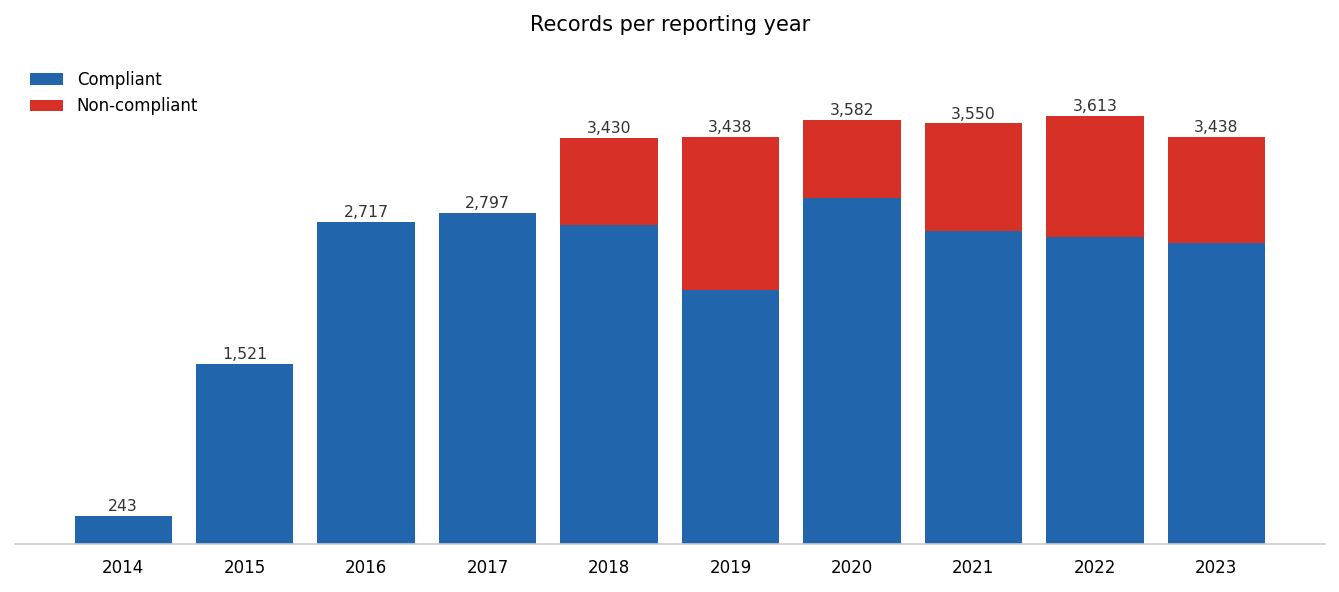
\includegraphics[width=0.85\linewidth]{figures/fig_01_records_per_year.png}
\caption*{\textbf{Figure 4.1. Dataset coverage by reporting year, stacked by compliance status.} Records grew steeply from 2014 to 2018 as the programme was phased in, then stabilised at roughly 3,400--3,600 per year. Compliant records (blue) consistently outnumber non-compliant (red) in every year. Author's analysis of Chicago Energy Benchmarking data (\cit{citynd}{City of Chicago, n.d.}).}
\end{figure}

\par\medskip\noindent
{\small\itshape \textbf{Table 4.1. Variable inventory by SCM role.} Observation counts and null rates are the author's analysis of the Chicago Energy Benchmarking dataset (\cit{citynd}{City of Chicago, n.d.}; $n = 28{,}329$). District steam and district chilled water are predominantly null because most buildings are not physically connected to the district energy network; this absence is a property of the building's infrastructure, not of the compliance gate. $^\dagger$Chicago Energy Rating was introduced in 2018; records from 2014--2017 carry a blank value regardless of compliance, so the null count here reflects the introduction date rather than non-compliance.\par}
\nopagebreak\medskip\nopagebreak
{
\footnotesize
\setlength{\tabcolsep}{5pt}
\renewcommand{\arraystretch}{1.15}
\begin{longtable}{>{\raggedright\arraybackslash}p{\dimexpr 0.434\linewidth-2\tabcolsep\relax}>{\raggedright\arraybackslash}p{\dimexpr 0.136\linewidth-2\tabcolsep\relax}>{\raggedright\arraybackslash}p{\dimexpr 0.16\linewidth-2\tabcolsep\relax}>{\raggedright\arraybackslash}p{\dimexpr 0.136\linewidth-2\tabcolsep\relax}>{\raggedright\arraybackslash}p{\dimexpr 0.134\linewidth-2\tabcolsep\relax}}
\toprule
Variable & Type & SCM role & Observed & Null \\
\midrule
\endfirsthead
\toprule
Variable & Type & SCM role & Observed & Null \\
\midrule
\endhead
\bottomrule
\endlastfoot
\multicolumn{5}{l}{\textbf{Upstream selection variables $\mathbf{X}_s$}} \\[-2pt]
\specialrule{0.3pt}{3pt}{5pt}
\nopagebreak
Gross floor area\newline \code{gross\_floor\_area\_buildings\_sq\_ft} & Continuous & $X_s$ & 26,104\newline (92.2\%) & 2,225\newline (7.8\%) \\
Primary property type\newline \code{primary\_property\_type} & Categorical, 63 levels & $X_s$ & 24,075\newline (85.0\%) & 4,254\newline (15.0\%) \\
\midrule
\multicolumn{5}{l}{\textbf{Upstream non-selection variables $X_o$}} \\[-2pt]
\specialrule{0.3pt}{3pt}{5pt}
\nopagebreak
Year built\newline \code{year\_built} & Integer & $X_o$ & 23,297\newline (82.2\%) & 5,032\newline (17.8\%) \\
Number of buildings\newline \code{of\_buildings} & Integer & $X_o$ & 23,875\newline (84.3\%) & 4,454\newline (15.7\%) \\
Data year\newline \code{data\_year} & Integer & $X_o$ & 28,329\newline (100\%) & 0 \\
\midrule
\multicolumn{5}{l}{\textbf{Compliance gate}} \\[-2pt]
\specialrule{0.3pt}{3pt}{5pt}
\nopagebreak
Compliance indicator $C$\newline \code{reporting\_status} + \code{exempt\_from\_chicago\_energy\_rating} & Binary & $C$ & 28,329\newline (100\%) & 0 \\
\midrule
\multicolumn{5}{l}{\textbf{Energy mediators $M^{\text{obs}}$}} \\[-2pt]
\specialrule{0.3pt}{3pt}{5pt}
\nopagebreak
Electricity use\newline \code{electricity\_use\_kbtu} & Continuous (kBtu) & $M^{\text{obs}}$ & 23,013\newline (81.2\%) & 5,316\newline (18.8\%) \\
Natural gas use\newline \code{natural\_gas\_use\_kbtu} & Continuous (kBtu) & $M^{\text{obs}}$ & 21,535\newline (76.0\%) & 6,794\newline (24.0\%) \\
District steam use\newline \code{district\_steam\_use\_kbtu} & Continuous (kBtu) & $M^{\text{obs}}$ (struct. zero) & 5,760\newline (20.3\%) & 22,569\newline (79.7\%) \\
District chilled water use\newline \code{district\_chilled\_water\_use\_kbtu} & Continuous (kBtu) & $M^{\text{obs}}$ (struct. zero) & 5,922\newline (20.9\%) & 22,407\newline (79.1\%) \\
Other fuel use\newline \code{all\_other\_fuel\_use\_kbtu} & Continuous (kBtu) & $M^{\text{obs}}$ & 82\newline (0.3\%) & 28,247\newline (99.7\%) \\
\midrule
\multicolumn{5}{l}{\textbf{Derived outcomes $Y^{\text{obs}}$}} \\[-2pt]
\specialrule{0.3pt}{3pt}{5pt}
\nopagebreak
Total GHG emissions\newline \code{total\_ghg\_emissions\_metric\_tons\_co2e} & Continuous (t CO$_2$e) & $Y^{\text{obs}}$ (target) & 21,714\newline (76.6\%) & 6,615\newline (23.4\%) \\
Site EUI\newline \code{site\_eui\_kbtu\_sq\_ft} & Continuous (kBtu/sq ft) & $Y^{\text{obs}}$ (derived) & 22,870\newline (80.7\%) & 5,459\newline (19.3\%) \\
Source EUI\newline \code{source\_eui\_kbtu\_sq\_ft} & Continuous (kBtu/sq ft) & $Y^{\text{obs}}$ (derived) & 22,011\newline (77.7\%) & 6,318\newline (22.3\%) \\
GHG intensity\newline \code{ghg\_intensity\_kg\_co2e\_sq\_ft} & Continuous (kg/sq ft) & $Y^{\text{obs}}$ (derived) & 21,709\newline (76.6\%) & 6,620\newline (23.4\%) \\
ENERGY STAR score\newline \code{energy\_star\_score} & Integer (1--100) & $Y^{\text{obs}}$ (derived) & 19,637\newline (69.3\%) & 8,692\newline (30.7\%) \\
Chicago Energy Rating\newline \code{chicago\_energy\_rating} & Ordinal (0--4 stars) & $Y^{\text{obs}}$ (special) & 19,406\newline (68.5\%) & 8,923\newline (31.5\%)$^\dagger$ \\
\end{longtable}
}
\par\medskip

Before the analysis proceeds, three features of Table 4.1 warrant comment.

\textbf{Upstream variables are partially observed.} The five upstream building characteristics are not fully observed: floor area is missing in 7.8\% of records, property type in 15.0\%, year built in 17.8\%, and number of buildings in 15.7\%. This is not a compliance-gate effect: upstream variables are drawn from the city building registry and carry missingness from registration gaps and data entry. Both compliant and non-compliant records contribute to these gaps equally, confirming that the missingness is independent of whether a building filed its EPA report.

\textbf{The compliance rate and the GHG observation rate are not the same.} Of 28,329 records, 22,819 (80.5\%) are compliant ($C = 1$) and 5,510 (19.5\%) are non-compliant ($C = 0$), while 21,714 (76.6\%) carry an observed GHG value. These three rates do not coincide, and the gaps are informative. Among the 22,819 compliant records, 21,406 have an observed GHG value and 1,413 do not: a building that filed under a status of ``Submitted'' may still lack a GHG figure if the submission was partial or failed the EPA platform's completeness checks. Among the 5,510 non-compliant records, the mirror case appears: 5,202 have no GHG value, as expected when no full report was filed, but 308 do, likely buildings that reported in some years and not others. The compliance gate therefore explains most but not all of the missingness in the outcome; the residual reflects reporting-side discrepancies in both directions.

\textbf{Chicago Energy Rating is not simply gated at the GHG rate.} The rating was introduced in 2018. Records from 2014--2017 (7,278 records, the first four reporting years) carry a blank rating by construction, regardless of compliance status. From 2018 onward, non-compliant buildings receive a rating of 0 by institutional mandate (\cit{cityndb}{City of Chicago, n.d.b}); compliant buildings receive 1--4 stars based on their ENERGY STAR score. Its overall null rate of 31.5\% therefore reflects the programme's introduction date, not the compliance-gate pattern that governs the other derived outcomes.

The dataset comes from Chicago's mandatory energy benchmarking programme; \code{reporting\_status} records whether a building met its obligation in a given year and is the basis for the compliance indicator $C$. Which buildings are obliged to report, the selection rule itself, is not assumed here; it is read from the governing documents in Stage 3 (Section 4.4). What the data show on their own is that compliance tracks building size: compliant buildings are systematically larger, with a median floor area of 131,000 sq ft against 92,966 sq ft for non-compliant records (Figure 4.2), and the compliant share rises across size bands. The 23.4\% gap in GHG coverage is therefore not a data-quality problem to be imputed away but a structural feature of which buildings the programme records, associated with an observed upstream characteristic.

\begin{figure}[tbp]
\centering
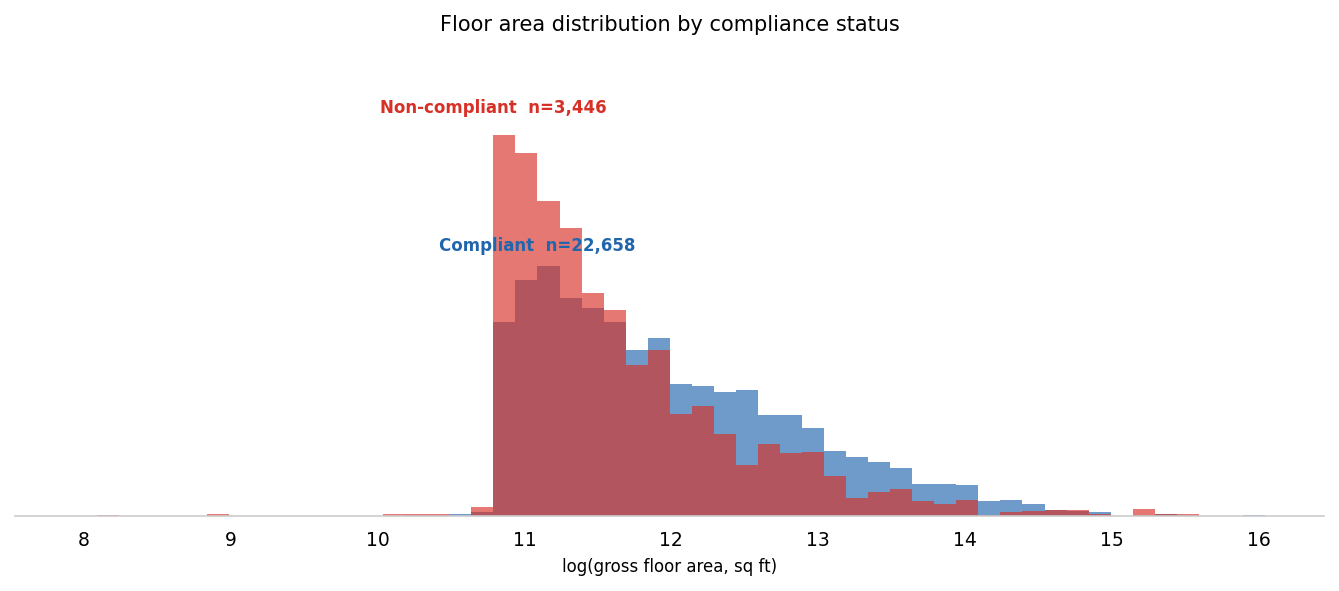
\includegraphics[width=0.72\linewidth]{figures/fig_05_floor_area_by_compliance.png}
\caption*{\textbf{Figure 4.2. Floor area distribution for compliant and non-compliant buildings.} Restricted to the 26,104 records with an observed floor area (compliant $n = 22{,}658$, non-compliant $n = 3{,}446$); floor area is null for the remainder, disproportionately among non-compliant records. Compliant buildings are systematically larger: the compliant median (131,000 sq ft) is 41\% larger than the non-compliant median (92,966 sq ft), and the two distributions diverge with size, though they overlap. Building size is the clearest correlate of compliance in the data. Author's analysis of Chicago Energy Benchmarking data (\cit{citynd}{City of Chicago, n.d.}).}
\end{figure}

The target variable spans five orders of magnitude (Figure 4.3): minimum 0, median 1,026, maximum 185,162 metric tons CO$_2$e (mean 2,493, std 5,995). The distribution is severely right-skewed (the mean is 2.4 times the median), which reflects the multiplicative relationship between building size and emissions: a building twice as large emits roughly twice as much GHG. On the log$_{1+}$ scale the distribution is approximately Normal. The data record 63 property types, reflecting the heterogeneity of Chicago's building stock; 56 appear among the compliant records, 55 among the subset of those that carry an observed GHG value, which Section 5 uses as the compliant training set (Figure 4.4): multifamily housing dominates (11,278 records), followed by K-12 schools (3,503) and offices (3,214). Prior work on benchmarking prediction uses the observed compliant sample directly, without accounting for the compliance gate that produced it (\cit{hsu2015}{Hsu, 2015}; \cit{kontokostatull2017}{Kontokosta \& Tull, 2017}).

\begin{figure}[tbp]
\centering
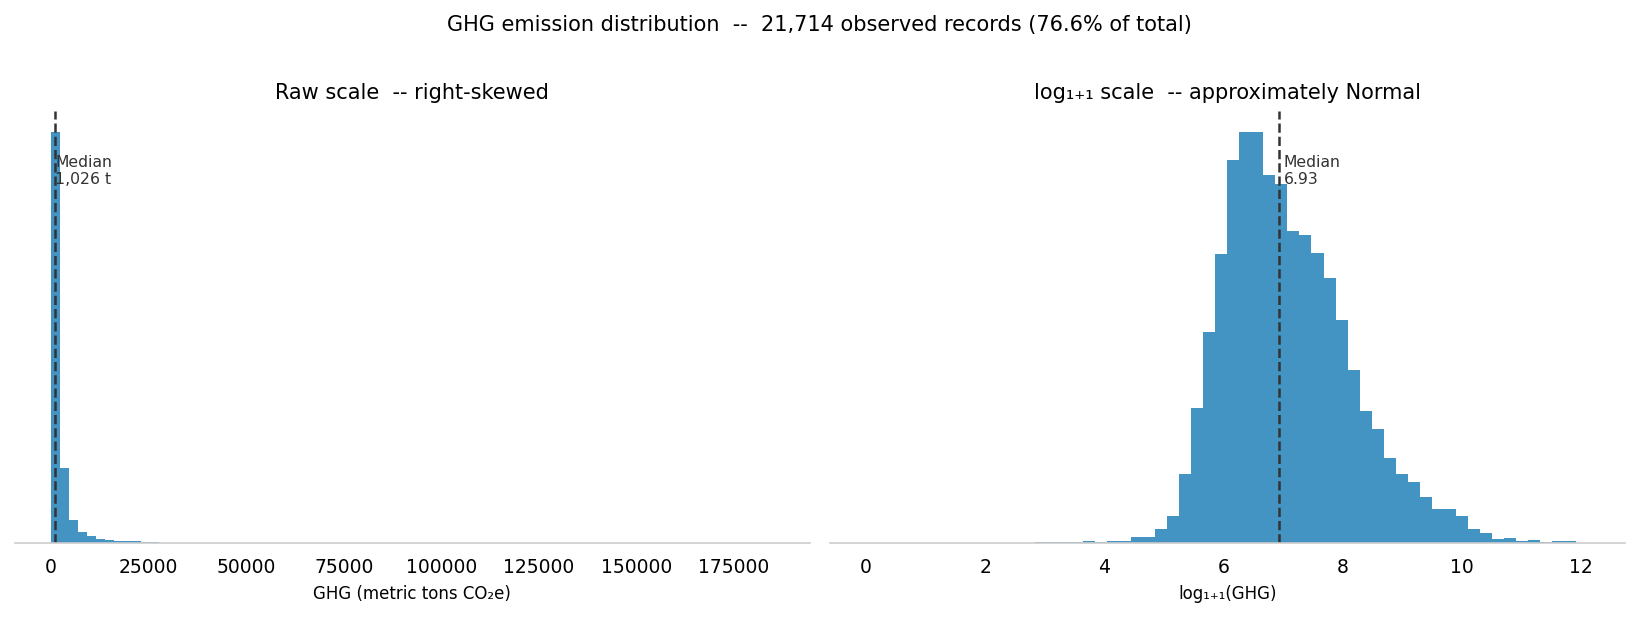
\includegraphics[width=0.86\linewidth]{figures/fig_02_ghg_distribution.png}
\caption*{\textbf{Figure 4.3. GHG emission distribution on raw and log$_{1+}$ scale (observed records only, $n = 21{,}714$).} The raw distribution is severely right-skewed: the mean (2,493 t) is 2.4$\times$ the median (1,026 t), and the largest building emits 180$\times$ the median building. The log$_{1+}$ transformation produces a distribution close to Normal. Author's analysis of Chicago Energy Benchmarking data (\cit{citynd}{City of Chicago, n.d.}).}
\end{figure}

\begin{figure}[tbp]
\centering
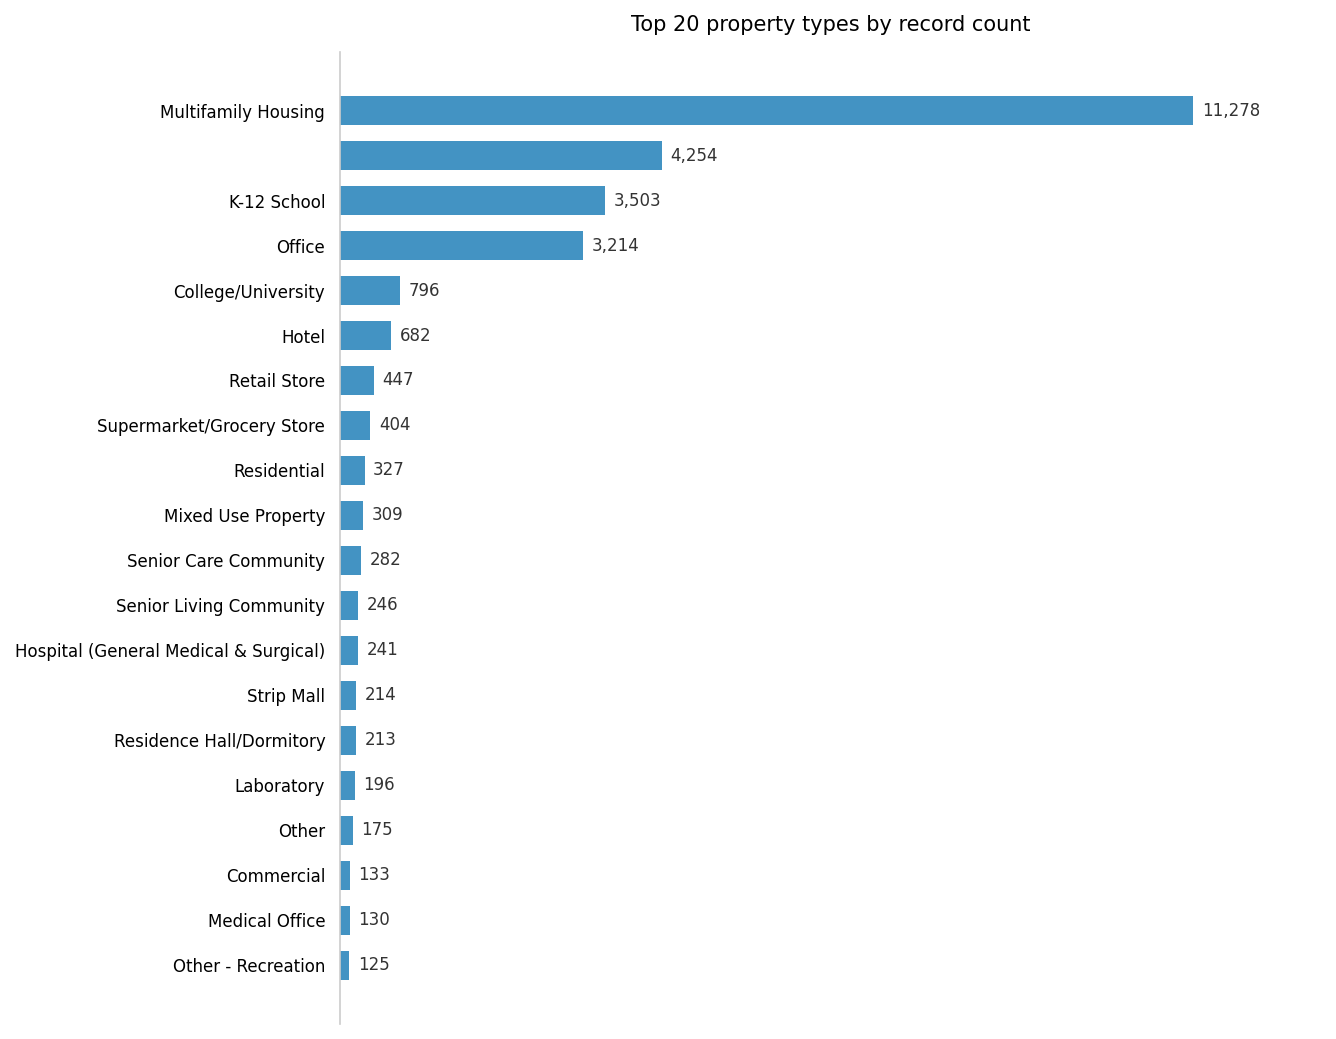
\includegraphics[width=0.58\linewidth]{figures/fig_07_property_type_frequency.png}
\caption*{\textbf{Figure 4.4. Top 20 property types by record count (all 28,329 records).} Multifamily housing accounts for 40\% of all records; the dataset is dominated by residential buildings and public-sector facilities (schools, universities). The bar for missing property type (4,254 records) shows buildings whose type is not recorded in the city registry. Author's analysis of Chicago Energy Benchmarking data (\cit{citynd}{City of Chicago, n.d.}).}
\end{figure}


\subsection{Stage 1 Applied: The Shadow Matrix}

Stage 1 reads the recording layer from the data alone, before any governing document is opened. It needs two things: the compliance indicator $C$ and the structure of co-missingness across the file. The compliance indicator is read, not imputed: $C = 1$ when \code{reporting\_status} is \code{Submitted} or \code{Submitted Data} and the building is not exempt from the Chicago Energy Rating, and $C = 0$ otherwise. The exemption flag is null-filled to false, the conservative reading, since a missing exemption is treated as no exemption. This yields 22,819 compliant records (80.5\%) and 5,510 non-compliant (19.5\%). Because $C$ is observed for every record ($C \in \mathcal{O}$), it can anchor the correlation analysis without itself being subject to missingness.

The obvious first look is the per-variable missing rate (Figure 4.5), and it is the wrong instrument. The most-missing fields are water use (85.7\%) and district steam and chilled water (79.7\%, 79.1\%), yet these are not the gated block. Their blanks are structural: most buildings are not connected to the district energy network, as Section 4.1 noted. The gated outcome and mediator fields sit far lower, clustered near the 23.4\% outcome-missing line: GHG and its intensity (23.4\%), the energy-use intensities (19.3\% to 23.2\%), electricity (18.8\%), and natural gas (24.0\%). A raw rate cannot separate a structural absence from a gate. For that, Stage 1 turns from the rate of missingness to its correlation structure.

\begin{figure}[tbp]
\centering
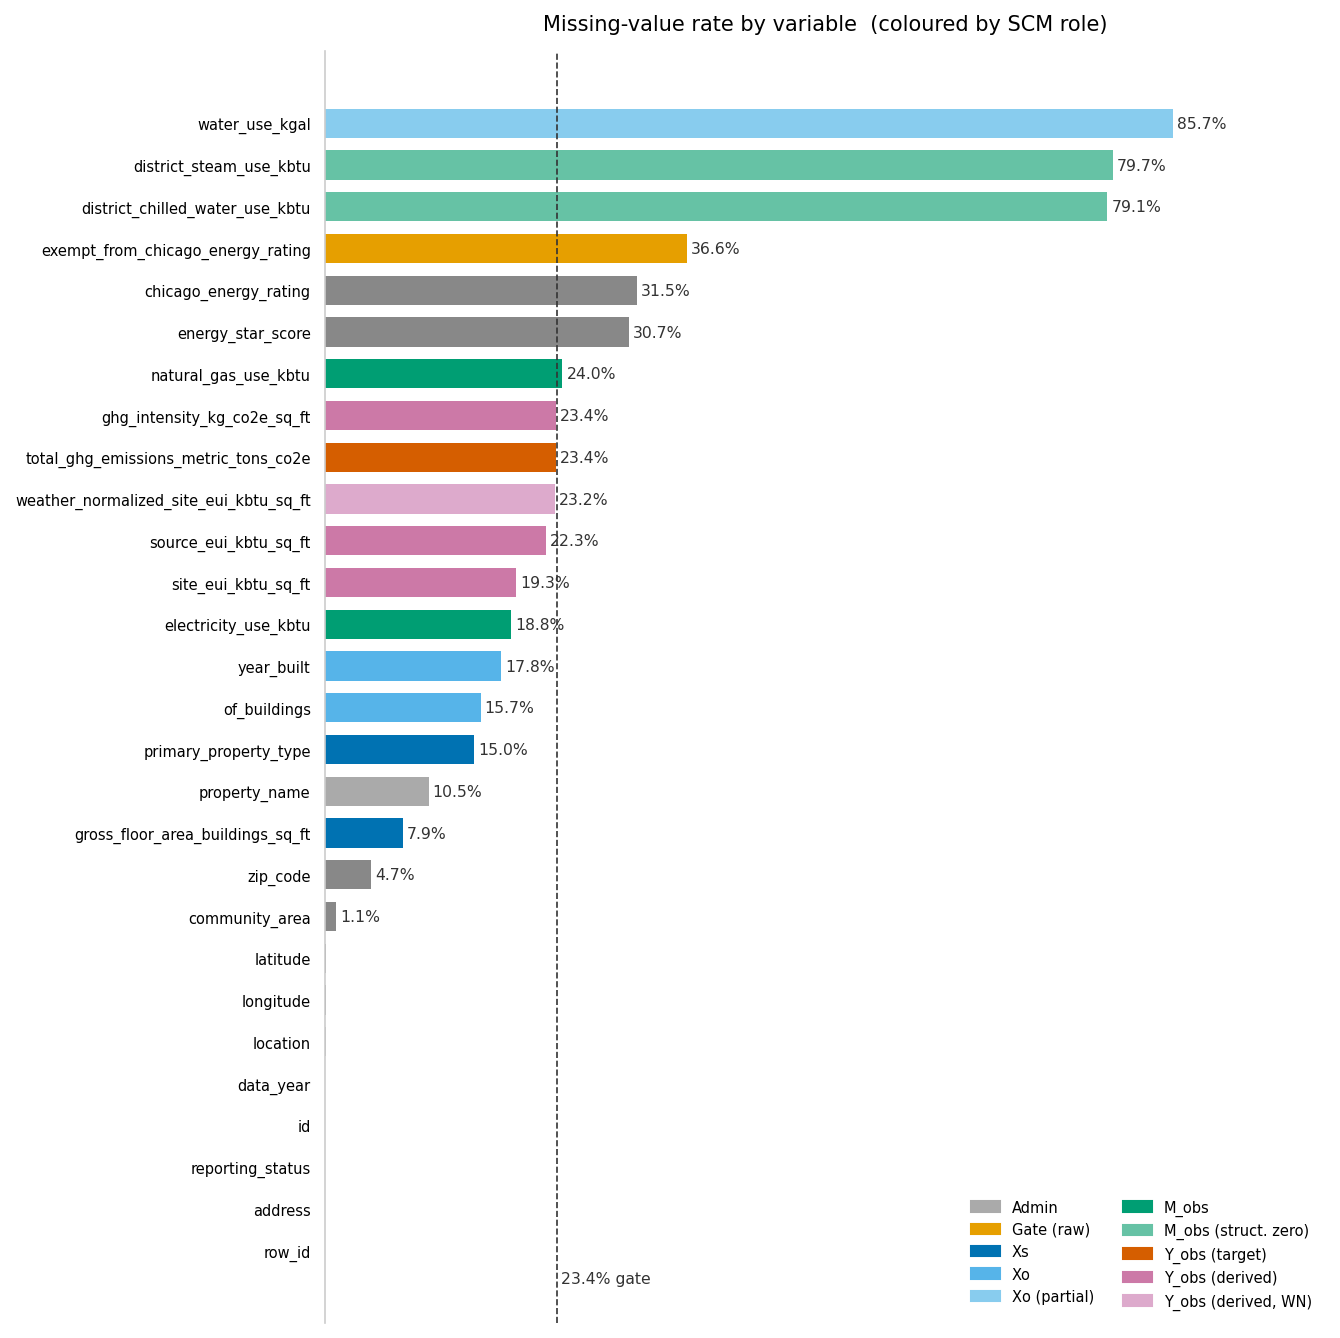
\includegraphics[width=0.80\linewidth]{figures/fig_03_missingness_by_variable.png}
\caption*{\textbf{Figure 4.5. Missing-value rate by variable, coloured by SCM role.} The most-missing fields (water use, district steam and chilled water) are structural absences, not gated fields; the gated mediators and outcomes cluster near the 23.4\% outcome-missing line (dashed). Raw missingness rate does not distinguish a structural zero from a compliance gate. Author's analysis of Chicago Energy Benchmarking data (\cit{citynd}{City of Chicago, n.d.}).}
\end{figure}

The shadow matrix (Figure 4.6) is the matrix of pairwise correlations among the variables' observation indicators, with $C$ appended. The three regimes of Section 3.1 are directly visible. \textbf{Gate alignment:} the gated mediators and derived outcomes correlate strongly with $C$: electricity 0.93, site EUI 0.91, source EUI 0.84, GHG, GHG intensity and weather-normalised EUI 0.83, natural gas 0.80, ENERGY STAR score 0.73. Each field is observed almost exactly when the building complied. \textbf{Block structure:} within that set the observation indicators co-vary between 0.74 and 1.00 (mean 0.88); electricity and site EUI move together at 0.98, and GHG and GHG intensity at 1.00. The fields appear and vanish as a single unit, the fingerprint of an atomic reporting gate (Condition 3 of Definition 2.1). \textbf{Idiosyncratic missingness:} present too, but confined outside the gated block. The geographic coordinates (latitude, longitude, location) correlate near zero with $C$ and with every substantive field ($|r| \approx 0.02$); their blanks carry no information about compliance. The three share a single geocoding source and so co-miss in one small block (15 records, 0.1\%) rather than scattering at random, but the property that matters holds: the shadow matrix sets them cleanly apart from the gate-driven block, which is the discrimination the diagnostic exists to provide.

\begin{figure}[tbp]
\centering
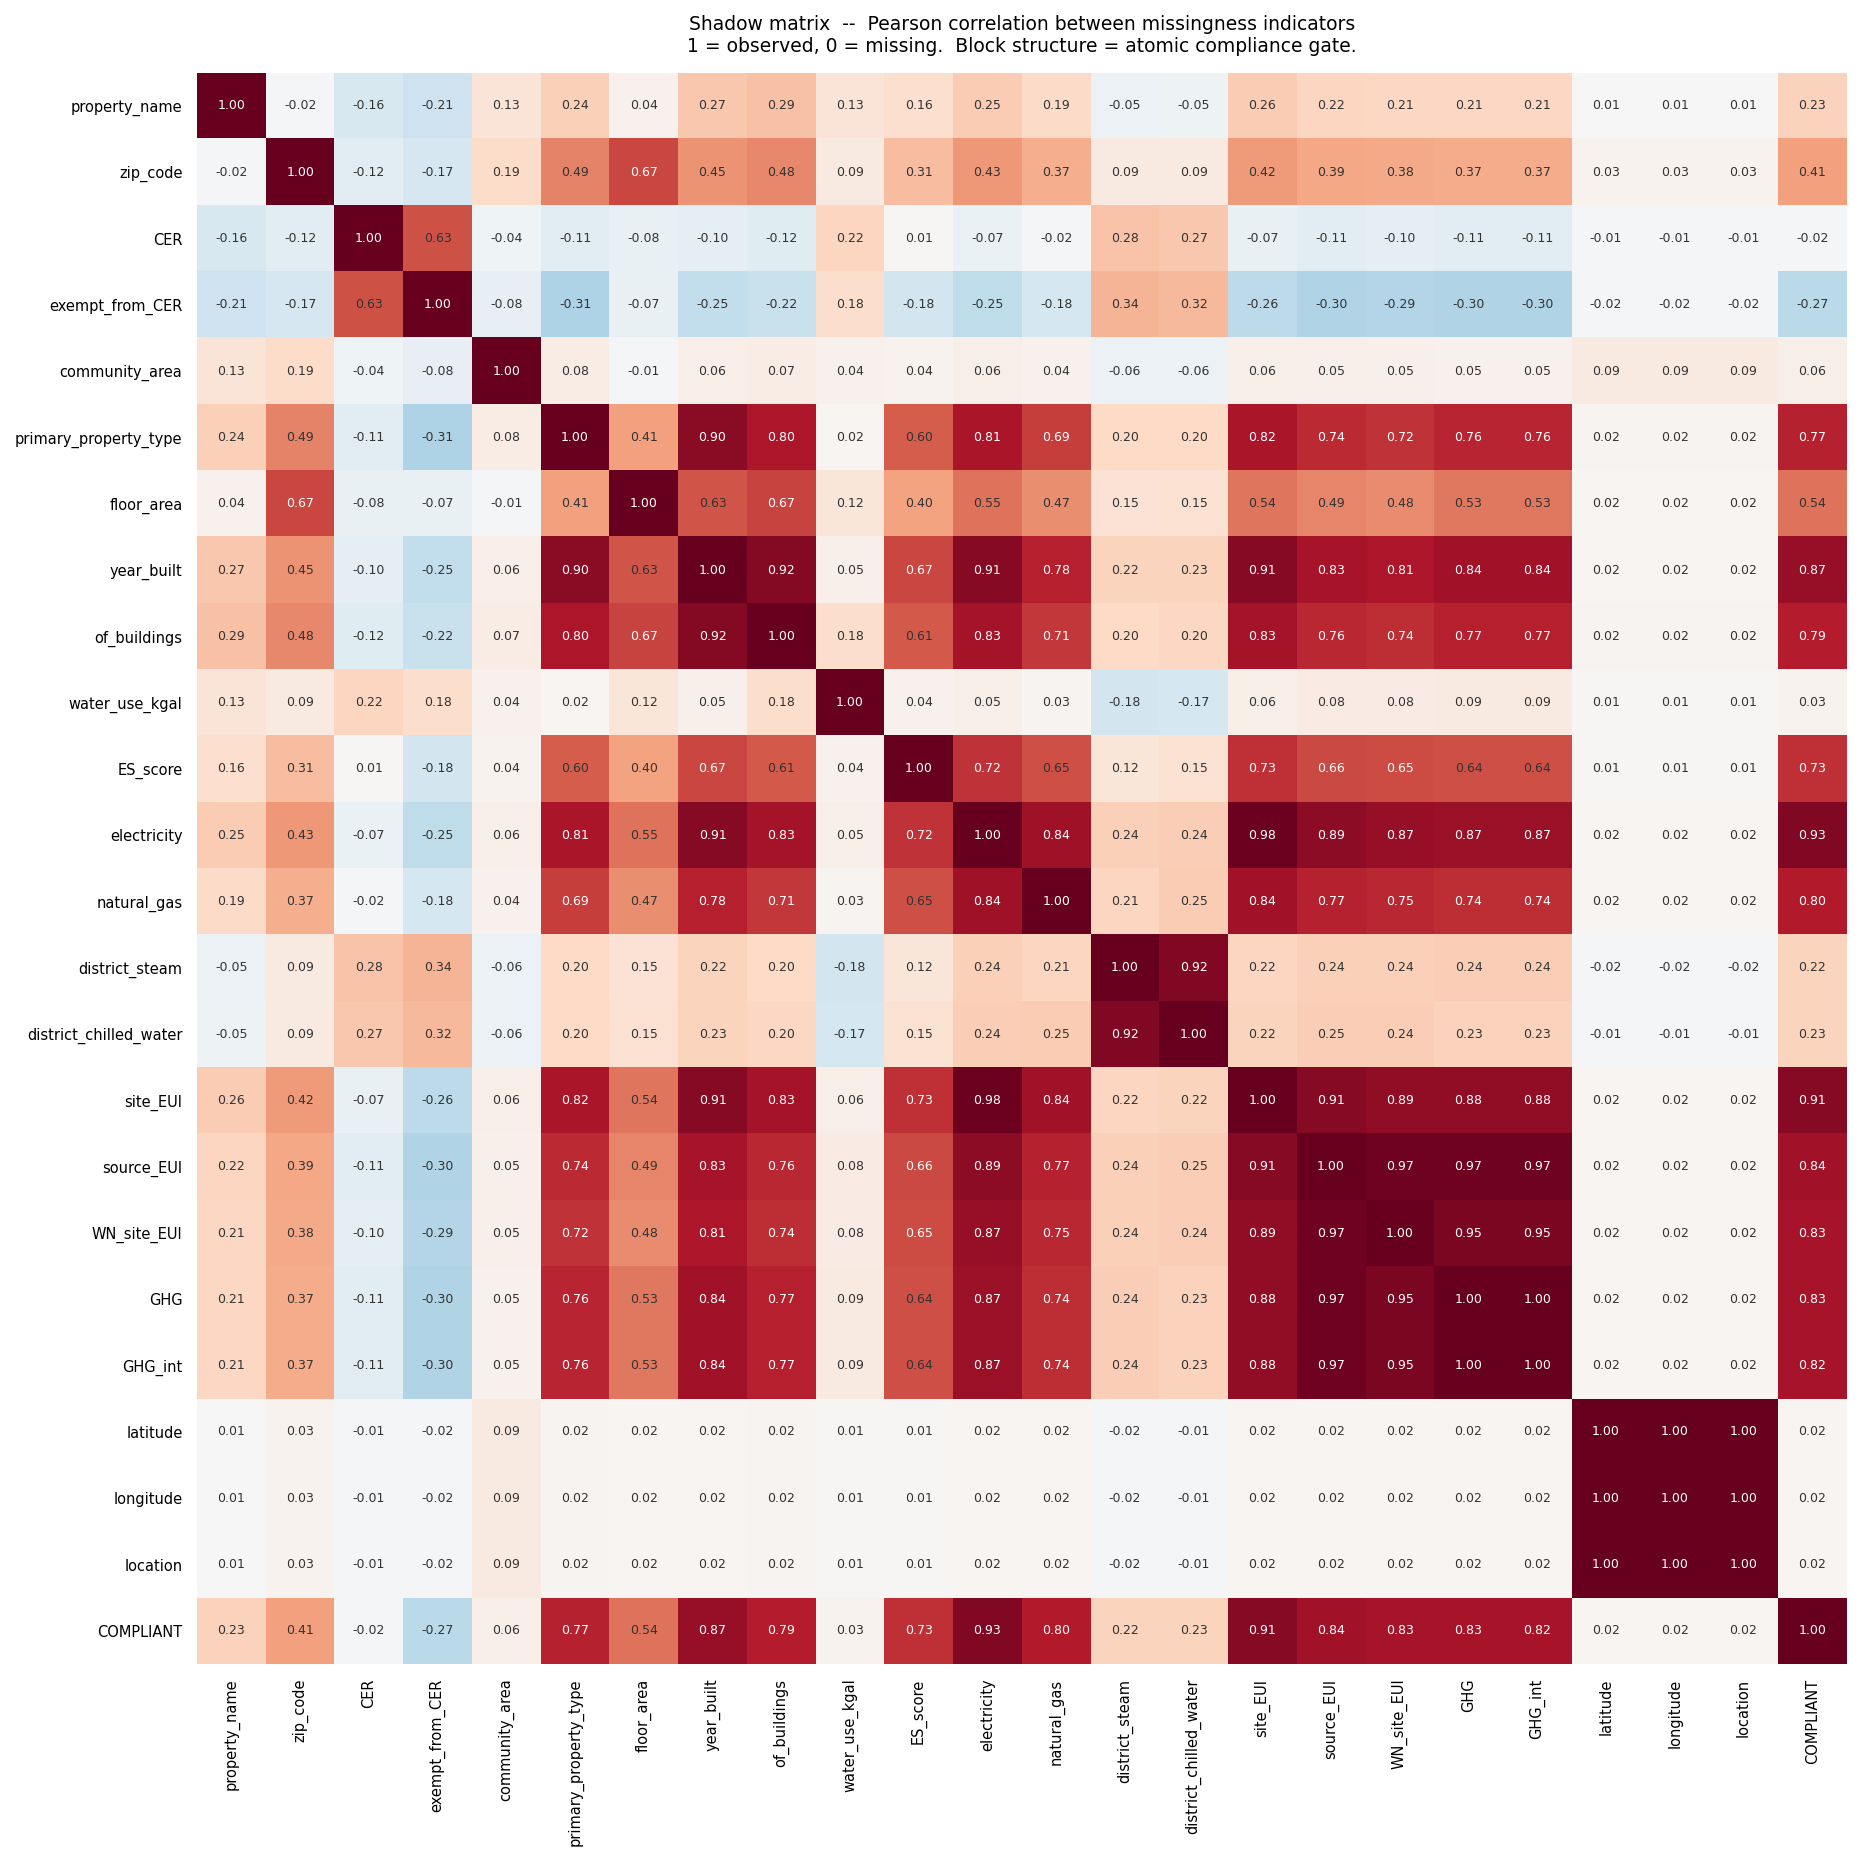
\includegraphics[width=0.80\linewidth]{figures/fig_04_shadow_matrix.png}
\caption*{\textbf{Figure 4.6. Shadow matrix: correlations among observation indicators.} Each cell is the correlation between two fields' missingness, with the compliance indicator appended. The gated mediators and derived outcomes form a dark block that also aligns with compliance; structural zeros, the Chicago Energy Rating, and the upstream and spatial fields sit outside it. Author's analysis of Chicago Energy Benchmarking data (\cit{citynd}{City of Chicago, n.d.}).}
\end{figure}

Three groups sit apart from the gated block, exactly as Section 3.1 anticipates, and reading them out is as much of Stage 1 as identifying the block itself. \textbf{Structural zeros:} district steam and chilled water correlate only 0.22 and 0.23 with $C$. Their blanks track the building's physical configuration, not the gate, and must be preserved as genuine zeros rather than recoded as gated missing. \textbf{The Chicago Energy Rating anomaly:} the rating correlates $-0.02$ with $C$, effectively not at all. Its missingness is governed by the programme's 2018 introduction date rather than compliance, so despite being a performance field it does not belong to the gated block. \textbf{Upstream fields:} floor area, property type, year built and number of buildings correlate with $C$ only moderately and unevenly (0.54 to 0.87); their missingness reflects registry completeness, a separate mechanism Section 4.1 already flagged, so Stage 1 leaves them outside the gated block. Among the spatial fields, only the ZIP code carries a compliance signal (0.41, tracking building size rather than compliance directly); community area and the coordinates carry essentially none.

The block-and-gate pattern is incompatible with data missing completely at random, under which every off-diagonal correlation would be zero (\cit{littlerubin2002}{Little \& Rubin, 2002}). Refuting that hypothesis rules out the default workflows, complete-case analysis and unconditional imputation, and forces the structural treatment that follows. Stage 1's output is a map of the observation structure, established from the data alone and independently of the documents Stage 3 will test against: the gate $C$; the gated block $\{M^{\text{obs}}, Y^{\text{obs}}\}$ of energy mediators and derived performance fields; the structural zeros to be preserved; and the upstream and spatial fields, whose lighter missingness is registry- or geocoding-driven and unrelated to the gate. The map stops at this partition. It shows the gated fields moving as one block but cannot, from co-missingness alone, separate the outcome within that block from the mediators that produce it. That separation is the work of Stage 2.


\subsection{Stage 2 Applied: The Candidate DAG}

Stage 2 turns the Stage 1 map into a candidate causal graph of the world layer that generated the Chicago data. The materials are deliberately limited to the shadow matrix, the variable descriptions, and Definition 2.1; the benchmarking ordinance and the EPA accounting standard stay closed until Stage 3, so the graph and the documents that will test it remain independent. The five-step procedure of Section 3.2 applies directly; Figure 4.7 shows the candidate DAG it produces.

\begin{figure}[H]
\centering
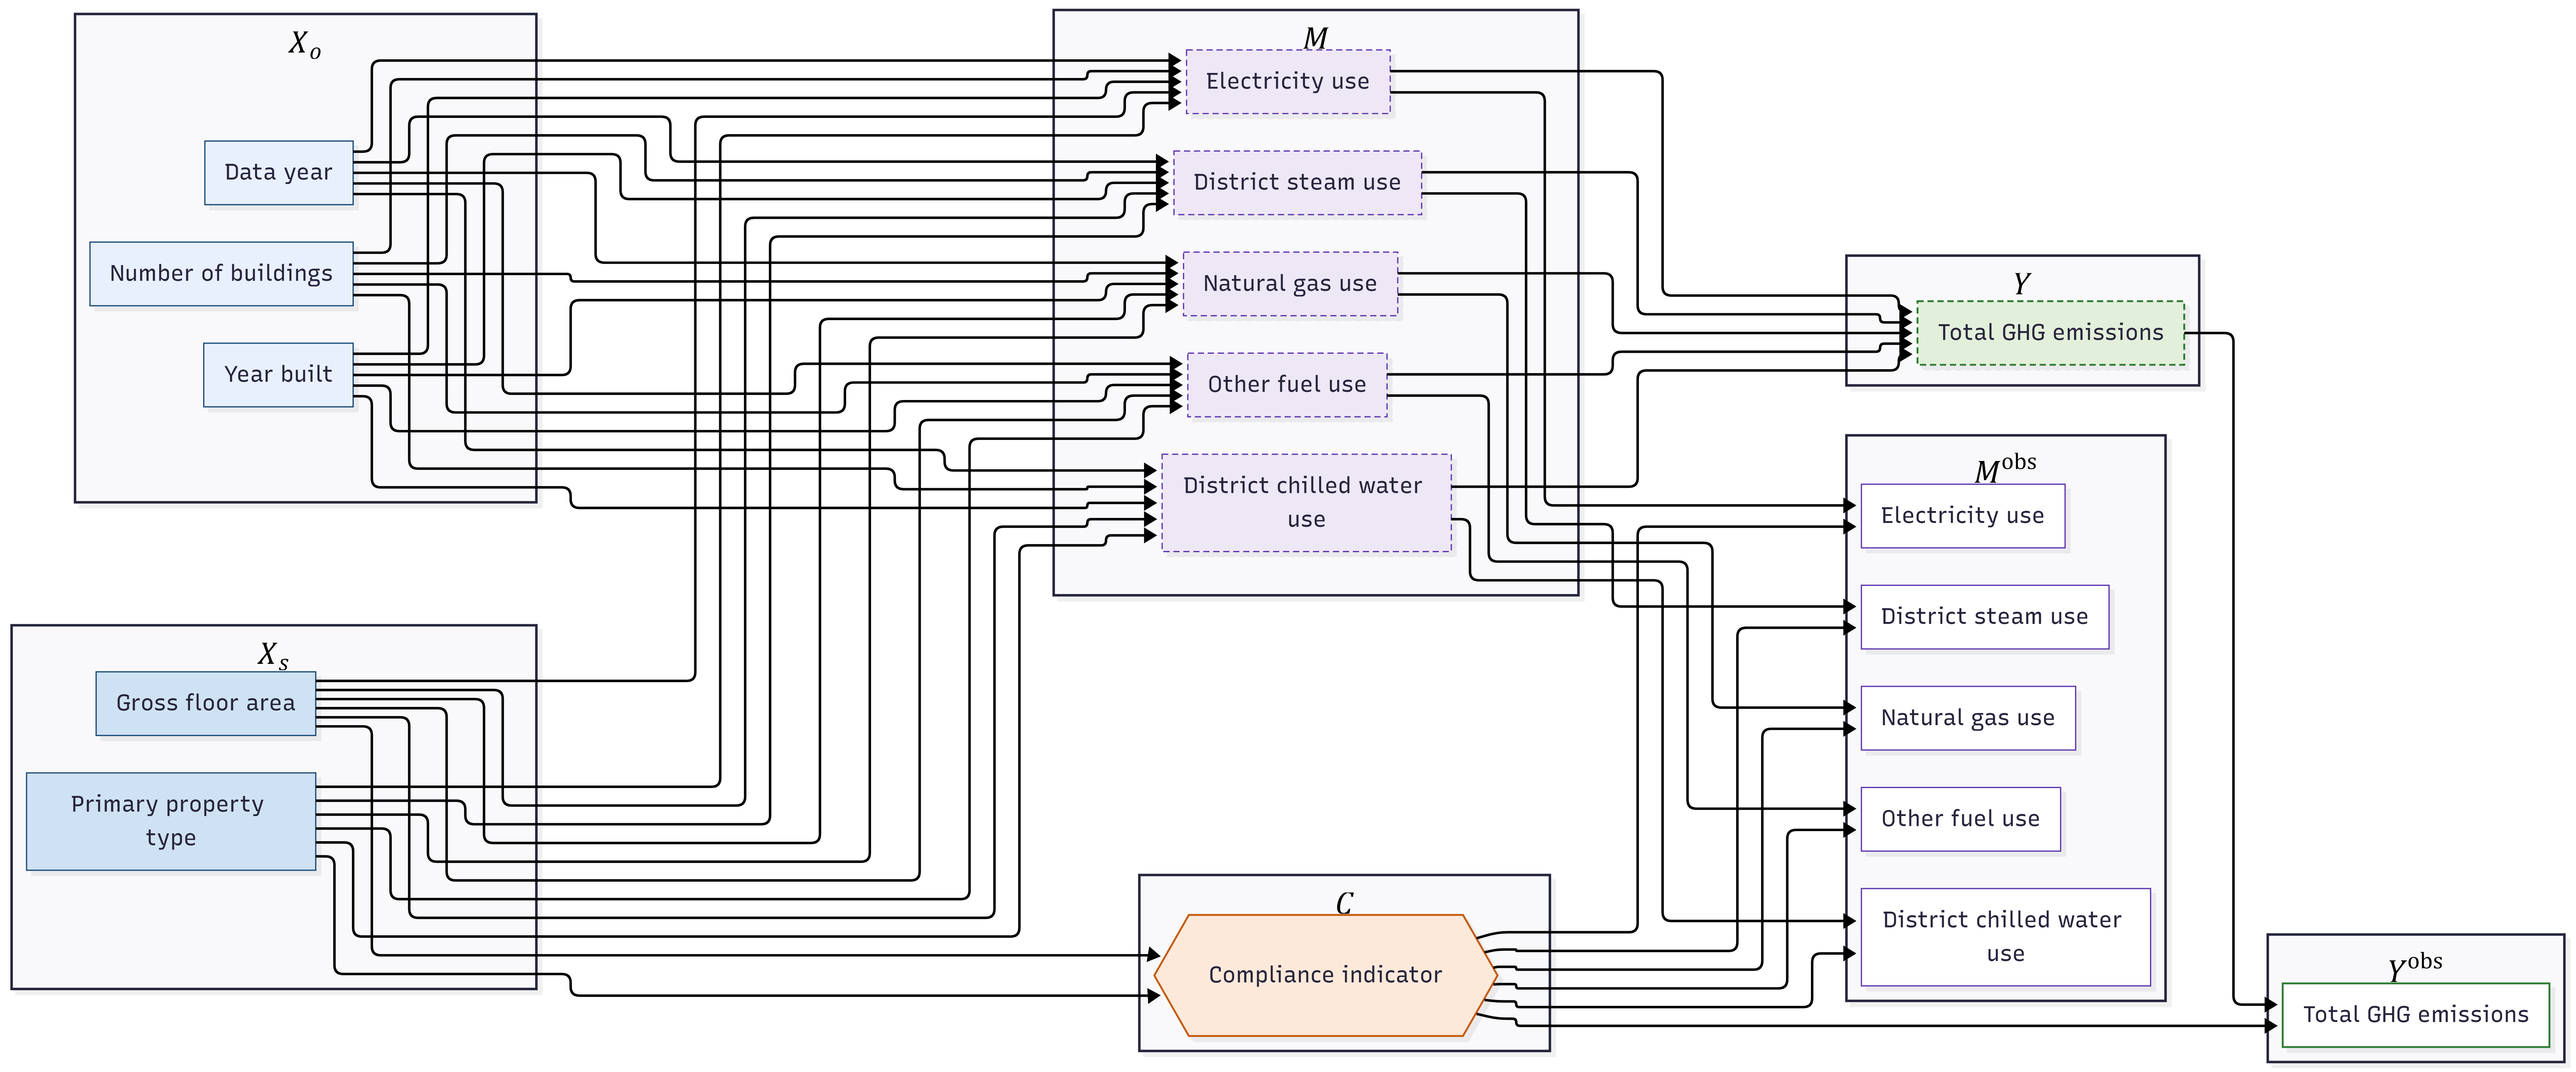
\includegraphics[width=0.98\linewidth]{figures/figure4_7.png}
\caption*{\textbf{Figure 4.7. Candidate DAG for the Chicago data (Stage 2 output).} The Definition 2.1 template instantiated with the Chicago variables, one node per variable. The selection variables $\mathbf{X}_s$ (gross floor area, primary property type) cause the compliance gate $C$ and, with the non-selection features $X_o$ (year built, number of buildings, data year), the latent energy mediators $M$ (electricity, natural gas, district steam, district chilled water, other fuel use); the mediators produce the latent outcome $Y$ (total GHG emissions). The gate $C$ governs the recorded layers $M^{\text{obs}}$ and $Y^{\text{obs}}$: each recorded field equals its latent value when $C = 1$ and is missing otherwise (the colliders $M \to M^{\text{obs}} \leftarrow C$ and $Y \to Y^{\text{obs}} \leftarrow C$). Latent nodes are dashed. Author's construction from the shadow matrix, variable descriptions, and Definition 2.1.}
\end{figure}

\textbf{Step 1. Carry over the partition (data).} From Stage 1: the gate $C$ is fixed; the gated block $\{M^{\text{obs}}, Y^{\text{obs}}\}$ holds the metered energy fields and the derived performance fields that co-miss with $C$; the structural zeros (district steam, district chilled water) are flagged as physical absences to preserve; and the upstream set holds the building characteristics, whose lighter missingness is unrelated to the gate. The shadow matrix shows the gated block as one undifferentiated group: it cannot, on its own, tell the outcome within it from its mediators (Section 4.2).

\textbf{Step 2. Name the outcome $Y$ (choice).} The research question fixes $Y$ as total GHG emissions (\code{total\_ghg\_emissions\_metric\_tons\_co2e}), the quantity the programme exists to measure. The other gated performance fields (the energy-use intensities, GHG intensity, and ENERGY STAR score) are further performance measures derived from the same mediators rather than the target; the graph admits them as a fan of co-outcomes (Section 3.2), but the study tracks total GHG.

\textbf{Step 3. Reason the mediators $M$ (conjecture).} Among the remaining gated fields, five metered energy quantities (electricity, natural gas, district steam, district chilled water, and other fuel use) are, by the descriptions, the channels through which a building's characteristics produce emissions. They are taken as the mediators $M$ feeding $Y$, giving the structural claim $\mathrm{pa}(Y) = M$. District steam and chilled water enter $M$ as structural zeros for buildings off the district network (Section 4.1). This separation of mediators from outcome is made by argument; the shadow matrix cannot perform it.

\textbf{Step 4. Reason the selection variables $\mathbf{X}_s$ (conjecture).} Within the upstream set, gross floor area is the feature the descriptions mark as a measure of building size, the kind of eligibility criterion a threshold gates on (Condition 1), and primary property type is a categorical eligibility criterion of the same kind. They are taken as $\mathbf{X}_s$; year built and number of buildings are $X_o$, upstream causes of energy use that play no part in selection, alongside the data year, a yearly fixed effect that captures annual variation in energy consumption (weather, prices, code changes) rather than a building characteristic. The data corroborate the floor-area conjecture: compliant buildings are scarce at small sizes and predominate as size grows (Figure 4.2), consistent with floor area as the selection variable. Realized compliance is not perfectly sharp, so the signature is suggestive, not decisive, and speaks only to selection; whether the documented rule actually reads floor area and property type is reserved for Stage 3.

\textbf{Step 5. Instantiate the edges (template).} With the roles assigned, Definition 2.1 supplies every edge with no further argument: $\mathbf{X}_s \to C$, $\mathbf{X}_s \to M$ and $X_o \to M$, $M \to Y$, and the institution layer $M \to M^{\text{obs}} \leftarrow C$ with $Y \to Y^{\text{obs}} \leftarrow C$. The result is Figure 2.1's template with each role expanded into its Chicago variables (Figure 4.7).

The candidate DAG makes three predictions that Stage 3 will set against the documents:

\begin{enumerate}
  \item \textbf{P1 (selection):} compliance is caused by the upstream characteristics $\mathbf{X}_s$, not by energy use or emissions; the gate reads building size and type, nothing downstream.
  \item \textbf{P2 (atomic gate):} the mediators and the outcome are observed or withheld as a single unit governed by $C$, a prediction the shadow-matrix block of Section 4.2 already corroborates in the data.
  \item \textbf{P3 (mediator sufficiency):} $\mathrm{pa}(Y) = M$, so total emissions are a function of the metered energy mediators alone, with no direct parent outside $M$.
\end{enumerate}

P3 is the sharpest and least supported claim. Nothing in the shadow matrix, which cannot separate the outcome from its mediators inside the gated block, can establish it; it rests for now on the variable descriptions alone. Stage 3 tests it against the EPA accounting standard that fixes how emissions are computed from metered energy, and tests the selection and classification claims against the ordinance (Section 4.4).


\subsection{Stage 3 Applied: Falsification and Conformance}

Stage 3 tests the candidate DAG against documents that took no part in building it, so any clash would be genuine evidence against the graph rather than circular confirmation. The graph came from the shadow matrix, the variable descriptions, and Definition 2.1 alone (Section 4.3), while the benchmarking ordinance, the reporting schema, and the EPA accounting standard were held back for exactly this purpose. Set against the three predictions that close Section 4.3, none of these documents contradicts the graph.

The ordinance defines a building's duty to report by its size and property class, settling the selection prediction. Under the Municipal Code of Chicago, Chapter 18-14 (\cit{city2013}{City of Chicago, 2013}), a building is ``covered'' on two upstream characteristics only, a gross floor area at or above 50,000 square feet and a property class, with municipal, commercial, and residential buildings drawn in and named categories (stadiums, industrial and manufacturing facilities, storage and hazardous-material buildings) exempted. Covered owners must benchmark in ENERGY STAR Portfolio Manager and file each year. Floor area and property type are exactly the two variables Step 4 assigned to $\mathbf{X}_s$, and the duty turns on no energy or emissions quantity, which a building has not reported when its obligation is set. The phased rollout corroborates the same edge from a second direction: eligibility was extended by size and class over three cycles (commercial above 250,000 sq ft in 2014; commercial 50,000 to 250,000 and residential above 250,000 in 2015; residential 50,000 to 250,000 in 2016), and the record counts climb in step (Figure 4.1). Because the thresholds were switched on year by year, the same rollout also gives the data year a transient role in the gate, which the refinement below makes explicit.

A single annual Portfolio Manager submission carries every metered and derived field at once, so the atomic gate needs no separate document: the one-report obligation makes the whole block appear or vanish together. The shadow matrix already showed exactly this pattern in Stage 1 (Section 4.2).

The mediator/outcome split is the reporting schema's own, not the DAG's invention: a building enters site energy per fuel (electricity, natural gas, district steam, district chilled water, and minor others), and Portfolio Manager derives Total GHG Emissions, site and source EUI, and the ENERGY STAR score from those meters (\cit{epa2025}{U.S. EPA, 2025}). The five metered quantities are therefore $M$, total GHG is $Y$, and the remaining performance fields are the co-outcome fan, each a further function of the same meters rather than a parent of $Y$.

The accounting standard then makes the sufficiency claim itself explicit, computing emissions by ``multiplying the site energy for each fuel by the emissions factor for that specific fuel type'' and summing across fuels (\cit{epa2025}{U.S. EPA, 2025}), which is exactly the additive form $\mathrm{pa}(Y) = M$ requires:

\[
\mathrm{GHG} = \sum_{f} \phi_f\, E_f .
\]

Here $E_f$ is the site energy the building draws from fuel $f$ and $\phi_f$ is that fuel's emission factor, the sum running over the metered fuels. The standard fixes each $\phi_f$ as a published constant, a national value for each combustion and district fuel and a regional, year-specific eGRID factor for electricity (Table 4.2).

Because every $\phi_f$ is set outside the building, the standard makes $Y$ a deterministic function of the metered fuels, which is P3 in the institution's own terms: among building characteristics, none parents $Y$ except through the meters. Whether the recorded data actually obey the formula is a separate, quantitative question, taken up below.

The documentary comparison settles the structure; two data-side checks corroborate it where the data can speak: an outcome reconstruction (does $M$ recover $Y$?) and an upstream-to-mediator regression (does $X$ drive $M$?), both drawn from the full panel of 28,329 building-year records (2014--2023) and prepared as follows.

\begin{enumerate}
  \item \textbf{Reconstruction.} The 21,704 records with an observed GHG value and finite, non-negative energy (the energy filter removes 10 of the 21,714 GHG-observed records of Table 4.1); the regressors are the four metered fuels (electricity, gas, district steam, district chilled water), each unreported or off-network value set to zero, with other fuel (observed for 0.3\% of records) negligible and excluded.
  \item \textbf{Upstream regression.} Per mediator, the records with that mediator observed and all five upstream features present (floor area $> 0$).
  \item \textbf{Transforms.} The reconstruction is linear, since the documented accounting is additive; the upstream regression takes $\log(1+M)$ on $\log(\text{floor area})$ (so the coefficient is an elasticity), with year built and number of buildings entering linearly and property type and data year as fixed effects.
\end{enumerate}

Mediators are recorded only for the (largely) compliant units, so both fits sit on that subsample; conditioning on the upstream features that drive selection keeps $E[M \mid X]$ unbiased there.

Because the checks ask whether a connection exists and conforms, not what a coefficient is to three decimals, the tables report $R^2$ (decomposed by block), the full-model adjusted $R^2$ (to confirm the fit is not inflated by the parameter count), the floor-area elasticity, and the recovered emission factors. Standard errors and test statistics are omitted, since with $n$ in the tens of thousands they would be uniformly significant and would over-weight a check subordinate to the documentary test.

If $\mathrm{pa}(Y) = M$ and the recorded outcome implements the documented formula, total emissions must reconstruct as a near-exact linear combination of the metered fuels, so the first check fits that same identity to the records, now with a residual to absorb any departure:

\[
\mathrm{GHG}_i = \sum_{f \in \mathcal{F}} \phi_f\, E_{if} + \varepsilon_i ,
\qquad \mathcal{F} = \{\text{electricity, gas, steam, chilled water}\}.
\]

Here $\mathrm{GHG}_i$ and $E_{if}$ are the emissions and the fuel-$f$ energy recorded for building-year $i$, $\phi_f$ is the fitted factor for fuel $f$, $\mathcal{F}$ is the set of metered fuels, and $\varepsilon_i$ is the residual.

Because the electricity grid decarbonises year on year, we also fit a variant in which electricity carries a year-specific factor while the combustion fuels stay constant:

\[
\mathrm{GHG}_i = \sum_{t} \phi^{\text{elec}}_{t}\, \mathbf{1}\{\text{year}_i = t\}\, E_{i,\text{elec}} + \sum_{f \neq \text{elec}} \phi_f\, E_{if} + \varepsilon_i .
\]

Here $\phi^{\text{elec}}_t$ is a separate electricity factor for each data year $t$, $\mathbf{1}\{\text{year}_i = t\}$ selects the year of record $i$, and the combustion and district fuels keep the single factor $\phi_f$ of the first variant.

\par\medskip\noindent
{\small\itshape \textbf{Table 4.2. Recovered emission factors against the EPA standard.} For each metered fuel: the EPA-prescribed emission factor (\cit{epa2025}{U.S. EPA, 2025}) and the factor recovered by the no-intercept reconstruction above ($n = 21{,}704$). $^\ddagger$Electricity has no single EPA value, taking a year-specific regional eGRID factor (Chicago's RFCW subregion, 121.78 in 2023, higher earlier); the recovered 169.1 is the multi-year average (see text). Author's analysis of Chicago Energy Benchmarking data (\cit{citynd}{City of Chicago, n.d.}).\par}
\nopagebreak\medskip\nopagebreak
{
\setlength{\tabcolsep}{7pt}
\renewcommand{\arraystretch}{1.15}
\begin{longtable}{lrr}
\toprule
Fuel & EPA factor (kg CO$_2$e/MBtu) & Recovered factor \\
\midrule
\endfirsthead
\toprule
Fuel & EPA factor (kg CO$_2$e/MBtu) & Recovered factor \\
\midrule
\endhead
\bottomrule
\endlastfoot
Electricity & eGRID RFCW, annual$^\ddagger$ & 169.1 \\
Natural gas & 53.11 & 53.7 \\
District steam & 66.40 & 58.2 \\
District chilled water & 49.31--73.89 & 49.3 \\
\end{longtable}
}
\par\medskip

The reconstruction confirms that the recorded emissions follow the documented formula, in three respects.

\begin{enumerate}
  \item \textbf{$\mathrm{pa}(Y) = M$.} A constant factor per fuel reproduces almost all of emissions ($R^2 = 0.987$), and a year-specific electricity factor makes the fit essentially exact ($0.9999$, the adjusted $R^2$ identical at this $n$), with no role for a parent of $Y$ outside $M$.
  \item \textbf{The residual is a documented trend, not noise.} The $0.987 \to 0.9999$ gain is entirely electricity's factor falling year on year (201 to 132 kg CO$_2$e/MBtu over 2014--2022), the grid decarbonising toward the published 2023 RFCW value: the auditable disturbance $U_Y$ with a diagnosable cause.
  \item \textbf{The factors conform to the standard.} Natural gas matches almost exactly (53.7 against the EPA-prescribed 53.11), and district chilled water lands on the engine-driven-chiller value (49.3 against 49.31). District steam runs below the documented value (58.2 against 66.40), the few buildings on the district network leaving its coefficient noisy. Electricity has no single benchmark: its recovered 169.1 is the multi-year average of a factor declining year on year (Table 4.2 note).
\end{enumerate}

Selection bias exists only if the upstream features drive the mediators (Condition 2), so the second check must establish that edge from the data. Because the mediators are metered rather than computed, no document speaks to the edge; it can be corroborated only by association: we regress each mediator on the upstream features,

\[
\log(1 + M_{if}) = \beta_0 + \beta_A\, \log A_i + \sum_p \gamma_p\, \mathbf{1}\{\text{type}_i = p\} + \sum_t \delta_t\, \mathbf{1}\{\text{year}_i = t\} + \theta_1\, \text{built}_i + \theta_2\, \text{nbldg}_i + \varepsilon_{if} ,
\]

Here $M_{if}$ is the fuel-$f$ energy and $A_i$ the gross floor area of building-year $i$; the indicators $\mathbf{1}\{\cdot\}$ encode property type $p$ and data year $t$; $\text{built}_i$ and $\text{nbldg}_i$ are the year built and number of buildings; $\beta_A$ is the floor-area elasticity, reported from the full model, and $\beta_0, \gamma_p, \delta_t, \theta_1, \theta_2$ are the remaining coefficients, with residual $\varepsilon_{if}$.

We fit it in nested blocks (floor area; $+$ property type; $+$ the rest), recording $R^2$ after each, so the column-to-column gains in Table 4.3 give each block's contribution.

\par\medskip\noindent
{\small\itshape \textbf{Table 4.3. Upstream features as drivers of the mediators.} Nested OLS of $\log(1+M)$ adding one block at a time: floor area [$R^2$ (area)], $+$ property type [$R^2$ (+ type)], $+$ year built, number of buildings, and data year [$R^2$ (full)]; the column-to-column gains give each block's contribution, and $\beta_A$ is the floor-area elasticity from the full model. Adjusted $R^2$ (full) differs from $R^2$ (full) by at most 0.001, so the fit is not inflated by the parameter count. The last row totals the metered fuels. Author's analysis of Chicago Energy Benchmarking data (\cit{citynd}{City of Chicago, n.d.}).\par}
\nopagebreak\medskip\nopagebreak
{
\footnotesize
\setlength{\tabcolsep}{5pt}
\renewcommand{\arraystretch}{1.15}
\begin{longtable}{lrrrrrr}
\toprule
Mediator & $n$ & $R^2$ (area) & $R^2$ (+ type) & $R^2$ (full) & adj. $R^2$ (full) & $\beta_A$ \\
\midrule
\endfirsthead
\toprule
Mediator & $n$ & $R^2$ (area) & $R^2$ (+ type) & $R^2$ (full) & adj. $R^2$ (full) & $\beta_A$ \\
\midrule
\endhead
\bottomrule
\endlastfoot
Electricity & 22,724 & 0.467 & 0.544 & 0.567 & 0.567 & 1.03 \\
Natural gas & 21,253 & 0.045 & 0.123 & 0.183 & 0.182 & 0.76 \\
District steam & 5,677 & 0.000 & 0.408 & 0.811 & 0.810 & 0.03 \\
District chilled water & 5,837 & 0.092 & 0.224 & 0.769 & 0.768 & 0.46 \\
Total metered energy & 22,723 & 0.438 & 0.472 & 0.488 & 0.487 & 0.94 \\
\end{longtable}
}
\par\medskip

The regression shows that the upstream features do drive the mediators, in two patterns.

\begin{enumerate}
  \item \textbf{Size drives the dominant mediators.} For electricity and total energy $\beta_A \approx 1$ (doubling floor area roughly doubles energy), with floor area alone explaining 44--47\%, so $\mathbf{X}_s$ is genuinely among the causes of $M$ and the bias is real; $\beta_A \approx 1$ also confirms floor area and energy are on consistent units.
  \item \textbf{The others load on type, not size.} For natural gas and the district fuels, floor area alone explains little (each with $R^2$ (area) below 0.10); property type lifts natural gas from $0.05$ to $0.12$ and carries the district fuels (steam $0.00 \to 0.41$). Gas is system-dependent, and the district fuels are structural zeros whose presence tracks type and location.
\end{enumerate}

The two checks corroborate the structure without carrying its weight, for two reasons. First, a regression reveals association, not direction. Orientation comes from outside the data: $M \to Y$ from the documented formula, which computes emissions from energy, and $X \to M$ from physical and temporal order, since building characteristics precede and produce energy use. Second, neither check is load-bearing for the selection correction's validity, which rests on the documented gate and $\mathrm{pa}(Y) = M$; together they establish only that the connections exist and conform to the documented accounting.

The tests refine the graph as well as confirm it, but the core survives intact: $\mathrm{pa}(Y) = M$ holds to $R^2 = 0.9999$, no mediator is missing, and no building feature parents $Y$ except through the meters.

The refinement falls in one place, the data year, which Figure 4.7 filed among the non-selection features $X_o$ on the hypothesis that it was an ordinary upstream characteristic. Stage 3 overturns that: the data year is the panel's period index rather than a building feature, so the refined DAG lifts it out of the partition (Figure 4.8), where it gains two edges the $X_o$ reading had missed, while year built and number of buildings keep their single edge to $M$:

\begin{enumerate}
  \item \textbf{Data year to $Y$.} Beyond driving energy use (its $\to M$ edge), the data year also acts on the energy-to-emissions conversion: the reconstruction's residual is the eGRID electricity factor falling year on year (inference 2 above), a documented and exogenous influence on $Y$ that Figure 4.7 had absorbed into the disturbance $U_Y$.
  \item \textbf{Data year to $C$.} The phased rollout makes eligibility itself time-varying through 2017, as the threshold fell from 250,000 to 50,000 square feet by class, so the data year enters the gate during the phase-in and the candidate reading that kept it out of selection (Step 4) is corrected.
\end{enumerate}

A further change is to functional form rather than topology: the ordinance fixes $\mathbf{X}_s \to C$ as a sharp threshold at 50,000 square feet with a property-class exemption, not the smooth dependence the candidate edge left implicit.

None of this costs the analysis anything. The data year is observed for every record (Table 4.1) and is already conditioned on in both the propensity and outcome models, so the backdoor the new edges open, $C \leftarrow \text{data year} \rightarrow Y$, is already blocked; the edges only reclassify parts of $U_C$ and $U_Y$ as documented, observed causes. Figure 4.8 records the result.

\begin{figure}[H]
\centering
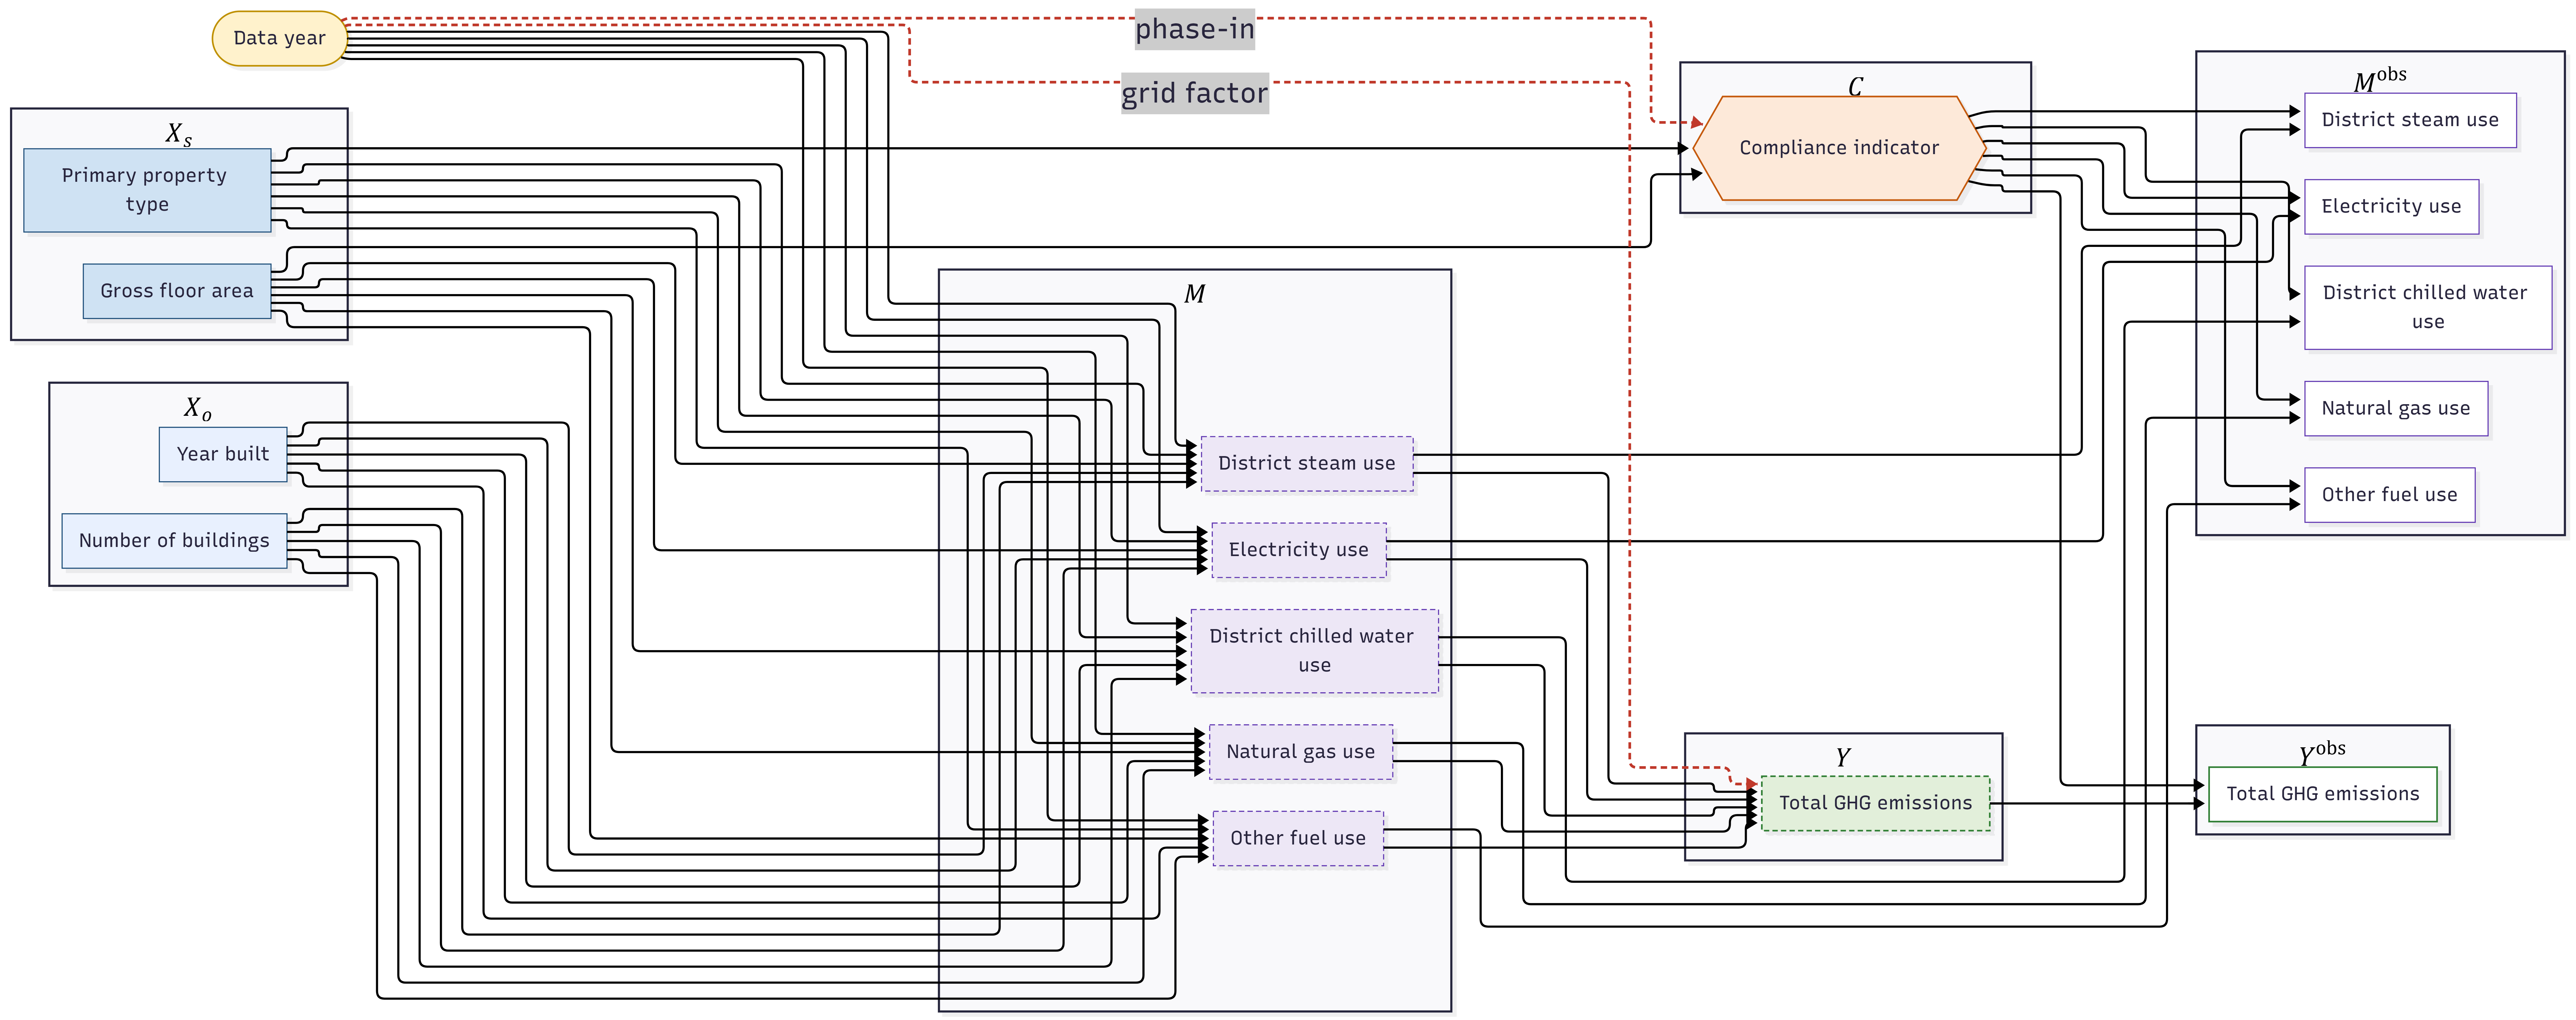
\includegraphics[width=0.98\linewidth]{figures/figure4_8.png}
\caption*{\textbf{Figure 4.8. Tested DAG for the Chicago data (Stage 3 output).} The candidate DAG of Figure 4.7 with the Stage-3 correction: the data year is lifted out of $X_o$ into a standalone period index and gains two edges (highlighted), one to the outcome $Y$ and one to the gate $C$ (see text). All other edges carry over from Figure 4.7; latent nodes are dashed-bordered. Author's construction.}
\end{figure}

All three predictions survive contact with documents that took no part in drawing the graph, and the two regressions add quantitative corroboration where the data can speak. The graph that results is a tested object rather than an asserted one (Figure 4.8): its selection edge is the ordinance's eligibility rule, its mediator/outcome split is the reporting schema's input/output distinction, and its $\mathrm{pa}(Y) = M$ claim is the EPA accounting identity, recovered from the data to $R^2 = 0.9999$. That is the warrant Sections 5 to 7 draw on when they run the full Pearlian analysis on the tested structure.


\FloatBarrier
\section{Causal Estimation}

A data-generating process that has survived Stage 3 licenses the full estimation pipeline, conditional on the ignorability assumption that Section 3.4 identifies. This section carries out the intervention rung of Pearl's ladder of causation on the Chicago data.

\subsection{The Experimental Question and the Two Analysts}

To demonstrate causal knowledge's contribution to the analytical process, we consider a theoretical situation: two analysts face the same dataset, the same research question, and the same methods, differing only in whether they are aware of the tested DGP. Both pursue the same objective, a model of emissions valid for the entire building stock, and any difference in their analyses is then attributable to causal knowledge alone.

Awareness of the tested DGP does not alter the causal analyst's objective; it alters the interpretation of the data at hand. The sample represents $P(Y \mid X, C = 1)$; the analyst recognises this as a biased view of the population $P(Y \mid X)$. The bias is corrected by reweighting the sample toward the population, the back-door adjustment the gate requires (Section 3.4). The tested DGP also determines the predictor set: the upstream causes alone, $\mathbf{X}_s$, $X_o$, and the period index. Mediators and derived fields are withheld as downstream of those causes. Cross-validation is grouped by building, so that no building appears in both the training and test folds. The resulting model targets the population relationship $P(Y \mid X)$, corrected for the selection the gate induces.

Unaware of the tested DGP, the causally-blind analyst pursues the same objective but interprets the same data differently. The conditional $P(Y \mid X, C = 1)$ is taken to be the population relationship $P(Y \mid X)$, and the reporting subset is treated as representative of the full stock. With no discrepancy perceived, no correction is applied; the task reduces to predicting the recorded emissions as accurately as possible. Every available field is retained as a predictor, the mediators and derived fields among them. The sample is left unweighted, and cross-validation is performed without grouping, ignoring the panel structure. The resulting model fits the reporting buildings well, but is biased as an estimate of the city-wide relationship.

The next section makes the comparison precise, crossing each analyst's pipeline with a range of functional forms.

\subsection{The Factorial Design}

The comparison is made precise by crossing the two pipelines with three functional forms, producing a 2$\times$3 factorial in which each contribution can be isolated independently. The three forms span the two-cultures question (\cit{breiman2001}{Breiman, 2001}): OLS as the classical structural baseline, XGBoost as the algorithmic culture, and a hierarchical Bayesian model as the structural culture with calibrated uncertainty.

{
\footnotesize
\setlength{\tabcolsep}{5pt}
\renewcommand{\arraystretch}{1.15}
\begin{longtable}{lrr}
\toprule
 & Causally blind & Causal pipeline \\
\midrule
\endfirsthead
\toprule
 & Causally blind & Causal pipeline \\
\midrule
\endhead
\bottomrule
\endlastfoot
\textbf{Linear} & M1: CB OLS & M4: IPW OLS \\
\textbf{Flexible (algorithmic)} & M2: CB XGBoost & M5: IPW XGBoost \\
\textbf{Flexible (structural)} & M3: CB Hierarchical Bayes & M6: IPW Hierarchical Bayes \\
\end{longtable}
}

The factorial structure separates the two contributions by holding one fixed while varying the other. Reading down a column holds the functional form fixed and varies only the pipeline, so any performance difference is attributable to the causal correction alone. Reading across a row holds the pipeline fixed and varies only the functional form. The comparison of primary interest is M5 against M6: both target the same population quantity from the same upstream features, and agreement between them on MdAPE is evidence that the tested DGP is sufficient to identify the population relationship (Section 3.4).

Four design choices separate the two pipelines, each determined by the tested DGP rather than by convention.

\begin{enumerate}
  \item \textbf{Feature set.} The causal pipeline uses the upstream causes only: $\mathbf{X}_s$, $X_o$, and the period index. The causally-blind pipeline retains every available field, including the mediators and derived performance fields.
  \item \textbf{Row subset.} The causal pipeline trains on compliant records only. The causally-blind pipeline trains on all records with an observed target, a slightly larger sample that nonetheless describes only the reporting buildings. This asymmetry is deliberate: each pipeline receives the data exactly as its analyst would actually prepare it.
  \item \textbf{Selection correction.} The causal pipeline reweights observations by the inverse propensity of compliance. The causally-blind pipeline applies no reweighting.
  \item \textbf{Cross-validation protocol.} The causal pipeline groups all observations of a building into the same fold (GroupKFold on building identity), reflecting the panel structure. The causally-blind pipeline uses ordinary $k$-fold, treating each row as independent.
\end{enumerate}

\subsection{The Propensity Model}

Selection is corrected by estimating the probability of compliance as a function of the upstream features. A logistic regression of the compliance indicator $C$ on $\mathbf{X}_s$, $X_o$, and the period index yields propensity scores $\hat{e}(X) = P(C = 1 \mid X)$. Property type is one-hot encoded because the ordinance defines the reporting obligation categorically by property class, with no ordinal structure across the 63 types the dataset records (Sections 4.1, 4.4). The period index is included because the tested DGP marks it as a parent of the compliance gate (Figure 4.8); the ordinance was phased in over successive years, so the probability of compliance depends on timing as well as building characteristics.

The model is fitted on all 28,329 records, compliant and non-compliant alike, since the gate can be learned only from both sides. This requires the upstream features to be complete, and in the raw file they are not: floor area is null in 7.8\% of records, property type in 15.0\%, year built in 17.8\%, and building count in 15.7\% (Section 4.1). A single shared preprocessing step, applied before either pipeline runs, fills the numeric upstream features with their global medians computed over all 28,329 records prior to any filtering, and assigns missing property types an explicit Unknown category that is one-hot encoded like any other class. This is the preprocessing step that the class definition of Section 2.1 anticipates for upstream fields with real missingness; it is identical for the causal and causally-blind pipelines, so no difference between their results can originate in it. Inputs are standardised before the logistic fit.

The resulting weights are moderate, indicating adequate overlap on the observed upstream characteristics. Raw inverse probability weights $w_i = 1 / \hat{e}(X_i)$ are trimmed at the 99th percentile and normalised to mean one (\cit{colehernan2008}{Cole \& Hernán, 2008}); the largest resulting weight is 1.32, so even the most underrepresented compliant building exerts only 32\% more influence than average. The propensity model classifies compliance at 95.1\% accuracy on the full dataset. The correction addresses selection on observed covariates only; selection on unobserved factors such as building management quality or retrofit investment is not corrected and is carried as a limitation.

The back-door correction is applied in both model families through mechanisms suited to each. In the OLS and XGBoost models, the weights enter as observation weights in the fitting procedure. In the hierarchical Bayesian models, they are injected via a likelihood potential,

\[
\log p^*(\theta \mid \text{data}) = \log p(\theta \mid \text{data}) + \sum_i (w_i - 1) \cdot \log p(y_i \mid \mu_i, \sigma),
\]

which up-weights the log-likelihood contribution of underrepresented buildings in proportion to their normalised weight. This is the back-door adjustment of Section 3.4, applied at the level of the posterior (\cit{pearl2009}{Pearl, 2009, Ch. 3}).

\subsection{Model Specifications}

\textbf{OLS (M1 and M4).} Both models assume a linear relationship between the feature vector and the log-transformed outcome. For observation $i$, the model is:

\[
y_i \sim \text{Normal}(\mu_i,\; \sigma), \qquad \mu_i = \mathbf{x}_i^\top \boldsymbol{\beta}
\]

where $y_i = \log_{1+}(\text{GHG}_i)$, $\mathbf{x}_i$ is the feature vector including an intercept, and $\boldsymbol{\beta}$ is the coefficient vector. Minimising the residual sum of squares yields the closed-form OLS estimator:

\[
\hat{\boldsymbol{\beta}} = (\mathbf{X}^\top \mathbf{X})^{-1} \mathbf{X}^\top \mathbf{y}
\]

where $\mathbf{X}$ is the $n \times p$ design matrix and $\mathbf{y}$ is the $n$-vector of log-transformed outcomes. No hyperparameters are tuned.

M1 and M4 differ in feature set, row subset, and whether IPW reweighting is applied. M1 trains on the full causally-blind feature set ($N = 21{,}714$ rows) with no reweighting; string and boolean columns (property type, ZIP code, community area, reporting status, exempt flag) are one-hot encoded. M4 trains on upstream features only ($N = 21{,}406$ compliant rows), with property type one-hot encoded, and replaces the OLS estimator with its IPW-weighted counterpart:

\[
\hat{\boldsymbol{\beta}}_{\text{WLS}} = (\mathbf{X}^\top \mathbf{W} \mathbf{X})^{-1} \mathbf{X}^\top \mathbf{W} \mathbf{y}
\]

where $\mathbf{W} = \mathrm{diag}(w_1, \ldots, w_n)$ and $w_i$ is the normalised IPW weight for observation $i$ derived from the propensity model (Section 5.3).

\textbf{XGBoost (M2 and M5).} Both XGBoost models approximate the conditional expectation $\mathbb{E}[\log_{1+}(\text{GHG}) \mid \mathbf{x}]$ as an additive ensemble of $T$ regression trees (Chen \& Guestrin, 2016), a flexible nonparametric form that imposes no assumed functional relationship between GHG emissions and the input features:

\[
\hat{y}_i = \sum_{t=1}^{T} f_t(\mathbf{x}_i), \quad f_t \in \mathcal{F}
\]

where $\mathcal{F}$ is the space of regression trees with leaf weight vectors $\mathbf{w}_t$. At each boosting step, a new tree is fitted to the negative gradient of a squared-error loss in $\log_{1+}$ space. Complexity is penalised via

\[
\Omega(f_t) = \gamma L_t + \tfrac{1}{2}\lambda \|\mathbf{w}_t\|^2 + \alpha \|\mathbf{w}_t\|_1
\]

where $L_t$ is the number of leaves, $\gamma$ is the minimum loss reduction required to admit a split, $\lambda$ is L2 regularisation on leaf weights, and $\alpha$ is L1 regularisation. Additional capacity is controlled by the maximum tree depth, subsampling ratio (fraction of training observations drawn per tree), column-sampling ratios at the tree and node levels, and the minimum child weight (minimum total instance weight in a child node).

Both models are tuned via nested cross-validation, which keeps the hyperparameter search separate from the generalisation estimate so that the reported CV performance reflects a model tuned on the training data alone. The outer loop provides five independent evaluation folds; within each, an Optuna Tree-structured Parzen Estimator (TPE; Akiba et al., 2019) runs 60 trials on a three-fold inner loop, searching jointly over all capacity and regularisation hyperparameters listed above. The inner loop uses MdAPE as the Optuna objective, so hyperparameter selection directly optimises the primary evaluation metric; within each trial, XGBoost early stopping uses RMSE with a 30-round patience. The winning configuration is applied to the full outer-fold training set with $n_{\text{estimators}} = 2{,}000$ and a 50-round early-stopping patience; $n_{\text{jobs}} = 1$ ensures deterministic floating-point accumulation. The deployment model refits on all available training data under the hyperparameter configuration from the median inner tuning run. Categorical columns are label-encoded and boolean columns are coerced to integer; numeric columns are filled with their within-fold median.

M2 and M5 are architecturally identical but differ in the four pipeline respects established in Section 5.2. M2 trains on the full causally-blind feature set ($N = 21{,}714$ rows) under \code{KFold} with no IPW correction. M5 trains on upstream features only ($N = 21{,}406$ compliant rows) under \code{GroupKFold} on building identity, and IPW enters as sample weights passed to the XGBoost \code{fit} call. The \code{GroupKFold} structure is maintained in both the inner tuning loop and the outer evaluation folds, so that no building appears in both training and test sets at any stage of the M5 pipeline.

\textbf{M3, Causally-Blind Hierarchical Bayes.} M3 is a hierarchical Normal regression in $\log_{1+}$(GHG) space over upstream features and five fuel-type mediators, trained on the full causally-blind row set ($N = 21{,}714$) with no IPW correction. The full generative model is:

\[
\begin{aligned}
y_i &\sim \text{Normal}(\mu_i,\; \sigma) \\
\mu_i &= \alpha_{j[i]} + \beta_A \tilde{a}_i + \beta_B \tilde{b}_i + \beta_T \tilde{t}_i + \beta_Y \tilde{y}_i \\
      &\phantom{{}={}}\quad + \beta_E \tilde{e}_i + \beta_G \tilde{g}_i + \beta_S \tilde{s}_i + \beta_W \tilde{w}_i + \beta_O \tilde{o}_i \\
\alpha_j &= \bar{\alpha} + \delta_j \sigma_\alpha \\
\delta_j &\sim \text{Normal}(0,\; 1), \quad j = 1, \ldots, 63 \\
\bar{\alpha} &\sim \text{Normal}(7.0,\; 1.0) \\
\sigma_\alpha &\sim \text{HalfNormal}(1.0) \\
\beta_k &\sim \text{Normal}(0,\; 2.5), \quad k \in \{A, B, T, Y\} \\
\beta_f &\sim \text{Normal}(0,\; 2.0), \quad f \in \{E, G, S, W, O\} \\
\sigma &\sim \text{HalfNormal}(0.5)
\end{aligned}
\]

where $\tilde{a}_i$ and $\tilde{b}_i$ are log floor area and log building count centred at their training-fold means; $\tilde{t}_i$, $\tilde{y}_i$, $\tilde{e}_i$, $\tilde{g}_i$, $\tilde{s}_i$, $\tilde{w}_i$, $\tilde{o}_i$ are data year, year built, electricity, natural gas, district steam, district chilled water, and other fuel use, each standardised to zero mean and unit variance within the training fold. The global intercept prior $\text{Normal}(7.0, 1.0)$ is centred at $\exp(7) \approx 1{,}097$ metric tons CO$_2$e, close to the observed stock median, placing a weakly informative anchor on the unconditional GHG level. The upstream slope priors $\text{Normal}(0, 2.5)$ are agnostic about log-scale elasticities, reflecting the blind analyst's absence of structural prior knowledge about how area, age, or building count relate to emissions. The mediator priors $\text{Normal}(0, 2.0)$ are wide enough to allow the fuel slopes to recover the EPA emission-factor magnitudes from the data without constraining their values, while remaining informative enough to exclude implausibly large slopes. The non-centred parameterisation $\alpha_j = \bar{\alpha} + \delta_j \sigma_\alpha$ is required for NUTS convergence under weakly identified hierarchical parameters. The derived metrics, spatial indices, and compliance metadata present in the causally-blind training set are excluded from the likelihood. M3's generative model assigns explicit slope parameters only to upstream features and fuel mediators; those additional columns are available in the training data but do not enter the likelihood. The hierarchy spans all 63 property types in the causally-blind dataset. Like M6, M3 is evaluated via PSIS-LOO rather than held-out folds.

\textbf{M6, Causal Hierarchical Bayes.} M6 is a hierarchical Normal regression in $\log_{1+}$(GHG) space, fitted to the compliant row set ($N = 21{,}406$) with IPW applied via a likelihood potential. The full generative model is:

\[
\begin{aligned}
y_i &\sim \text{Normal}(\mu_i,\; \sigma) \\
\mu_i &= \alpha_{j[i]} + \beta_A \tilde{a}_i + \beta_B \tilde{b}_i + \beta_T \tilde{t}_i + \beta_Y \tilde{y}_i \\
\alpha_j &= \bar{\alpha} + \delta_j \sigma_\alpha \\
\delta_j &\sim \text{Normal}(0,\; 1), \quad j = 1, \ldots, 55 \\
\bar{\alpha} &\sim \text{Normal}(7.0,\; 1.0) \\
\sigma_\alpha &\sim \text{HalfNormal}(1.0) \\
\beta_k &\sim \text{Normal}(0,\; 0.5), \quad k \in \{A, B, T, Y\} \\
\sigma &\sim \text{HalfNormal}(0.5)
\end{aligned}
\]

where $\tilde{a}_i$ and $\tilde{b}_i$ are log floor area and log building count centred at their training-fold means, and $\tilde{t}_i$ and $\tilde{y}_i$ are data year and year built standardised to zero mean and unit variance. The global intercept prior $\text{Normal}(7.0, 1.0)$ is centred at $\exp(7) \approx 1{,}097$ metric tons CO$_2$e, close to the observed compliant-stock median. The non-centred parameterisation is required for NUTS convergence under weakly identified hierarchical parameters, as in M3. The upstream slope priors $\text{Normal}(0, 0.5)$ encode the causal analyst's expectation of near-unit log-scale elasticities: Stage 3 estimated the log-floor-area elasticity at approximately 1.0, meaning doubling floor area roughly doubles GHG emissions. This prior places 95\% of mass within $[-1, 1]$, encoding the expectation without constraining the remaining upstream slopes rigidly. IPW is injected via a likelihood potential (Section 5.3); the hierarchy spans the 55 property types present in the compliant training set.

Both Bayesian models share the same priors on $\sigma_\alpha$ and $\sigma$. The prior $\text{HalfNormal}(1.0)$ on $\sigma_\alpha$ allows type-level intercepts to vary by approximately $\pm 1$ log unit around the global mean, equivalent to a factor of $e \approx 2.7$ between the most and least emissions-intensive property types; this is consistent with the heterogeneity observed across office, warehouse, and multifamily residential building classes. The prior $\text{HalfNormal}(0.5)$ on $\sigma$ is weakly informative: a residual standard deviation of 0.5 on the log scale corresponds to multiplicative prediction errors of $\exp(0.5) \approx 1.65$ in the original scale, placing a soft upper bound on unexplained variation while leaving the data to determine the actual residual magnitude.

Both models are sampled with four chains, 3,000 warmup steps, and 3,000 post-warmup draws, using a target acceptance rate of 0.95 and \code{jitter+adapt\_diag} initialisation. Convergence is assessed by $\hat{R} < 1.01$ and bulk effective sample size $> 400$ for all structural parameters (\cit{vehtarietal2021}{Vehtari et al., 2021}). Predictive performance is evaluated via Pareto-smoothed importance-sampling leave-one-out cross-validation (PSIS-LOO; \cit{vehtarietal2017}{Vehtari et al., 2017}).

\subsection{Evaluation Metrics and Ex-Ante Predictions}

Each model is evaluated on five metrics: $R^2(\log)$, MdAPE, median RMSE, 89\% predictive interval coverage, and ELPD. Models are fitted and evaluated in $\log_{1+}$(GHG) space; point metrics ($R^2(\log)$ and RMSE) are reported on this scale. Together the five metrics capture complementary aspects of model performance that no single metric covers simultaneously for a right-skewed outcome: point accuracy, scale-invariant error, interval calibration, and predictive density.

\begin{enumerate}
  \item \textbf{$R^2(\log)$} is the proportion of log-scale variance explained. Values near 1.0 are expected whenever a model has access to near-identity inputs; an unusually high $R^2(\log)$ in this design is a diagnostic signal rather than a performance achievement.
  \item \textbf{MdAPE} is the primary evaluation metric. The median absolute percentage error is scale-invariant and per-building: a value of 20\% means the median building's estimate deviates from its true value by roughly a fifth, a quantity a policy analyst can reason about directly. MdAPE is preferred over mean-based error metrics because GHG emissions are right-skewed; a small number of very large buildings dominate absolute-error averages, making them uninformative for the typical building. Building-level GHG emissions vary substantially even among buildings with similar physical characteristics, due to occupant behaviour, equipment age, and operational schedules, all sources of variation that upstream physical features cannot capture and that set a practical floor on prediction error.
  \item \textbf{Median RMSE} is reported in metric tons CO$_2$e on the original scale. For OLS and XGBoost (M1, M2, M4, M5), RMSE is computed on the held-out test fold at each of the five CV splits and the median is taken across folds. For the Bayesian models (M3 and M6), there are no KFold splits; RMSE is instead computed from PSIS-LOO leave-one-out predictive means against observed values. The two procedures are on different computational bases and Bayesian RMSE values should not be compared directly to frequentist fold-median values.
  \item \textbf{89\% predictive interval coverage} reports the fraction of held-out observations that fall inside the model's 89\% predictive band. Values above 89\% indicate conservatively wide intervals; values below indicate over-confident intervals.
  \item \textbf{ELPD} is the primary criterion for the Bayesian models (M3 and M6). PSIS-LOO ELPD is a sum of log predictive densities; higher values indicate better-calibrated predictive distributions, and differences larger than roughly four units are practically meaningful. Because ELPD accumulates over observations, raw values are not directly comparable between models fitted on different row subsets. For OLS and XGBoost, ELPD is estimated via a normal approximation applied to CV prediction errors, since these models do not produce posterior predictive distributions; for the Bayesian models, ELPD is computed exactly via PSIS-LOO from the full posterior. The two methods are directionally consistent but not strictly on the same computational basis.
\end{enumerate}

The four predictions below follow from the experimental structure and the tested DGP alone; none draws on the results that Section 5.6 reports, so their corroboration or refutation is informative about the DGP's implications rather than fitted to the outcomes after the fact.

\begin{enumerate}
  \item \textbf{Convergence.} On the corrected foundation, M5 (IPW XGBoost) and M6 (IPW Hierarchical Bayes) will agree on MdAPE to within roughly one percentage point. With the tested DGP specifying the causal structure, the structural and algorithmic estimators answer the same population-level question and have no quantity to disagree about.
  \item \textbf{The cost of correction.} Within every functional form, the causal pipeline will show higher apparent cross-validation error than its causally-blind counterpart. The blind advantage reflects selection and co-outcome leakage, not generalisation; its presence is expected and informative rather than a failure of the causal pipeline.
  \item \textbf{The accounting artefact.} The causally-blind XGBoost (M2) will attain unusually low cross-validation error by exploiting derived fields (site EUI, source EUI, national median EUI) that encode a near-identity with the GHG outcome. SHAP mediator attribution will confirm that this apparent accuracy reflects an accounting relationship rather than predictive skill over upstream inputs.
  \item \textbf{Deployment separation.} Applied to non-compliant buildings, the causal models will produce stable and well-defined estimates; the causally-blind models will produce unreliable estimates, because their derived-field predictors are unobserved for buildings that never reported.
\end{enumerate}

\subsection{Results and Diagnostics}

\subsubsection*{Experimental Results}

Table 5.1 below reports out-of-sample $R^2(\log)$, MdAPE, median RMSE, 89\% predictive interval coverage, and ELPD for all six models; Figure 5.1 plots the same results for visual comparison. The bottom panel of Table 5.1 reports the IPW effect as the difference between causal and causally-blind within each functional form; a positive value indicates the causal pipeline has higher apparent error. Results are discussed in the order of the four ex-ante predictions from Section 5.5.

\par\medskip\noindent
{\small\itshape \textbf{Table 5.1. Out-of-sample results, 2$\times$3 factorial experiment.} The bottom panel (IPW effect = causal minus causally-blind) shows that the causal pipeline records higher apparent CV error for OLS (+8.0 pp) and ML (+18.9 pp); this is expected, as the causally-blind advantage reflects circular feature leakage rather than genuine predictive skill. The convergence of M5 and M6 to within 0.4 pp is the central finding: XGBoost and Hierarchical Bayes agree because the tested DGP fixes the target quantity. The near-zero M3--M6 Bayesian gap and its deployment implications are examined in the diagnostics below. †Bayesian RMSE and ELPD use different computational bases from frequentist models; see Section 5.5 for details.\par}
\nopagebreak\medskip\nopagebreak
{
\footnotesize
\setlength{\tabcolsep}{5pt}
\renewcommand{\arraystretch}{1.15}
\begin{longtable}{lrrrrrr}
\toprule
Pipeline & Model & $R^2(\log)$ & MdAPE & Med. RMSE† & 89\% PI cov. & ELPD \\
\midrule
\endfirsthead
\toprule
Pipeline & Model & $R^2(\log)$ & MdAPE & Med. RMSE† & 89\% PI cov. & ELPD \\
\midrule
\endhead
\bottomrule
\endlastfoot
\textbf{Causally-blind} & M1 OLS & +0.756 & 31.5\% & 174,020 & 93.8\% & -17,075 \\
 & M2 XGBoost & +0.993 & 2.1\% & 1,185 & 96.7\% & +22,317 \\
 & M3 Hier. Bayes† & +0.848 & 20.9\% & 213 & 92.4\% & -11,935 \\
\textbf{Causal} & M4 OLS & +0.557 & 39.5\% & 129,691 & 93.1\% & -22,716 \\
 & M5 XGBoost & +0.835 & 21.0\% & 2,584 & 92.4\% & -12,491 \\
 & M6 Hier. Bayes† & +0.838 & 21.4\% & 218 & 92.8\% & -12,316 \\
\textbf{IPW effect} (causal - CB) & Frequentist & -0.199 & +8.0 pp & -44,328 & -0.7 pp & -5,641 \\
 & ML & -0.158 & +18.9 pp & +1,399 & -4.3 pp & -34,809 \\
 & Bayesian & -0.010 & +0.4 pp & +5 & +0.4 pp & -378 \\
\end{longtable}
}
\par\medskip

One feature of Table 5.1 needs comment before the predictions are assessed. The six-figure median RMSE values for the two OLS models (M1: 174,020; M4: 129,691 t CO$_2$e) reflect exponential back-transformation rather than a broken pipeline: all models are fitted in $\log_{1+}$ space, and an OLS log-scale error of a few units on one of the largest buildings becomes an original-scale residual of hundreds of thousands of tons, which a squared-error metric then amplifies. MdAPE is the primary metric for precisely this reason (Section 5.5), and the same extrapolation behaviour reappears as the heavy right tails of M1 and M4 in the deployment distributions (Figure 5.2).

\begin{figure}[tbp]
\centering
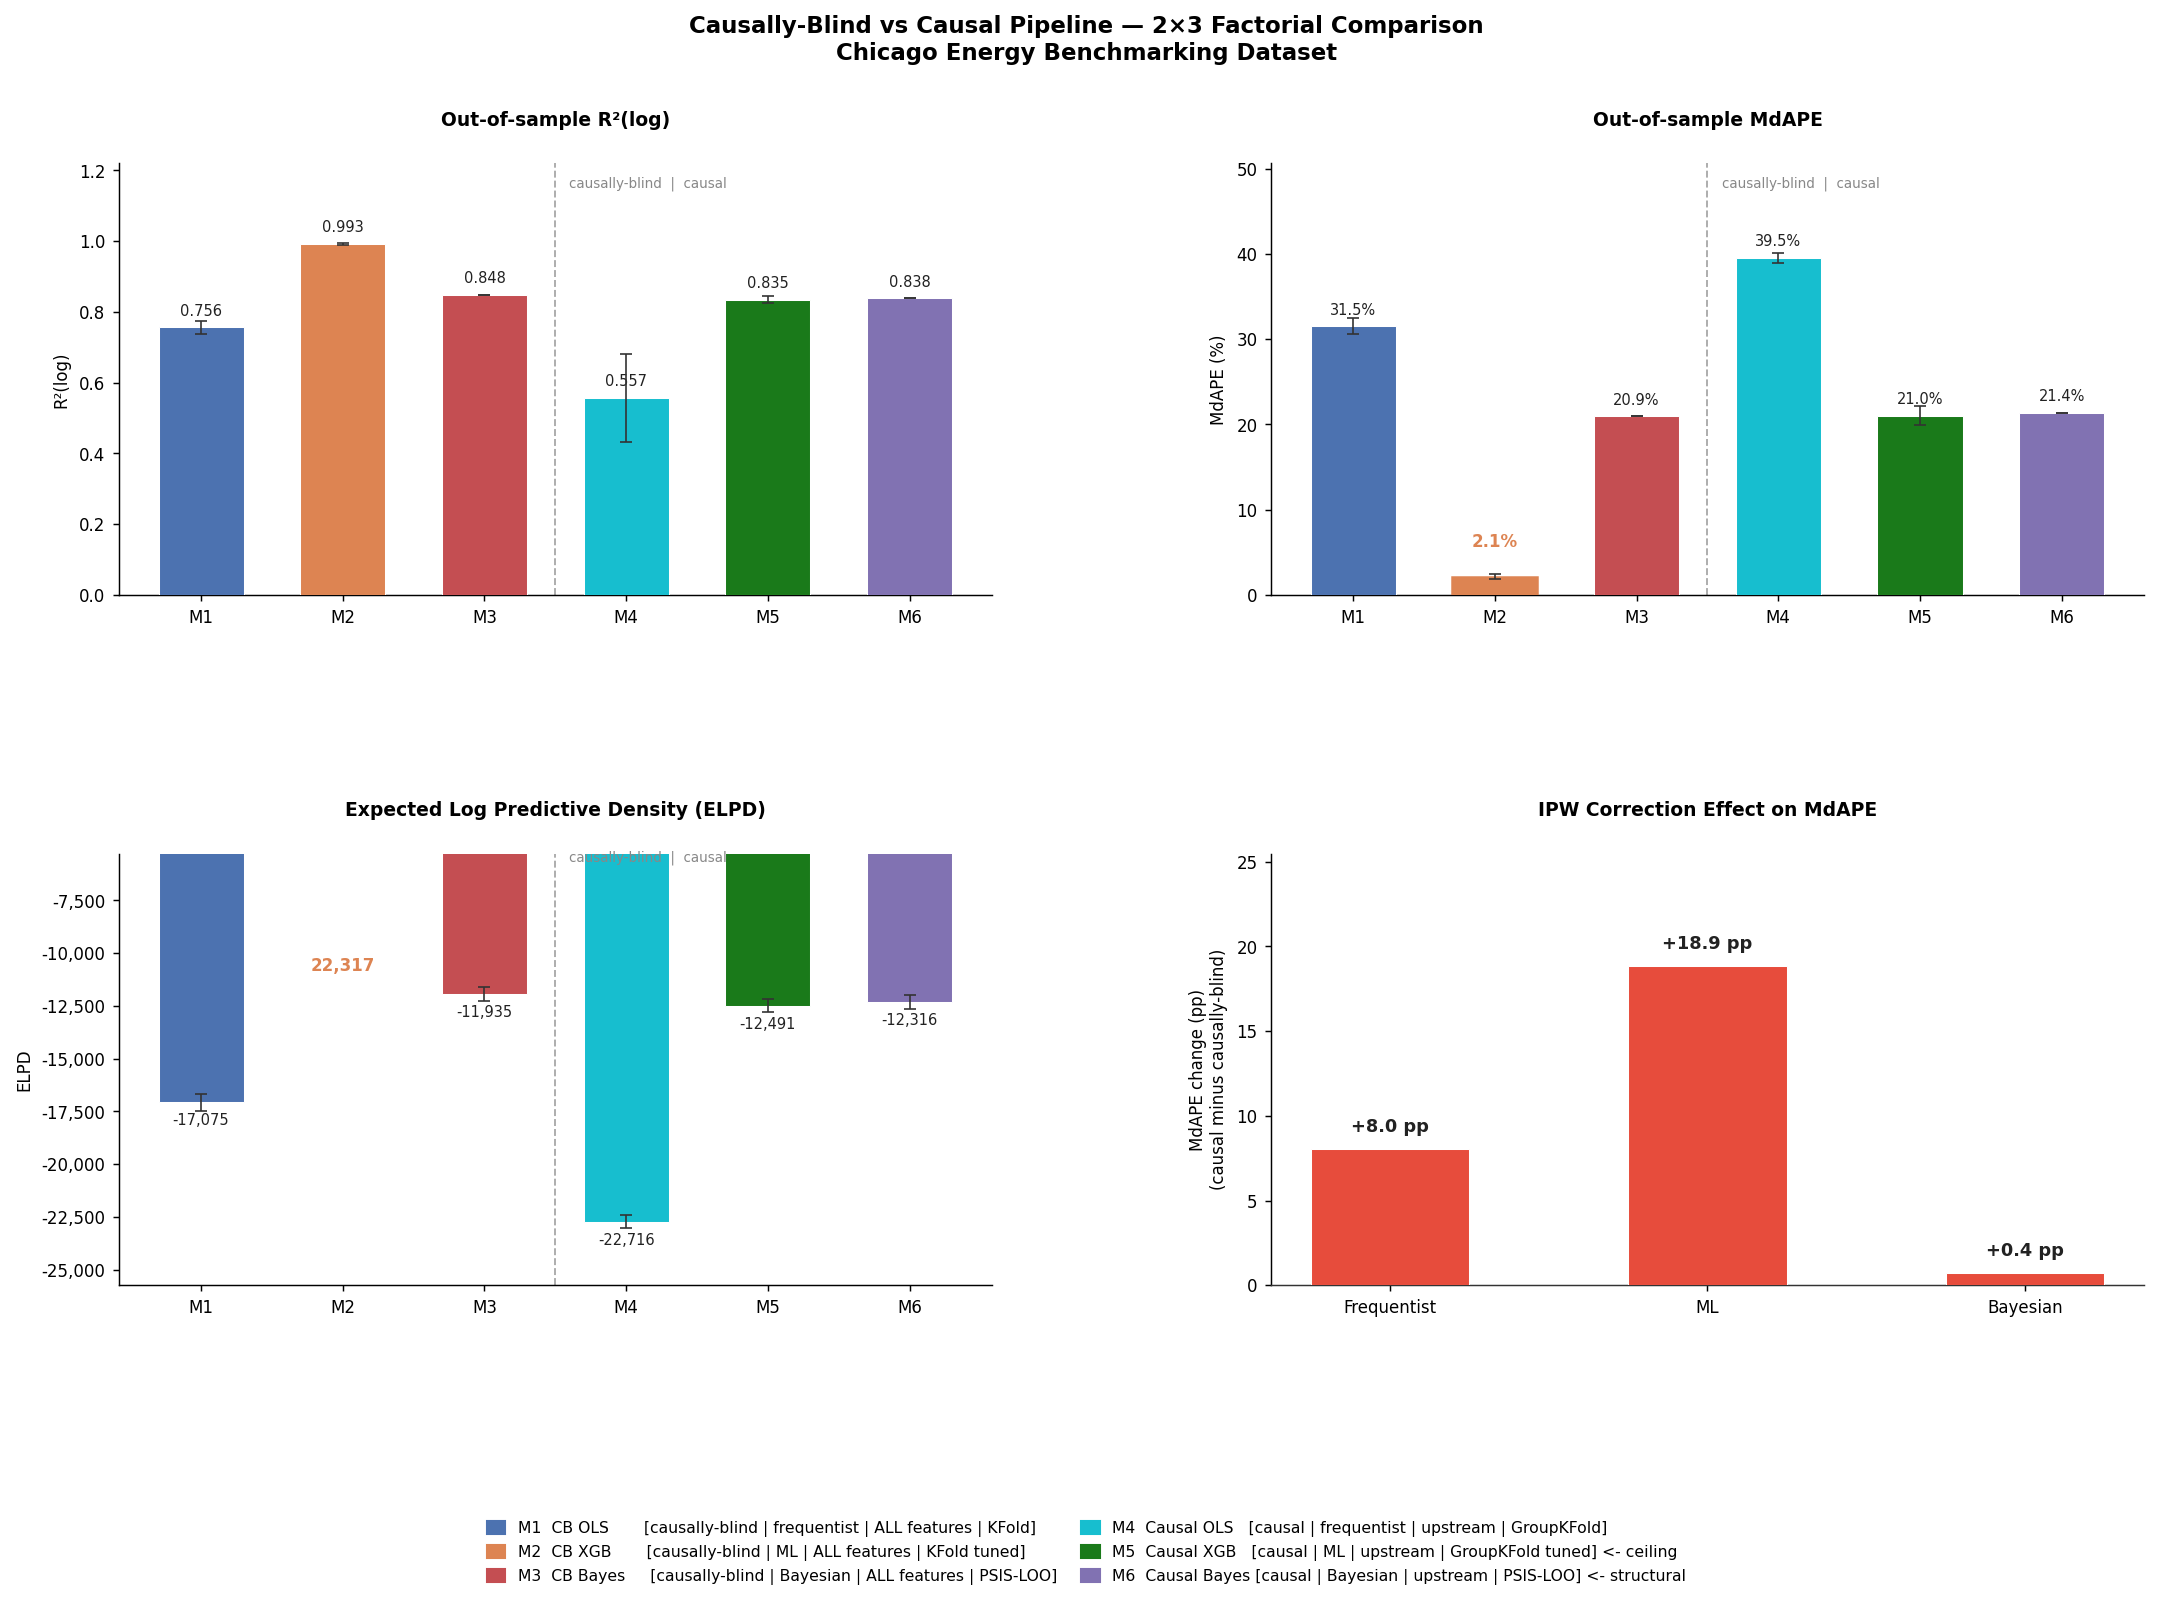
\includegraphics[width=0.95\linewidth]{figures/fig_comparison.png}
\caption*{\textbf{Figure 5.1. Causally-blind vs causal pipeline, 2$\times$3 factorial comparison.} M5 and M6 converge to within 0.4 percentage points on MdAPE; M2 (CB XGBoost) is the clear outlier at 2.1\%. The IPW correction cost is large for OLS (+8.0 pp) and ML (+18.9 pp) but negligible for Bayesian (+0.4 pp). Author's analysis of Chicago Energy Benchmarking data.}
\end{figure}

\textbf{Prediction 1: Convergence (corroborated).} M5 (IPW XGBoost) records MdAPE = 21.0\% and M6 (IPW Hierarchical Bayes) records MdAPE = 21.4\%, a gap of 0.4 percentage points well within the predicted threshold of one percentage point. The convergence holds across the building-size distribution: Figure 5.3 breaks MdAPE down by floor-area quintile, and M5 and M6 remain within 1.5 percentage points of each other across all five quintiles, from the smallest buildings (Q1: 22.5\% vs 22.4\%) to the largest (Q5: 18.3\% vs 18.3\%). The ELPD comparison (M6: $-12{,}316$ versus M5: $-12{,}491$, a difference of 175 units) is marginal and in M6's favour. Where the two estimators agree on prediction, the structural model is preferred: M6 additionally provides interpretable posterior coefficients and calibrated uncertainty intervals at no accuracy cost, and those parameters are the subject of Section 6. This convergence is the paper's central empirical finding: when the data-generating process is tested, structural and algorithmic models estimate the same causal quantity and produce equivalent predictions, resolving the two-cultures tension under the specific condition that the DGP is recoverable from institutional documentation.

MCMC diagnostics confirm reliable sampling for both Bayesian models. M3: $\hat{R}_{\max} = 1.004$, $\text{ESS}_{\min} = 548$, zero divergent transitions, and 5 observations with Pareto-$k > 0.7$ across 21,714 data points (indicating observations whose LOO influence is difficult to estimate reliably). M6: $\hat{R}_{\max} = 1.010$, $\text{ESS}_{\min} = 526$, zero divergent transitions, and 1 observation with Pareto-$k > 0.7$ across 21,406 data points. Both satisfy the $\hat{R} < 1.01$ and bulk $\text{ESS} > 400$ thresholds (\cit{vehtarietal2021}{Vehtari et al., 2021}). The marginally elevated $\hat{R}$ in M6 reflects the additional curvature introduced by the IPW potential in the log-posterior and does not indicate convergence failure.

\textbf{Prediction 2: The cost of correction (corroborated).} $\Delta\text{MdAPE} = \text{MdAPE}_{\text{causal}} - \text{MdAPE}_{\text{CB}}$ is positive in all three approach pairs: $+8.0$ pp for OLS (M4 vs M1), $+18.9$ pp for XGBoost (M5 vs M2), and $+0.4$ pp for Bayesian (M6 vs M3). The causal pipeline records higher apparent CV error in every row of the factorial, as predicted. An analyst reading Table 5.1 without causal domain knowledge would select M2 on CV metrics and deploy a causally invalid model.

\textbf{Prediction 3: The accounting artefact (corroborated).} M2 records $R^2 = 0.993$ and MdAPE = 2.1\% across five KFold splits, with fold-level $R^2$ ranging from 0.989 to 0.996. Figure 5.4 makes the artefact visible: M2's predicted vs actual scatter collapses onto the diagonal with near-zero residual variance, a pattern absent from every other model. Figure 5.3 confirms the artefact is not size-specific: M2's MdAPE is uniformly 1.8--2.8\% across all five floor-area quintiles, ruling out any explanation based on the dominance of a particular building class. The ELPD gap between M2 ($+22{,}317$) and M5 ($-12{,}491$) is 34,808 units, the largest pairwise difference in the factorial. Figure 5.5 traces M2's metrics to SHAP-quantified feature exploitation.

\textbf{Prediction 4: Deployment separation (corroborated).} Table 5.2 and Figure 5.2 report predicted GHG for the 5,510 non-compliant building-year records withheld from all model training. The causal models produce deployment medians of 854 (M4), 1,213 (M5), and 1,043 (M6) metric tons CO$_2$e, a 359-ton range attributable to estimator differences and consistent with the observed compliant-building median of $\approx$1,018 metric tons. Figure 5.2 shows the distribution of predicted GHG across all six models: M5 and M6 produce narrow, overlapping peaks centred near 1,000 metric tons, while M1 and M4 show heavy right tails from OLS extrapolation beyond the compliant training support; M1's mean (2,640 metric tons) is more than five times its median (486) as a result. The causally-blind models span 486 (M1) to 1,025 (M3) metric tons, a 539-ton spread among models nominally using the same data.

\par\medskip\noindent
{\small\itshape \textbf{Table 5.2. Deployment test: predicted GHG for 5,510 non-compliant building-year records.} Median is the primary statistic; means are inflated by OLS extrapolation outliers for M1 and M4. The observed compliant-building median is $\approx$1,018 metric tons CO$_2$e. Causal models cluster near this anchor; causally-blind models span a 539-ton range because each estimates a different effective quantity. Author's analysis of Chicago Energy Benchmarking data.\par}
\nopagebreak\medskip\nopagebreak
{
\footnotesize
\setlength{\tabcolsep}{5pt}
\renewcommand{\arraystretch}{1.15}
\begin{longtable}{lrrr}
\toprule
Model & Pipeline & Median (t CO$_2$e) & Mean (t CO$_2$e) \\
\midrule
\endfirsthead
\toprule
Model & Pipeline & Median (t CO$_2$e) & Mean (t CO$_2$e) \\
\midrule
\endhead
\bottomrule
\endlastfoot
M1 CB OLS & Causally-blind & 486 & 2,640 \\
M2 CB XGBoost & Causally-blind & 641 & 968 \\
M3 CB Hier. Bayes & Causally-blind & 1,025 & 1,184 \\
M4 Causal OLS & Causal & 854 & 3,865 \\
M5 Causal XGBoost & Causal & 1,213 & 1,701 \\
M6 Causal Hier. Bayes & Causal & 1,043 & 1,323 \\
\end{longtable}
}
\par\medskip

\begin{figure}[tbp]
\centering
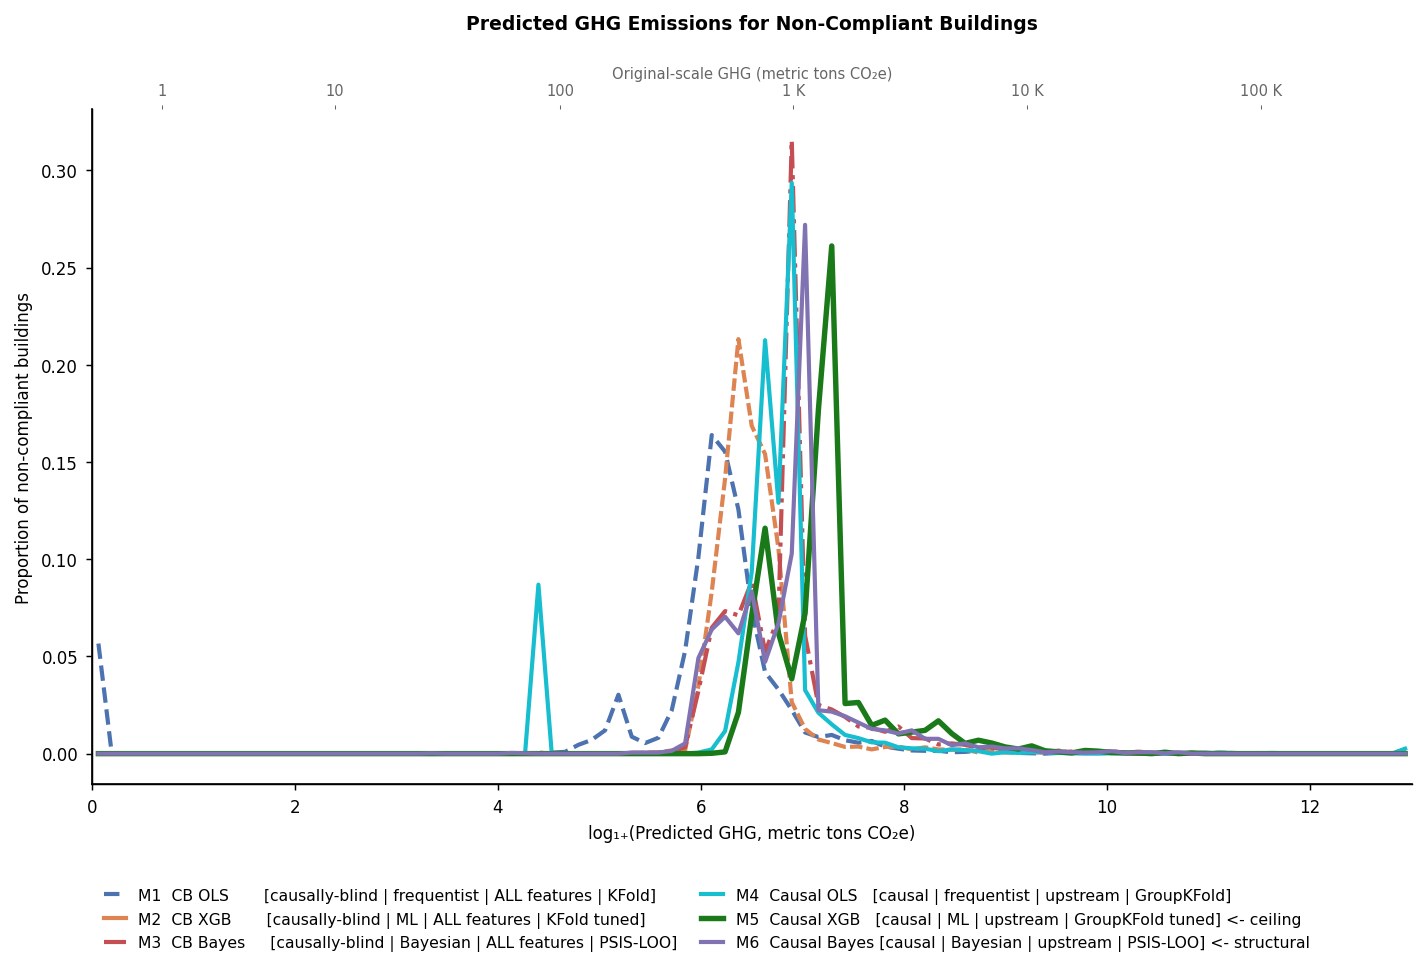
\includegraphics[width=0.95\linewidth]{figures/fig_deployment.png}
\caption*{\textbf{Figure 5.2. Predicted GHG emissions for 5,510 non-compliant building-year records.} Causal models (solid curves) converge on a narrow peak near 1,000 metric tons; causally-blind models (dashed curves) scatter across a 539-ton spread because each exploits the circular features differently and estimates a different effective quantity. M1's heavy right tail and M2's leftward shift are the signatures of OLS extrapolation and near-identity exploitation respectively. Author's analysis of Chicago Energy Benchmarking data.}
\end{figure}

\subsubsection*{Diagnostic Analysis}

The following diagnostics examine the mechanisms behind three results above: M2's near-perfect artefact, the near-zero Bayesian gap, and the divergence of causal and causally-blind models at deployment.

\begin{figure}[tbp]
\centering
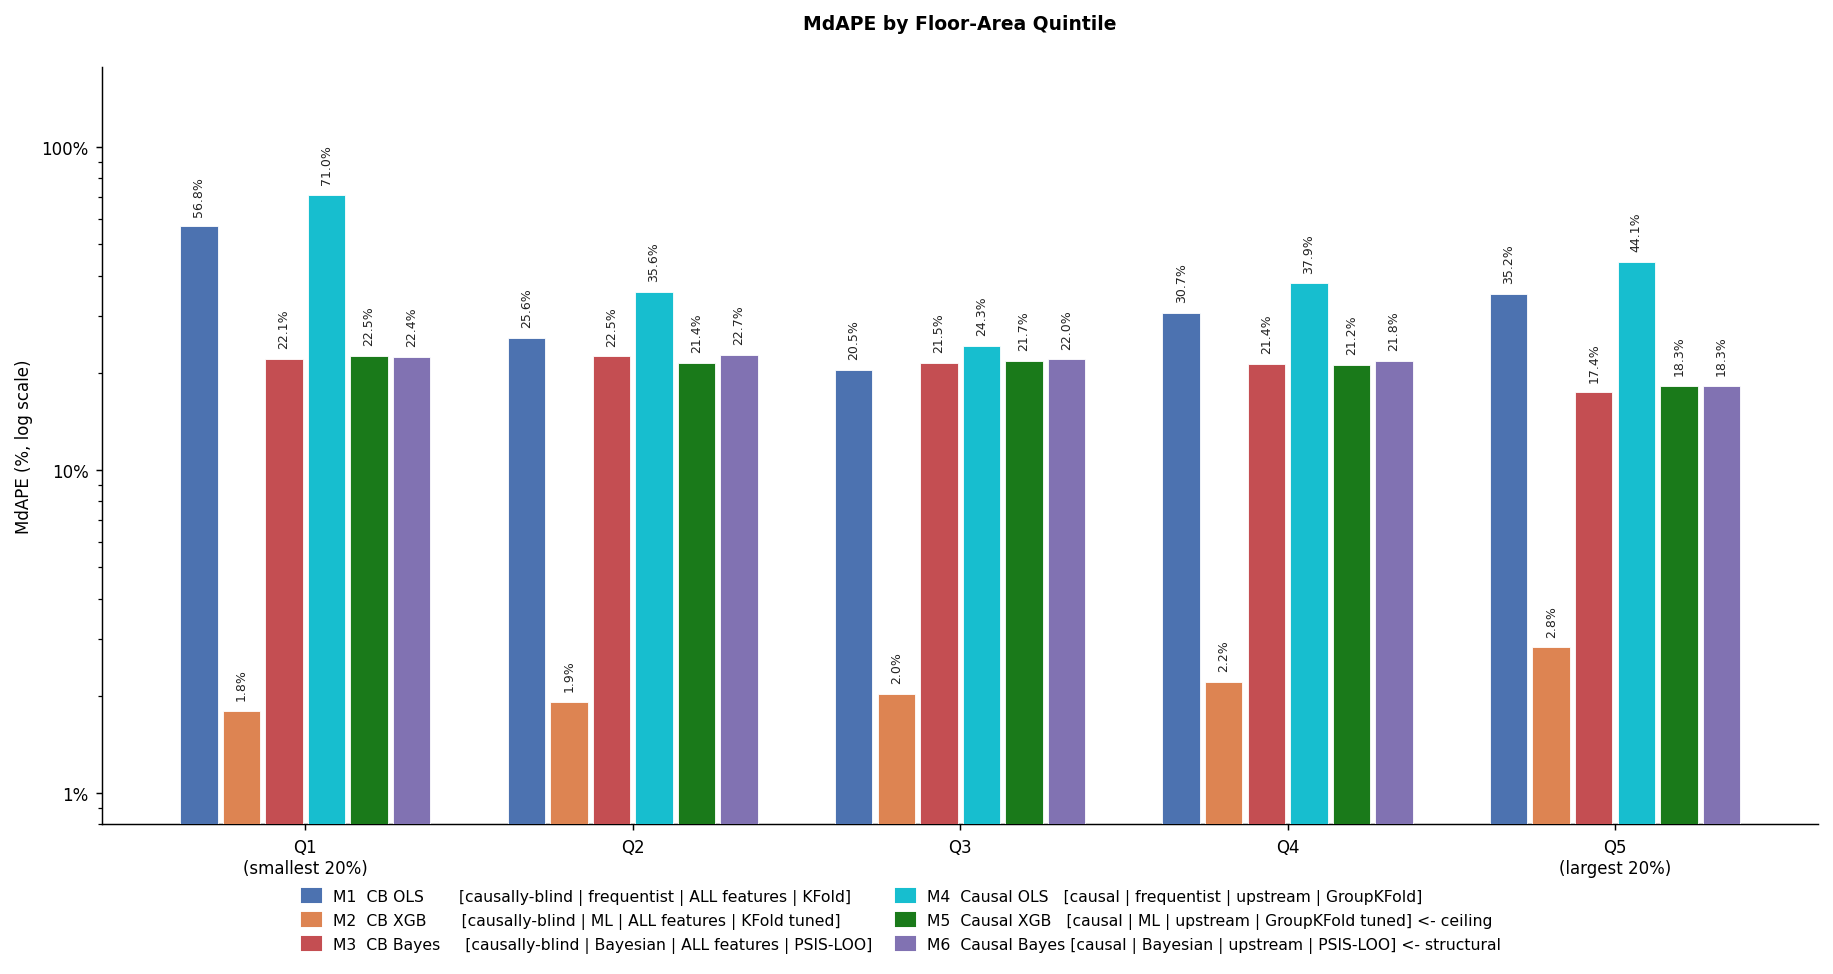
\includegraphics[width=0.95\linewidth]{figures/fig_quintile.png}
\caption*{\textbf{Figure 5.3. MdAPE by floor-area quintile, all six models.} Convergence of M5 and M6 holds at every floor-area quintile, ruling out a size-composition artefact behind the aggregate 0.4 pp gap. M2's MdAPE is uniformly near-zero across all quintiles, confirming the accounting artefact is structural rather than driven by any particular building class. Author's analysis of Chicago Energy Benchmarking data.}
\end{figure}

\begin{figure}[tbp]
\centering
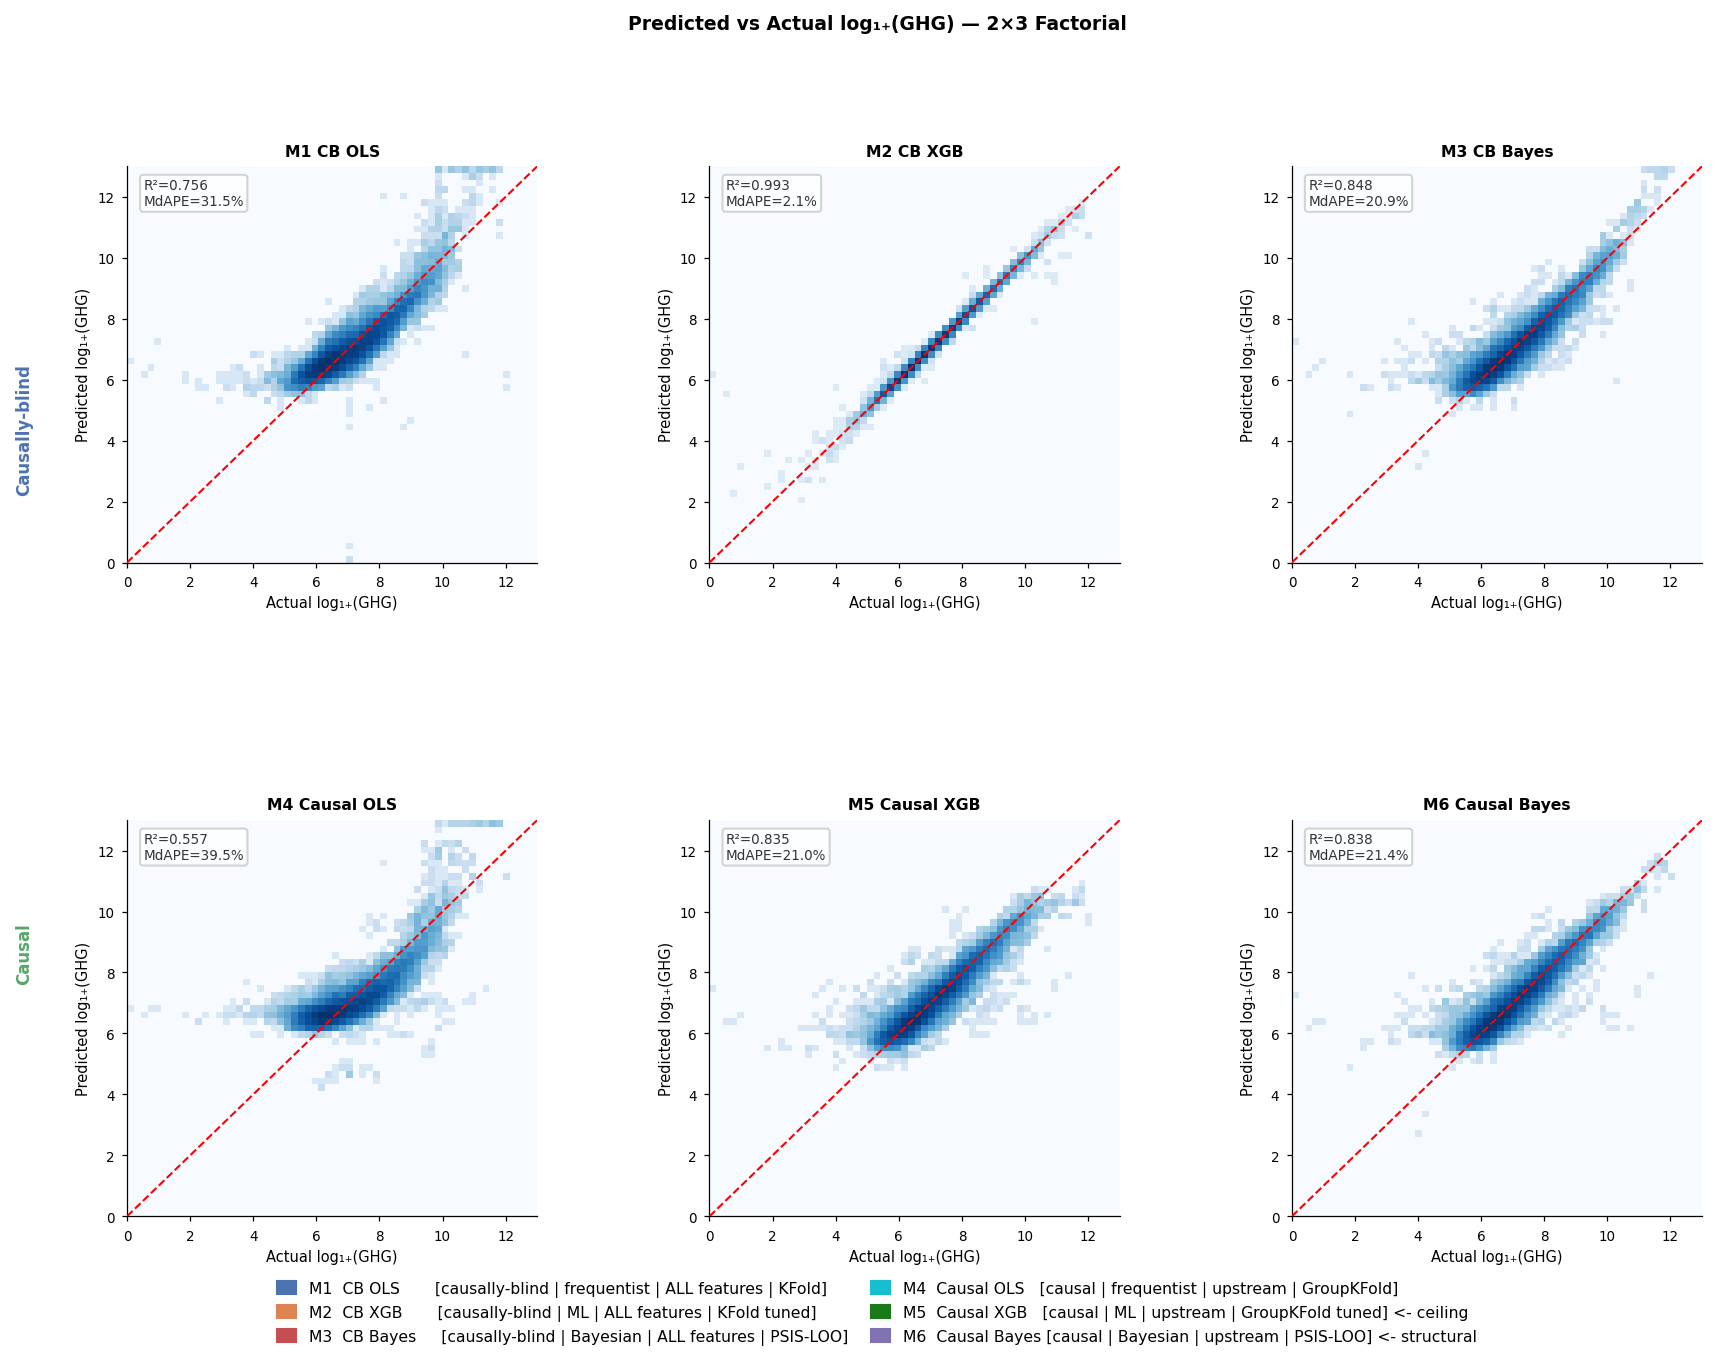
\includegraphics[width=0.95\linewidth]{figures/fig_pred_vs_actual.png}
\caption*{\textbf{Figure 5.4. Predicted vs actual $\log_{1+}$(GHG) for all six models, 2$\times$3 factorial.} M2's near-perfect diagonal collapse ($R^2 = 0.993$) is the accounting artefact made visible; the pattern is absent from every other model. M5 and M6 produce scatter-equivalent plots, confirming that functional form does not matter once the target quantity is fixed by the tested DGP. Author's analysis of Chicago Energy Benchmarking data.}
\end{figure}

\textbf{M2: accounting artefact mechanism.} SHAP group attribution (Figure 5.5a) quantifies what drives M2's metrics: energy mediators account for 57.2\% of M2's total predictive signal; derived/circular features (GHG intensity, site and source EUI, Energy Star score, Chicago Energy Rating) contribute a further 15.0\%; together 72.2\% of M2's signal comes from features that are either post-treatment or tautological. The dominant individual contributor is \code{electricity\_use\_kbtu} (42.3\%), through which XGBoost learns the direct EPA emission-factor mapping rather than any upstream causal structure. Only 26.1\% of M2's signal derives from upstream causal features, the only feature set causally valid at deployment and the sole basis on which M5 operates. Figures 5.5b and 5.5c make the mechanism concrete: even the highest-ranking upstream causal feature (log floor area, mean |SHAP| $\approx$0.23) is outweighed more than two-to-one by electricity alone, and the beeswarm confirms that the learned relationship is monotone and tight, the signature of a direct emission-factor mapping rather than a causal model of building characteristics.

\begin{figure}[tbp]
\centering
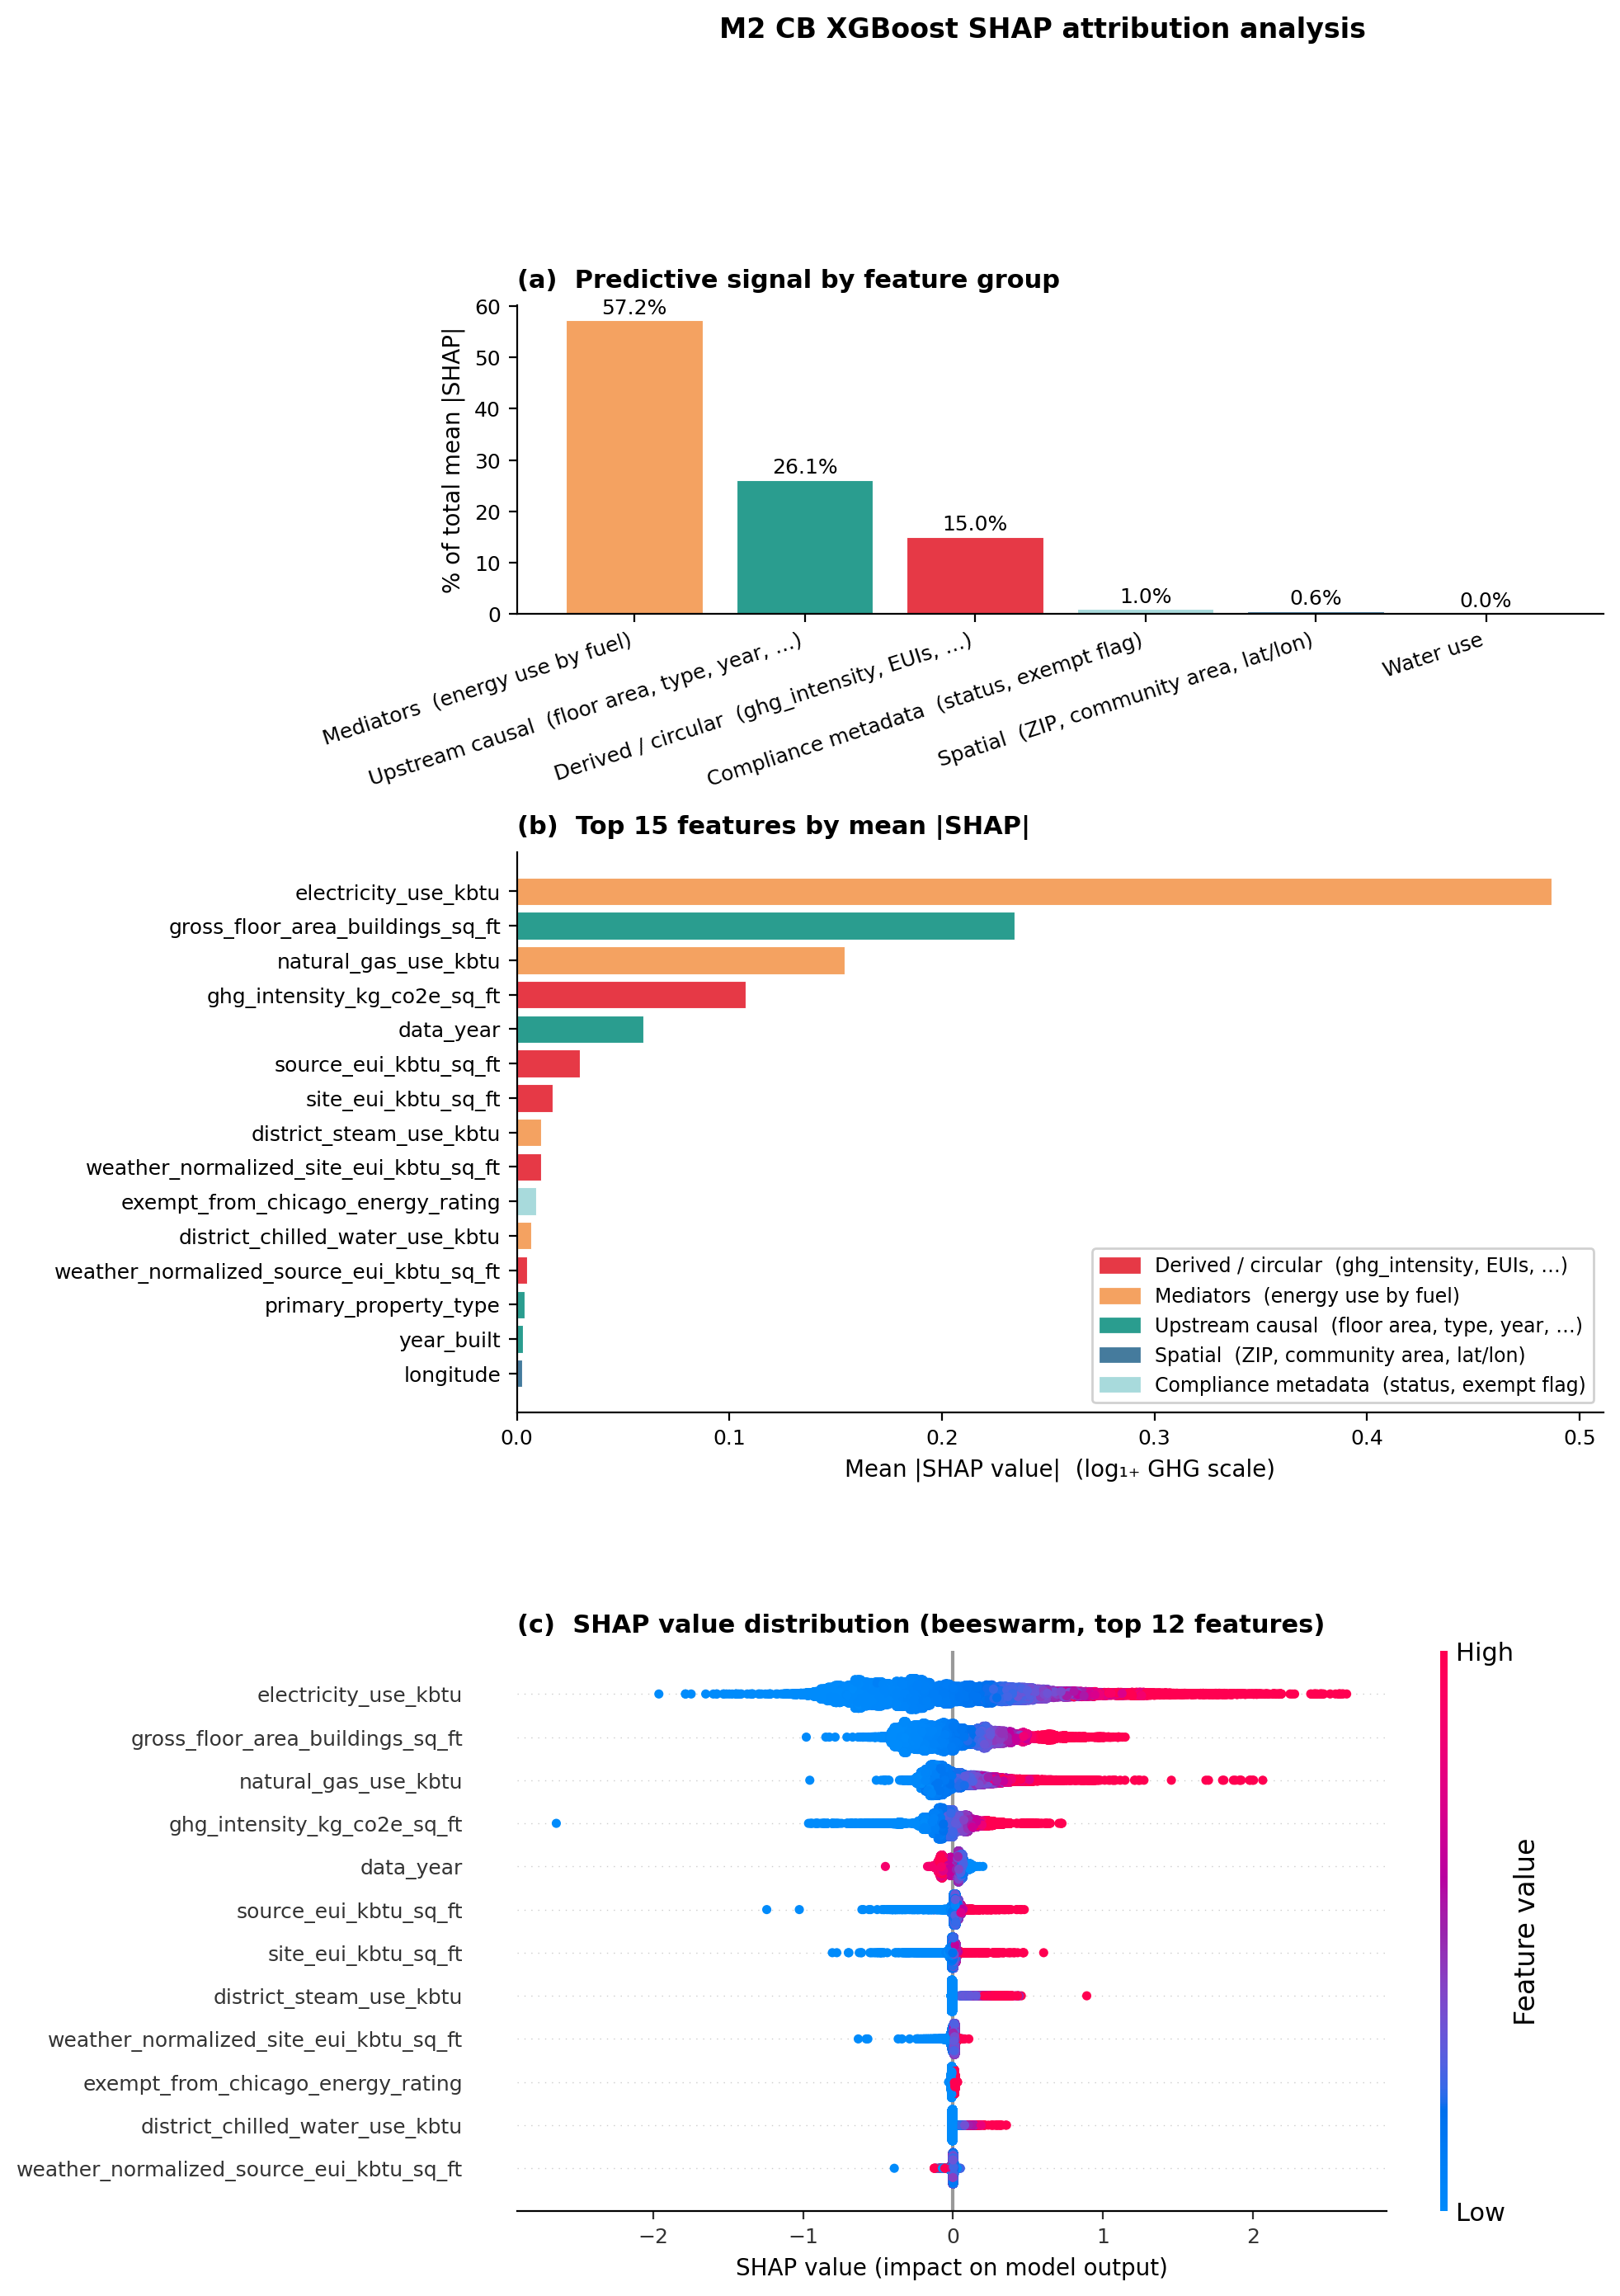
\includegraphics[width=0.8\linewidth]{figures/fig_shap_combined.png}
\caption*{\textbf{Figure 5.5. M2 CB XGBoost SHAP attribution analysis.} (a) Predictive signal by feature group: energy mediators account for 57.2\%; derived/circular features (GHG intensity, EUI variants, Energy Star score) contribute a further 15.0\%; together 72.2\% comes from features unavailable or causally invalid at deployment; upstream causal features contribute 26.1\%. (b) Top 15 features by mean |SHAP|: \code{electricity\_use\_kbtu} dominates at mean |SHAP| $\approx$0.49, more than double the next feature (\code{gross\_floor\_area\_buildings\_sq\_ft} at $\approx$0.23); apart from floor area, the top positions are held by mediators (orange) and derived/circular features (red), with the remaining upstream causal features (teal) in the lower half. (c) SHAP value distribution (beeswarm, top 12 features): \code{electricity\_use\_kbtu} and \code{natural\_gas\_use\_kbtu} show a strong monotone positive relationship, confirming XGBoost has learned the EPA emission-factor mapping directly; upstream causal features produce narrow, low-magnitude bands. Author's analysis of Chicago Energy Benchmarking data.}
\end{figure}

\textbf{M3 vs M6: the Bayesian gap.} The near-zero gap between M3 (20.9\%) and M6 (21.4\%) reflects a structural mis-match between M3's likelihood and the true EPA formula. The EPA GHG formula is additive in the original scale (GHG $= \sum_f \text{fuel}_f \times \varepsilon_f$); M3 models $\log_{1+}(\text{GHG})$ as linear in standardised fuel use, a specification that cannot represent an additive-in-levels sum: in log space, $\log\bigl(\sum_f \text{fuel}_f \times \varepsilon_f\bigr)$ is nonlinear in the individual fuels, so the log-linear coefficients cannot recover the emission-factor magnitudes. The posterior mediator slopes confirm the mis-match (Figure 5.6a): electricity use, the dominant driver of M2's 42.3\% SHAP signal, receives a posterior mean of only $+0.078$ on the standardised log scale, compared to log floor area at $+0.898$. District steam and all other fuel have 89\% posterior intervals that span zero. The log-linear specification assigns most explanatory power to log floor area (a proxy for scale that remains monotone with GHG even after log-transformation) and extracts only marginal signal from the mediators. M3 therefore cannot exploit its mediator access, and the 0.4 pp gap to M6 reflects near-equivalent predictive information rather than a genuine trade-off between mediator access and IPW correction. Figure 5.6b shows that M6's floor-area slope ($+0.979$) exceeds M3's ($+0.898$): without mediator slopes to distribute the scale signal, M6 assigns more explanatory weight to floor area.

\begin{figure}[tbp]
\centering
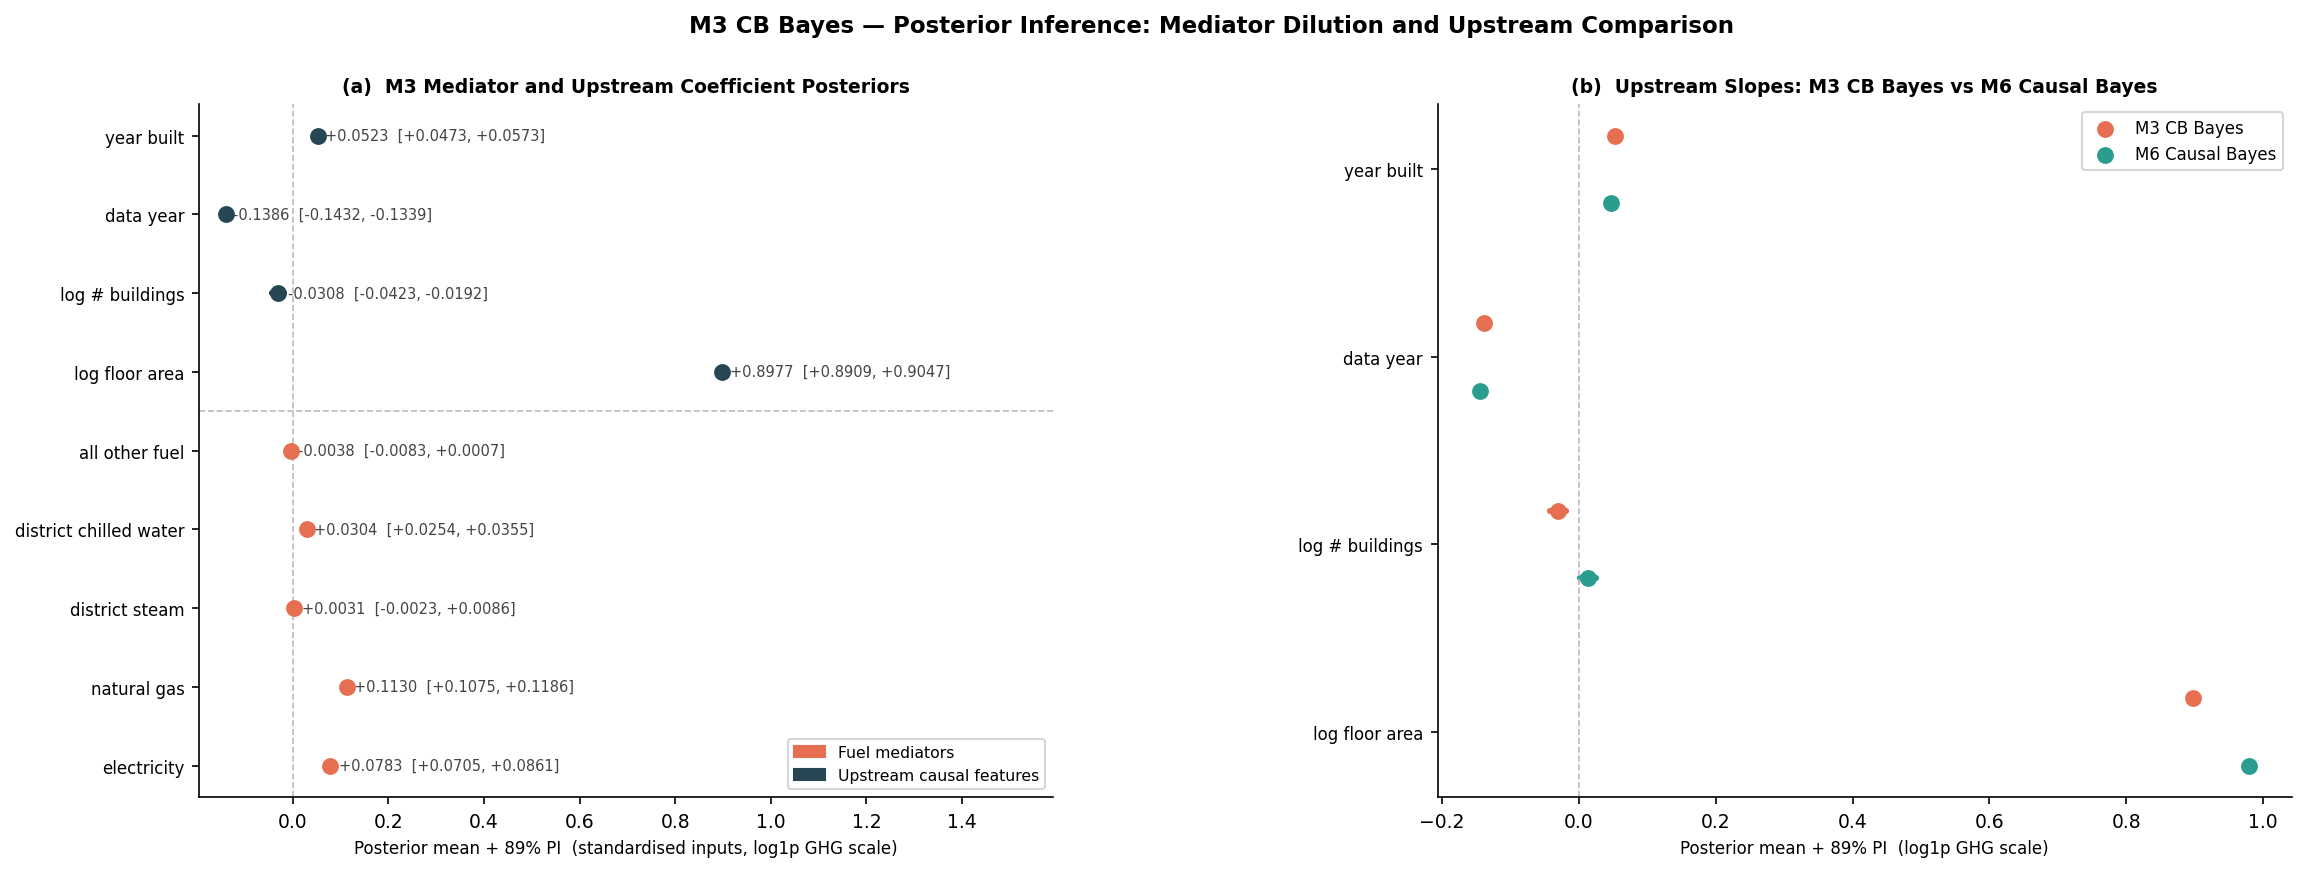
\includegraphics[width=0.95\linewidth]{figures/fig_m3_combined.png}
\caption*{\textbf{Figure 5.6. M3 CB Bayes posterior inference.} (a) Mediator and upstream coefficient posteriors (89\% PI): fuel mediator slopes (orange) are small relative to log floor area (teal, $+0.898$); electricity and natural gas are positive and precisely estimated but far below the floor-area coefficient; district steam and all other fuel have intervals spanning zero; the log-linear likelihood cannot recover the EPA emission-factor structure, leaving floor area to absorb the bulk of the explanatory signal. (b) Upstream slope comparison, M3 CB Bayes vs M6 Causal Bayes: M6's log floor-area slope ($+0.979$) exceeds M3's ($+0.898$) because M6 has no mediator slopes to share the scale signal with; the remaining upstream slopes are directionally consistent across models. Author's analysis of Chicago Energy Benchmarking data.}
\end{figure}

\textbf{Causally-blind deployment behaviour.} M2's deployment median (641 metric tons) is not near-zero: non-compliant buildings receive training-median imputation for all derived fields, so M2 predicts approximately $\hat{y}_i \approx \bar{g} \cdot a_i$ where $\bar{g}$ is the median GHG intensity and $a_i$ is floor area, the only feature that still varies across buildings. The prediction is numerically plausible but causally invalid; a practitioner without causal domain knowledge might accept it.

\subsubsection*{Discussion of Experimental Results}

Three limits bound these results. First, IPW corrects for selection on observed upstream characteristics; the unobserved component of selection (management practices, voluntary retrofits, tenant behaviour) remains uncorrected. The maximum normalised weight of 1.32 indicates moderate observed distortion, but the unobserved component is unbounded. The smallness of that maximum weight also bounds how much the correction does on this dataset: with weights this close to one, IPW shifts the causal estimates only modestly, so Chicago is a mild test of the selection machinery rather than a stringent one. The convergence and deployment results are therefore demonstrated under weak observed selection; a programme with a sharper gate or thinner overlap would exercise the correction far harder, and whether the same agreement survives there is exactly the cross-class replication Section 8 calls for. Second, the deployment test establishes ordinal plausibility relative to the compliant-building distribution; it does not provide ground-truth GHG for the 5,510 non-compliant building-year records, none of which have observed energy data. Third, M3's near-identical deployment prediction (1,025 metric tons versus M6's 1,043 metric tons) does not imply causal equivalence: M3's mediator slopes are too small to shift predictions materially from what upstream features alone produce, so the agreement reflects diluted coefficients rather than inherent Bayesian robustness to the compliance gate.

The 0.4 percentage-point gap between M5 and M6 means that functional form is not a source of uncertainty once the DGP is fixed: a flexible non-parametric estimator and a structural Bayesian model arrive at the same prediction when trained on the same causal foundation. That agreement is what the tested DGP predicted (Section 5.5), and within the limits stated above it corroborates the structure; it does not certify the structure beyond the observed support, where no ground truth exists. Subject to those limits, the posterior parameters of M6 are interpretable as estimates of causal quantities, and Section 6 examines them.


\FloatBarrier
\section{Structural Inference from the Focal Model}

Section 5 settled the predictive question: on the corrected causal foundation, the structural Bayesian model M6 matches the unconstrained ensemble M5 to within 0.4 percentage points of MdAPE. This section reports what that tie purchases. M5's output is a prediction; M6's output is a posterior distribution over the parameters of the population relationship $P(Y \mid X)$ that the pipeline targets, and those parameters carry physical and policy meaning unavailable from any point prediction. Four parameters carry the section's empirical claims, and they were declared as the parameters of interest before any robustness fits were run (Section 6.5): $\beta_A$, the floor-area elasticity; $\beta_T$, the data-year trend; $\sigma_\alpha$, the between-type heterogeneity; and $\sigma$, the residual scale. The remaining slopes $\beta_B$ and $\beta_Y$ are auxiliary controls. Because M6 regresses the outcome on the upstream features alone, its slopes estimate the reduced form of the world layer: the composite causal path from building characteristics through energy use into emissions. All results in this section are drawn from the same fitted posterior evaluated in the factorial experiment: the trace was saved at fit time (4 chains, 3,000 post-warmup draws each) and re-loaded for this analysis, so every number here is consistent with Table 5.1 by construction.

\subsection{Posterior Health and Calibration}

Inference is only as good as the sample that carries it, so the diagnostics come first. Across all parameters, $\hat{R}_{\max} = 1.0095$ and $\text{ESS}_{\min} = 526$, within the $\hat{R} < 1.01$ and bulk ESS $> 400$ thresholds (\cit{vehtarietal2021}{Vehtari et al., 2021}), with zero divergent transitions across 12,000 draws. The slowest-mixing parameters are the global hyperparameters $\bar{\alpha}$ and $\sigma$; the 55 property-type offsets mix far faster ($\text{ESS}_{\min} = 11{,}409$), which is the expected signature of the non-centred parameterisation. The type-level offsets $\delta_j$ are nearly decorrelated by construction, while the global scalars must integrate over all type-level uncertainty.

The predictive side is checked by Pareto-smoothed importance-sampling leave-one-out cross-validation (PSIS-LOO; \cit{vehtarietal2017}{Vehtari et al., 2017}). The ELPD of $-12{,}316$ (SE $317.4$) reproduces the experiment's reported value exactly, confirming the loaded trace is identical to the posterior evaluated in the factorial. The Pareto-$k$ diagnostic flags observations whose removal would substantially change the posterior and for which the LOO approximation is unreliable: 1 of 21,406 observations exceeds $k = 0.7$, and 7 exceed $k = 0.5$. The median $k$ of $-0.060$ indicates that the typical held-out observation is, if anything, more consistent with the model than the average one, the opposite of overfitting. Interval calibration was already quantified in Table 5.1: 92.8\% empirical coverage at the 89\% nominal level, slightly conservative. Figure 6.1 overlays 200 posterior predictive replications on the observed outcome distribution on both the log and original scales.

\begin{figure}[tbp]
\centering
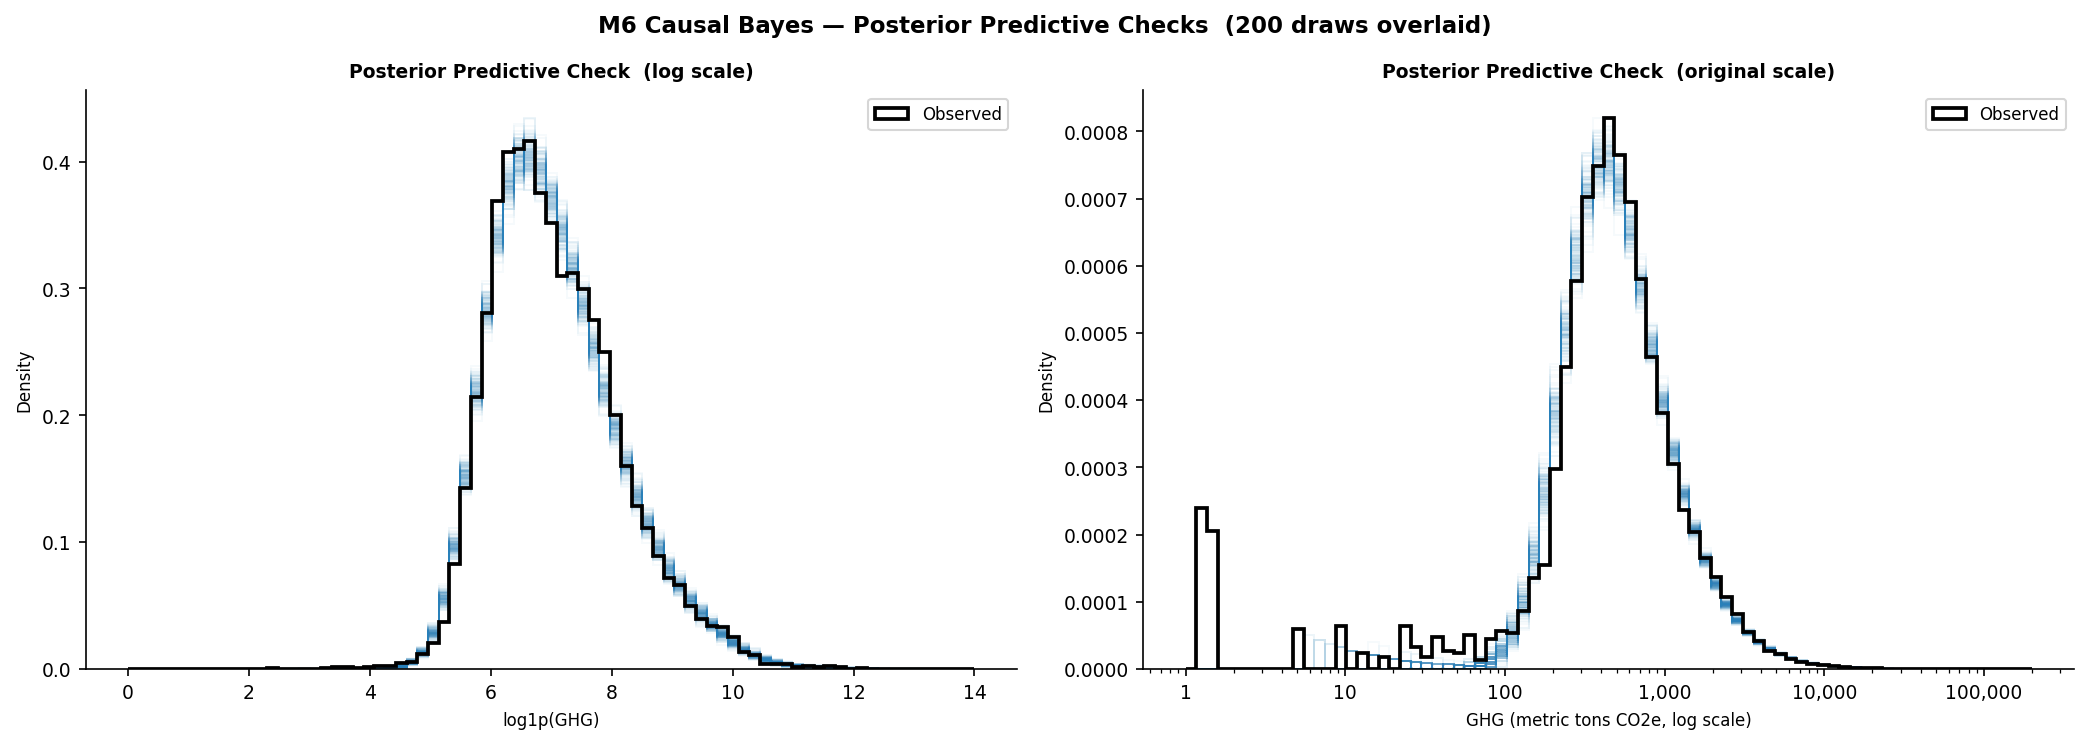
\includegraphics[width=0.95\linewidth]{figures/fig_ppc.png}
\caption*{\textbf{Figure 6.1. M6 posterior predictive check.} 200 datasets simulated from the posterior (blue) overlaid on the observed $\log_{1+}$(GHG) distribution (black), on the log scale (left) and the original scale with logarithmic axis (right). Author's analysis of Chicago Energy Benchmarking data.}
\end{figure}

\subsection{Global Parameter Posteriors}

Floor area and the temporal trend dominate the posterior, with substantial property-type heterogeneity and a precisely estimated residual scale. Table 6.1 reports all seven parameters with 89\% credible intervals; Figure 6.2 shows the forest plot.

\par\medskip\noindent
{\small\itshape \textbf{Table 6.1. M6 global parameter posteriors.} Posterior means and 89\% credible intervals for the seven scalar parameters of the generative model in Section 5.4. The four upstream slopes are the parameters of interest; $\bar{\alpha}$, $\sigma_\alpha$, and $\sigma$ are the hierarchy's location, spread, and residual scale. Author's analysis of Chicago Energy Benchmarking data.\par}
\nopagebreak\medskip\nopagebreak
{
\setlength{\tabcolsep}{7pt}
\renewcommand{\arraystretch}{1.15}
\begin{longtable}{lrrr}
\toprule
Parameter & Role & Mean & 89\% CI \\
\midrule
\endfirsthead
\toprule
Parameter & Role & Mean & 89\% CI \\
\midrule
\endhead
\bottomrule
\endlastfoot
$\bar{\alpha}$ & global intercept & +7.409 & [+7.304, +7.515] \\
$\sigma_\alpha$ & between-type SD & +0.483 & [+0.409, +0.568] \\
$\beta_A$ & log floor area & +0.979 & [+0.973, +0.985] \\
$\beta_B$ & log building count & +0.014 & [+0.002, +0.026] \\
$\beta_T$ & data year (standardised) & -0.145 & [-0.150, -0.140] \\
$\beta_Y$ & year built (standardised) & +0.047 & [+0.042, +0.052] \\
$\sigma$ & residual SD & +0.430 & [+0.427, +0.434] \\
\end{longtable}
}
\par\medskip

\textbf{Floor area, $\beta_A = 0.979$ [0.973, 0.985].} Floor area is the dominant parameter; with both outcome and regressor on the log scale, the coefficient is an elasticity: doubling floor area multiplies GHG by $2^{0.979} \approx 1.97$. The estimate is consistent with the near-unit elasticity that Stage 3 recovered by OLS from the upstream-to-mediator regressions (Table 4.3) and with the prior expectation the causal analyst encoded in Section 5.4. Three routes to the same quantity agree: the documented accounting identity, the nested OLS from Stage 3, and the full posterior all converge on near-unit scaling. The interval excludes 1.0, so the scaling is credibly sub-proportional: larger buildings emit slightly less per square foot, consistent with economies of scale in shared building systems.

\textbf{Data year, $\beta_T = -0.145$ [-0.150, -0.140].} The data-year slope is the strongest temporal signal and the best-identified parameter in the model: a one-standard-deviation increase in data year multiplies GHG by $\exp(-0.145) \approx 0.865$; with the panel spanning 2014--2023, this corresponds to a decline of roughly 5--6 percent per year. The sign and magnitude are consistent with the mechanism Stage 3 identified when it lifted the data year out of $X_o$: the year-on-year fall in the eGRID electricity emission factor (Section 4.4), compounded by efficiency improvements in the stock itself. The tested DAG predicted a real temporal edge into the outcome; the posterior quantifies it.

\textbf{Building count, $\beta_B = 0.014$ [0.002, 0.026].} The building-count slope is small but credibly positive: holding total floor area fixed, properties spread across more buildings emit marginally more, with doubling the count adding roughly 1\%. A plausible reading is common-area and circulation overhead that accrues per building rather than scaling with floor area. The interval sits entirely above zero but the effect is not a dominant driver.

\textbf{Year built, $\beta_Y = +0.047$ [0.042, 0.052].} Newer construction is associated with slightly higher emissions after controlling for size, type, and reporting year. The sign may appear counterintuitive; one plausible reading is that newer buildings in the benchmarked stock are more complex developments with higher equipment loads and year-round conditioning, a residual composition effect within property types. The contrast with $\beta_T$ is informative: operational efficiency improves over reporting years even as design complexity rises in newer construction. The two parameters separate the two mechanisms because the tested DAG carries them on different nodes.

\textbf{Location, spread, and residual.} The global intercept $\bar{\alpha} = 7.409$ implies a typical benchmarked building at mean covariates emits $\exp(7.409) - 1 \approx 1{,}649$ metric tons CO$_2$e annually. The between-type standard deviation $\sigma_\alpha = 0.483$ is well separated from zero, so property type carries substantial information beyond size and age; Section 6.3 unpacks it. The residual scale $\sigma = 0.430$ is the irreducible within-type variation: buildings of the same type, size, age, and year still vary by a multiplicative factor of roughly 0.65 to 1.54 around the conditional mean. This is the quantitative floor under the predictive results of Section 5: a residual SD of 0.43 log units is consistent with the observed MdAPE near 21\%, and it is why Section 5.5 treated very low cross-validation error as a diagnostic signal rather than an achievement. Occupancy, operational schedules, and equipment age are not observed, and the model prices that honestly.

\begin{figure}[tbp]
\centering
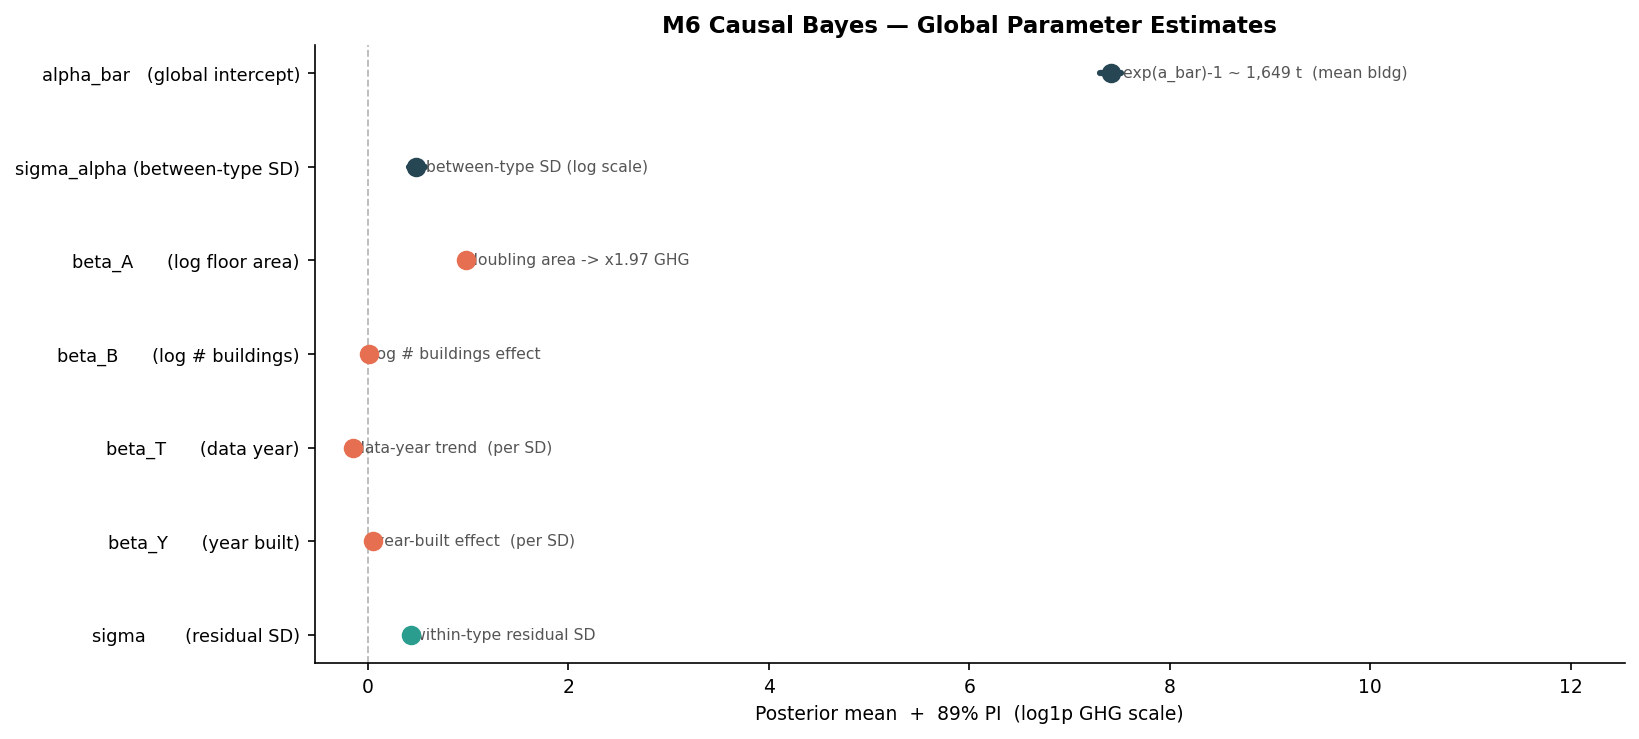
\includegraphics[width=0.95\linewidth]{figures/fig_coef_forest.png}
\caption*{\textbf{Figure 6.2. M6 global parameter estimates.} Forest plot of the seven scalar posteriors with 89\% credible intervals and back-transformed interpretations. Author's analysis of Chicago Energy Benchmarking data.}
\end{figure}

\subsection{The Property-Type Hierarchy}

Property type spans a 22-fold emissions range beyond what size, age, and reporting year explain: the 55 estimated intercepts $\alpha_j = \bar{\alpha} + \delta_j \sigma_\alpha$ run from Data Center at $+9.352$ [9.189, 9.515] down to Repair Services at $+6.234$ [6.015, 6.452], a spread of 3.1 log units. Figure 6.3 ranks all 55 types represented in the compliant training set (of the 63 the dataset records; Section 4.1).

The ordering is consistent with engineering knowledge rather than statistical accident. Data centres run power densities an order of magnitude above typical commercial space; laboratories ($+8.386$) carry ventilation and fume-hood loads around the clock; supermarkets ($+8.286$) run continuous refrigeration. At the bottom, repair services and distribution centres combine low occupancy density with intermittent conditioning. A flat model that ignored property type would be systematically wrong across this entire range, which is the empirical justification for the hierarchical structure.

The interval widths encode data availability, and that is partial pooling working as intended. Frequently reported types such as Laboratory have intervals about 0.10 log units wide; rare types carry far wider intervals: Repair Services spans 0.44 log units and Distribution Center spans 0.83. Each is accordingly shrunk toward the global mean rather than extrapolated from sparse local data. Data Center keeps a high posterior mean despite few observations because the signal is strong enough to overcome the pooling.

\begin{figure}[tbp]
\centering
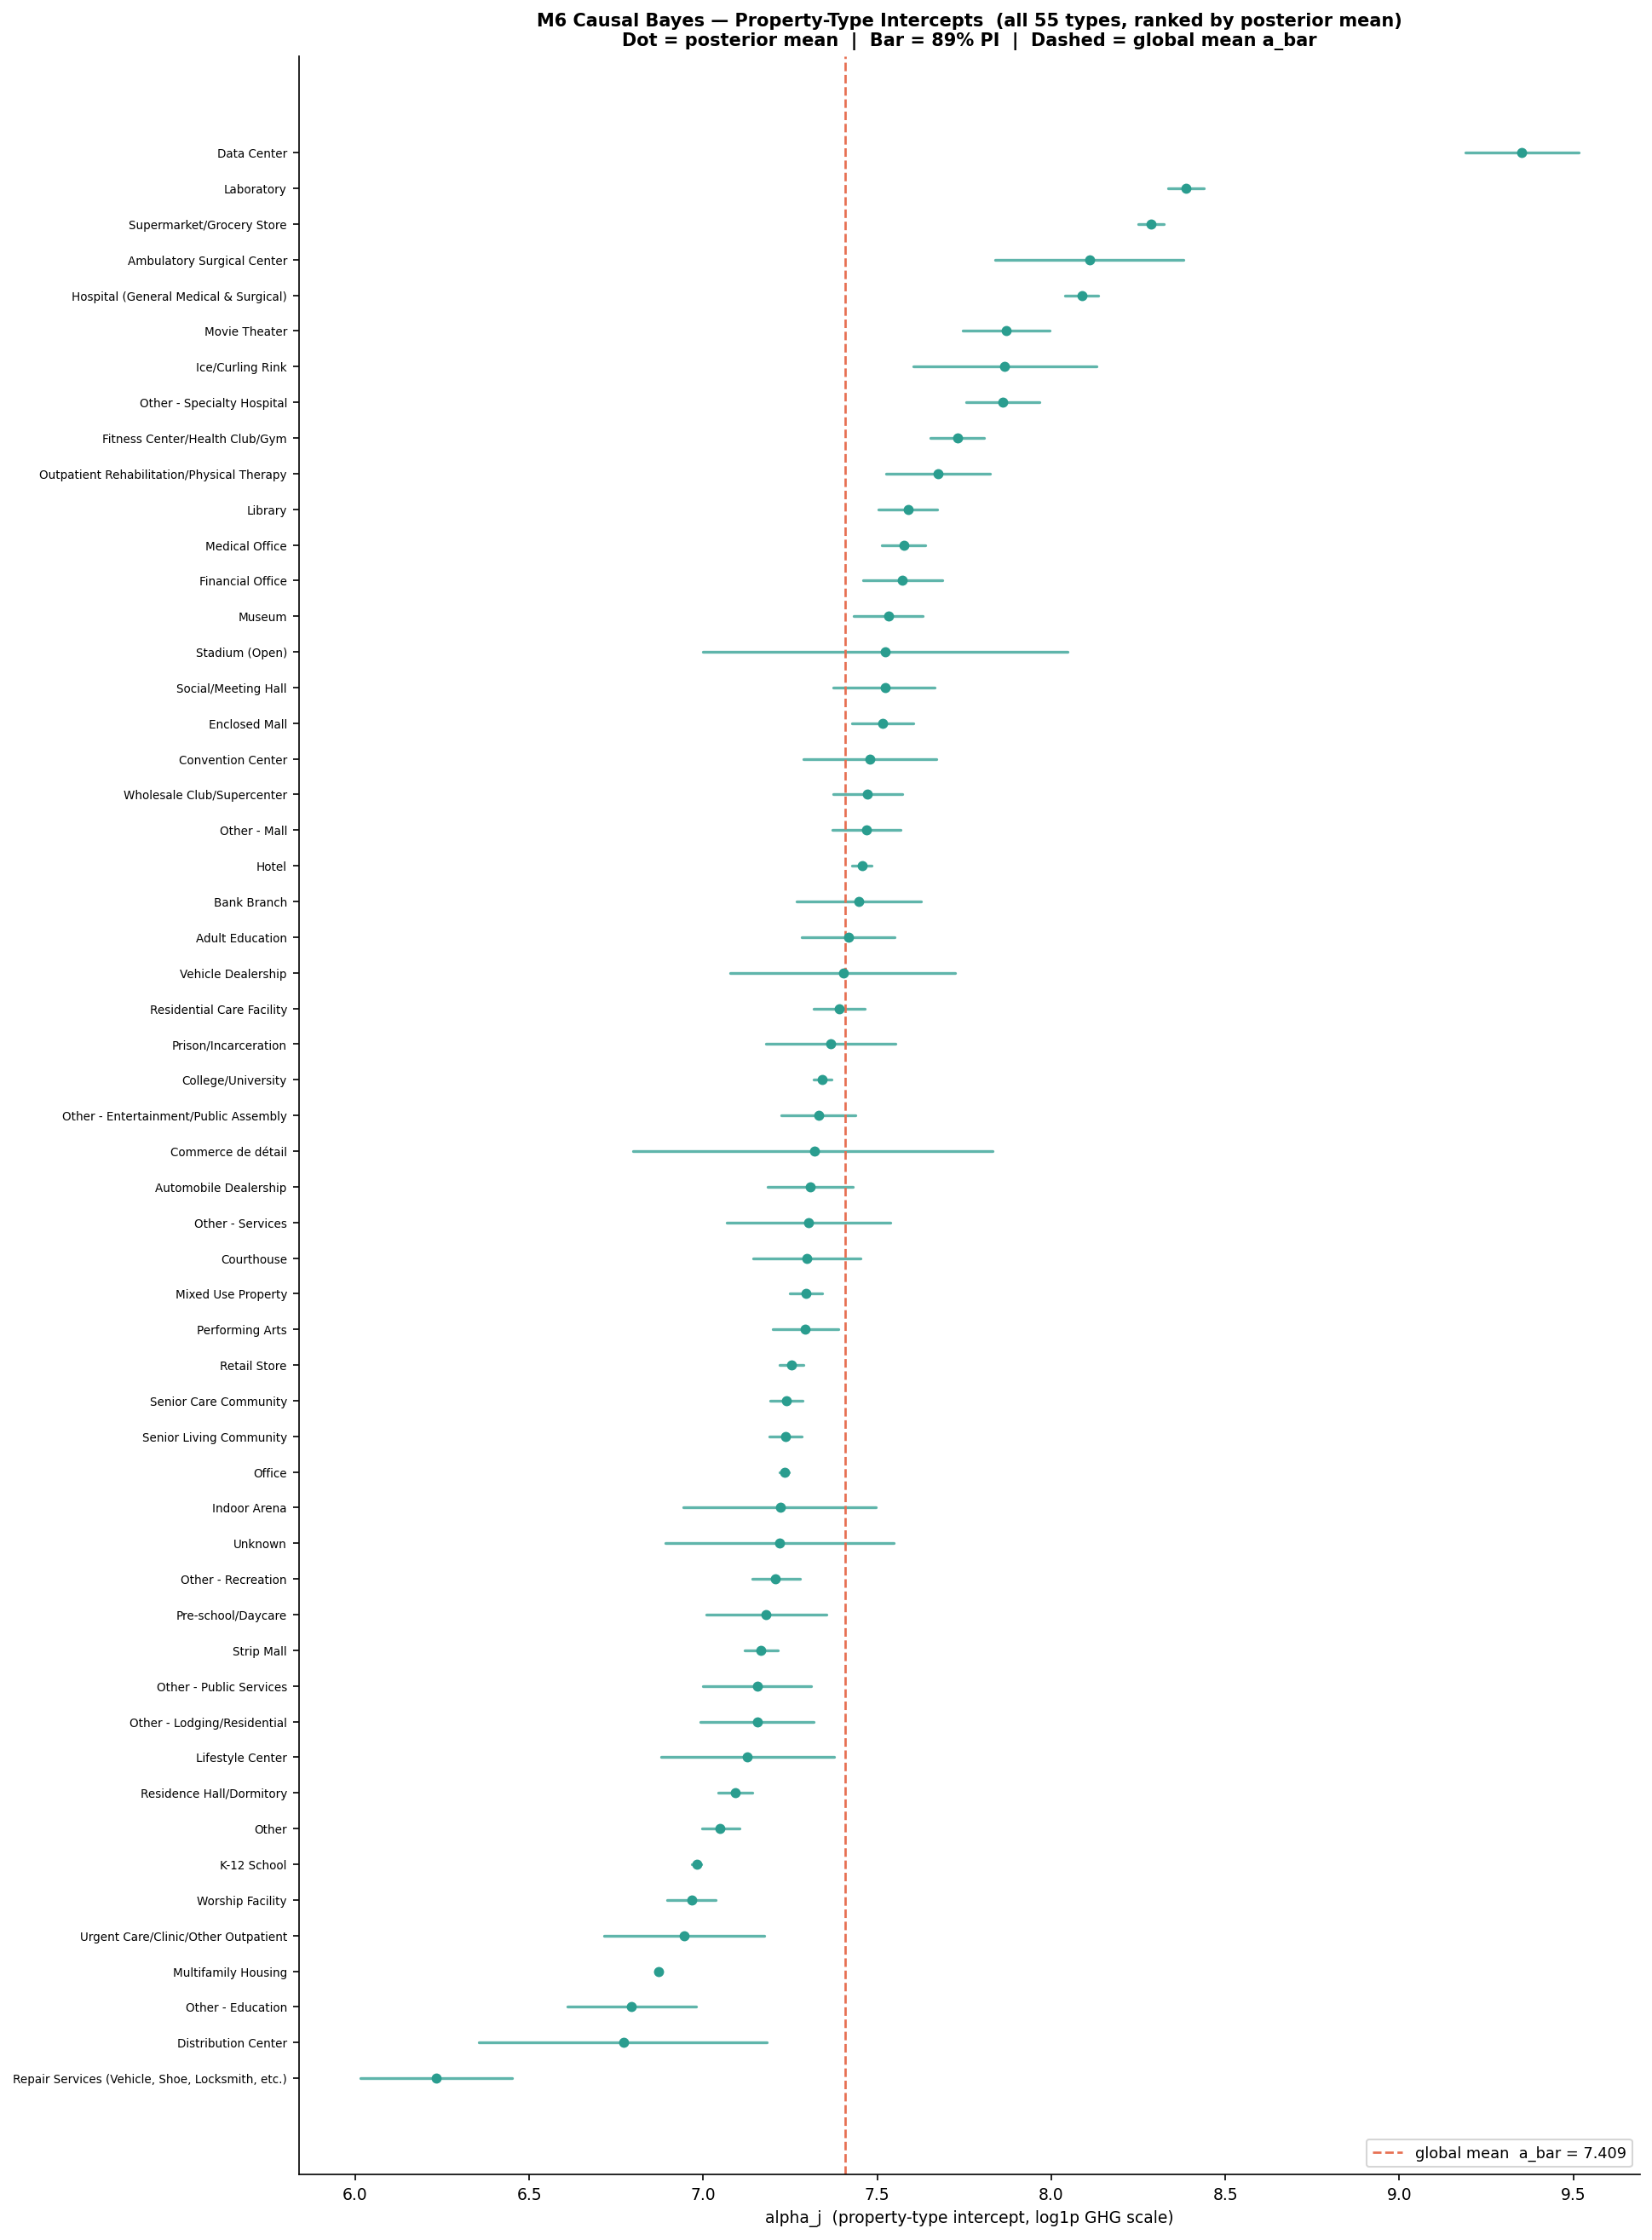
\includegraphics[width=0.8\linewidth]{figures/fig_type_intercepts.png}
\caption*{\textbf{Figure 6.3. Property-type intercepts, all 55 types.} Ranked posterior means with 89\% credible intervals for $\alpha_j$; the dashed line marks the global mean $\bar{\alpha}$. Interval width tracks how often each type appears in the compliant training set. Author's analysis of Chicago Energy Benchmarking data.}
\end{figure}

\subsection{Deployment Inference for the Non-Compliant Stock}

The deployment exercise of Section 5.6 reported point predictions; the posterior adds their uncertainty. M6 is applied to the 5,510 building-year records that never reported under the ordinance, using only their upstream features, the only inputs that exist for a non-reporting building. The posterior predictive median is 1,043 metric tons CO$_2$e against an observed compliant median of 1,018, a difference of 2.5\%, with an 89\% interval for an individual building of [495, 2,103] (Figure 6.4).

Two features of this result deserve emphasis. First, the interval is wide, roughly a factor of four, and deliberately so: without observed energy use, the residual scale $\sigma$ and the type uncertainty propagate through the posterior predictive in full, and a narrower interval would be a false promise rather than a better model. Second, non-compliant buildings predict at essentially the same emission level as compliant ones. Within the limits stated in Section 5.6 (no ground truth exists for these buildings), this is the pattern the tested DGP predicts: compliance is determined by the gate variables, not by emissions, so once the upstream features are conditioned on, non-reporting buildings should look like reporting ones. The result is consistent with selection rather than with a systematically cleaner non-reporting stock.

The per-type medians show meaningful heterogeneity beneath the aggregate: K-12 schools at 676 t and multifamily housing at 893 t sit below the global level, while mixed-use properties (2,117 t), college and university buildings (1,360 t), and offices (1,298 t) sit above it. One data feature matters for interpretation: 3,924 of the 5,510 non-compliant records (71\%) carry an Unknown property type, because a building that never filed has no recorded type. These buildings receive the global intercept with full between-type uncertainty, and their deployment median (1,021 t) accordingly sits near the global level. That is the model behaving correctly under missing type information, not a separate finding about unknown-type buildings.

\begin{figure}[tbp]
\centering
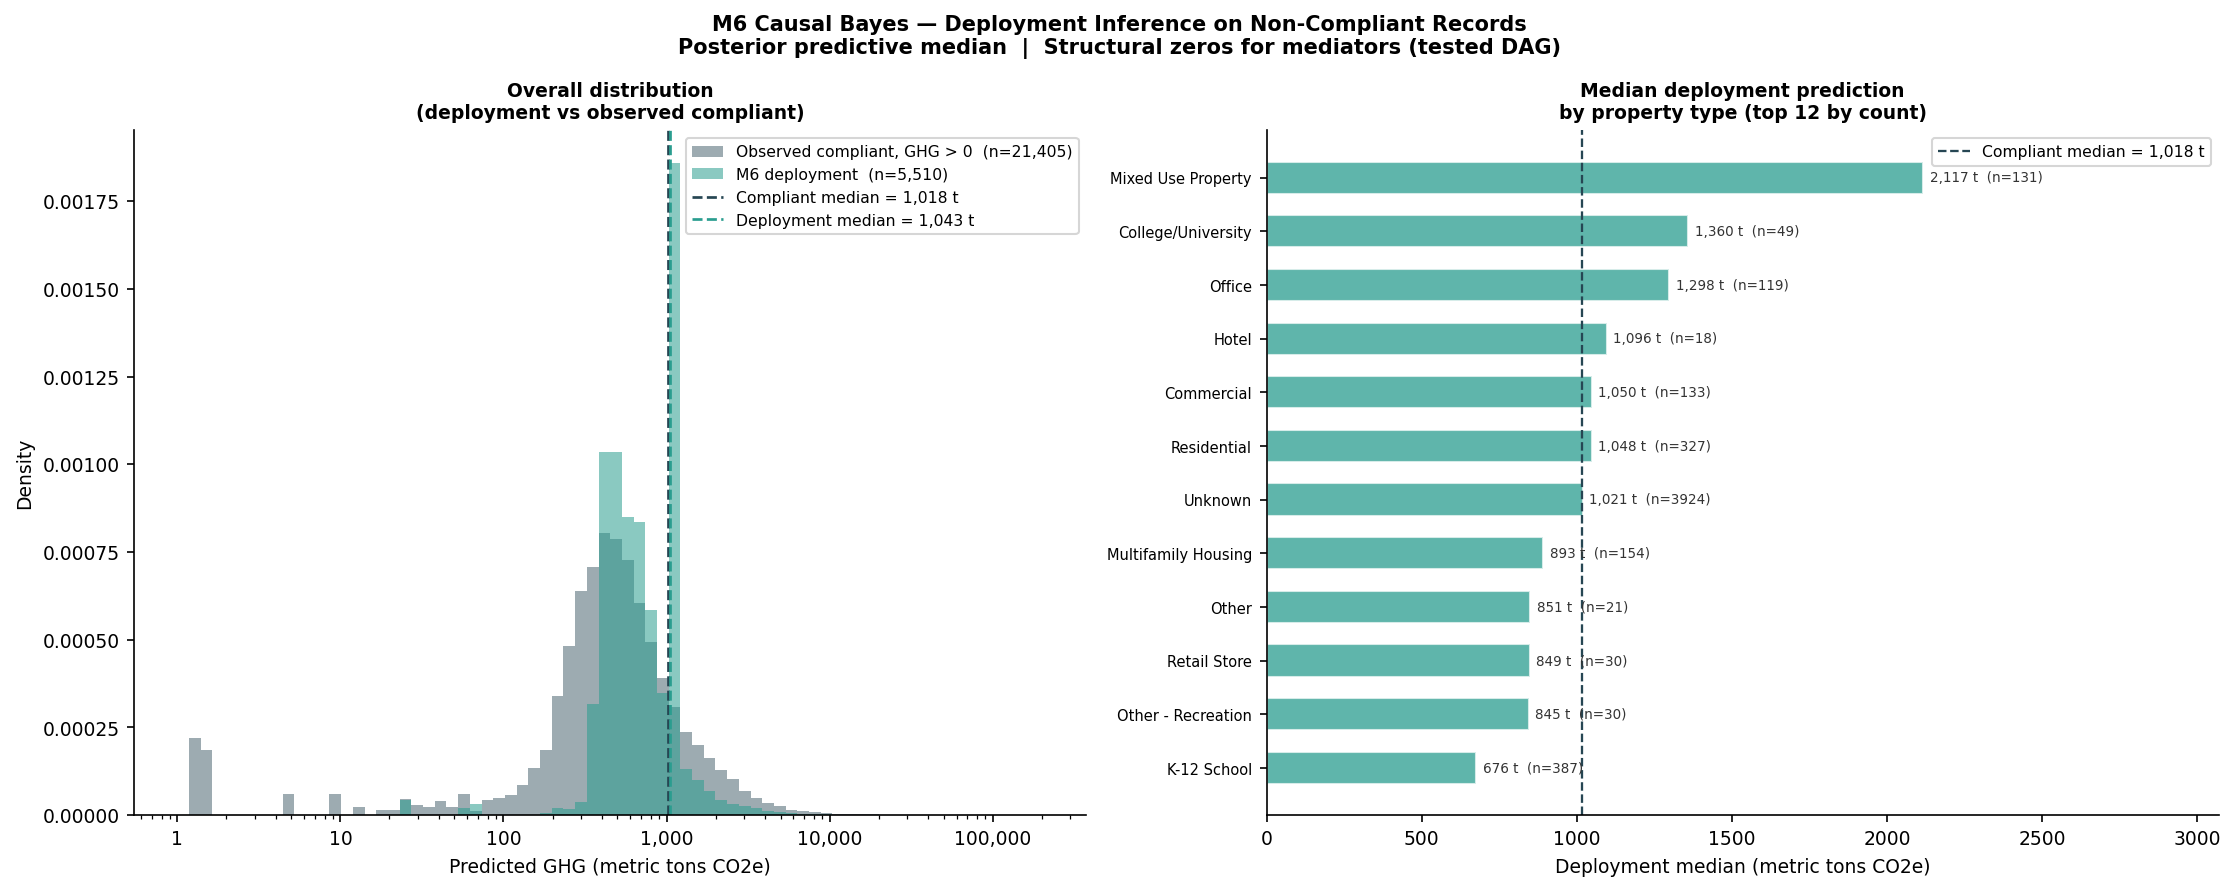
\includegraphics[width=0.95\linewidth]{figures/fig_m6_deployment.png}
\caption*{\textbf{Figure 6.4. Deployment inference for 5,510 non-compliant building-year records.} Left: posterior predictive distribution for the non-compliant stock against the observed compliant distribution, with medians marked (1,043 vs 1,018 metric tons CO$_2$e). Right: per-type deployment medians for the twelve most common non-compliant property types. Author's analysis of Chicago Energy Benchmarking data.}
\end{figure}

\subsection{Sensitivity Analysis}

The posteriors above rest on two analyst-controlled inputs: the prior specification and the IPW trim cap. The sensitivity analysis tests whether the section's findings depend on either. The design is committed ex ante, in the same spirit as the predictions of Section 5.5: the four parameters of interest ($\beta_A$, $\beta_T$, $\sigma_\alpha$, $\sigma$) and the review criterion are declared before any alternative model is fitted, so the analysis cannot select favourable specifications after the fact. The criterion flags a parameter for review when its posterior mean shifts by more than 20\% of the base 89\% credible interval half-width. The intercept prior $\bar{\alpha} \sim \text{Normal}(7.0, 1.0)$ is not varied, since it is anchored to the observed log-GHG mean of 7.08 rather than chosen freely.

Each dimension is varied independently around the base specification, which is loaded from the saved experiment trace rather than re-fitted, so the base column is identical to Table 6.1 by construction. On the prior dimension, the slope priors are tightened to $\text{Normal}(0, 0.25)$ and loosened to $\text{Normal}(0, 1.00)$ against the base $\text{Normal}(0, 0.50)$, with the scale priors varied in step. On the weighting dimension, the raw inverse propensity weights are capped at the 95th, 99th (base; \cit{colehernan2008}{Cole \& Hernán, 2008}), and 99.9th percentiles. All four alternative fits use the identical sampling specification as M6 and all converge cleanly: zero divergent transitions in every run, $\hat{R}_{\max} \leq 1.006$ across the new fits, and $\text{ESS}_{\min} \geq 460$.

The three caps produce maximum normalised weights of 1.166, 1.322, and 2.750, and the asymmetry is informative. Tightening from the 99th to the 95th percentile changes the maximum weight by only 12\%, because the weight distribution is compact in that region. Loosening to the 99.9th percentile more than doubles it, admitting a small number of buildings whose estimated compliance propensity falls below roughly 35\%, predominantly very small buildings and atypical property types, each now carrying about twice the influence of an average observation. The lenient cap is included as a deliberate stress test, not as a plausible alternative.

Table 6.2 summarises the outcome. Against prior specification, all four parameters are stable: the largest shift anywhere is 3.2\% of the interval half-width, and $\beta_A$ and $\beta_T$ are identical to three decimal places across all three prior widths. With 21,406 observations the likelihood dominates any reasonable prior; halving or doubling the prior scales produces no detectable change. The largest (still negligible) prior sensitivity belongs to $\sigma_\alpha$, as expected: the between-type standard deviation is informed by the 55 types rather than the 21,406 buildings, so its effective sample is the smallest in the model.

\par\medskip\noindent
{\small\itshape \textbf{Table 6.2. Sensitivity of the four parameters of interest.} Maximum shift in posterior mean across the alternative specifications on each dimension, expressed as a percentage of the base 89\% credible interval half-width; the review threshold is 20\%. Author's analysis of Chicago Energy Benchmarking data.\par}
\nopagebreak\medskip\nopagebreak
{
\setlength{\tabcolsep}{7pt}
\renewcommand{\arraystretch}{1.15}
\begin{longtable}{lrrr}
\toprule
Parameter & Prior shift (max) & IPW shift (max) & Assessment \\
\midrule
\endfirsthead
\toprule
Parameter & Prior shift (max) & IPW shift (max) & Assessment \\
\midrule
\endhead
\bottomrule
\endlastfoot
$\beta_A$ & 3.2\% & 29.0\% (see text) & robust \\
$\beta_T$ & 1.0\% & 11.0\% & robust \\
$\sigma_\alpha$ & 3.2\% & 1.2\% & robust \\
$\sigma$ & 0.5\% & 11.3\% & robust \\
\end{longtable}
}
\par\medskip

Against the IPW trim cap, three of the four parameters again move by at most 11.3\% of the half-width, and $\beta_T$ is the strongest result in the analysis: the data-year trend is identical to three decimal places under every cap, because a temporal signal that operates across all buildings and all years cannot be redistributed by reweighting individual observations. The one flag is $\beta_A$ under the lenient 99.9th-percentile cap, at 29\% of the half-width. The 29\% figure is inflated by the denominator, not the numerator: the absolute shift is 0.0018 (posterior mean 0.979 to 0.977), the half-width it is measured against is 0.006, and the implied change in the floor-area doubling effect is from $\times 1.971$ to $\times 1.968$, a 0.15\% difference with no analytical consequence. The mechanism is also interpretable: the extreme weights upweight small, low-propensity buildings, marginally reducing the leverage of large buildings and with it the estimated elasticity. Figure 6.5 shows the full comparison; on every panel the markers for the three specifications overlap rather than spread.

The joint conclusion is that the findings of Sections 6.2 through 6.4 are properties of the data and the tested structure, not artefacts of prior choice or weight trimming. The elasticity near one, the decarbonisation trend, the 22-fold type heterogeneity, and the residual floor all survive every specification tested, and the 99th-percentile trim of the base model, adopted from \cit{colehernan2008}{Cole and Hernán (2008)}, emerges corroborated: the aggressive and lenient caps bracket it and produce essentially the same model.

\begin{figure}[tbp]
\centering
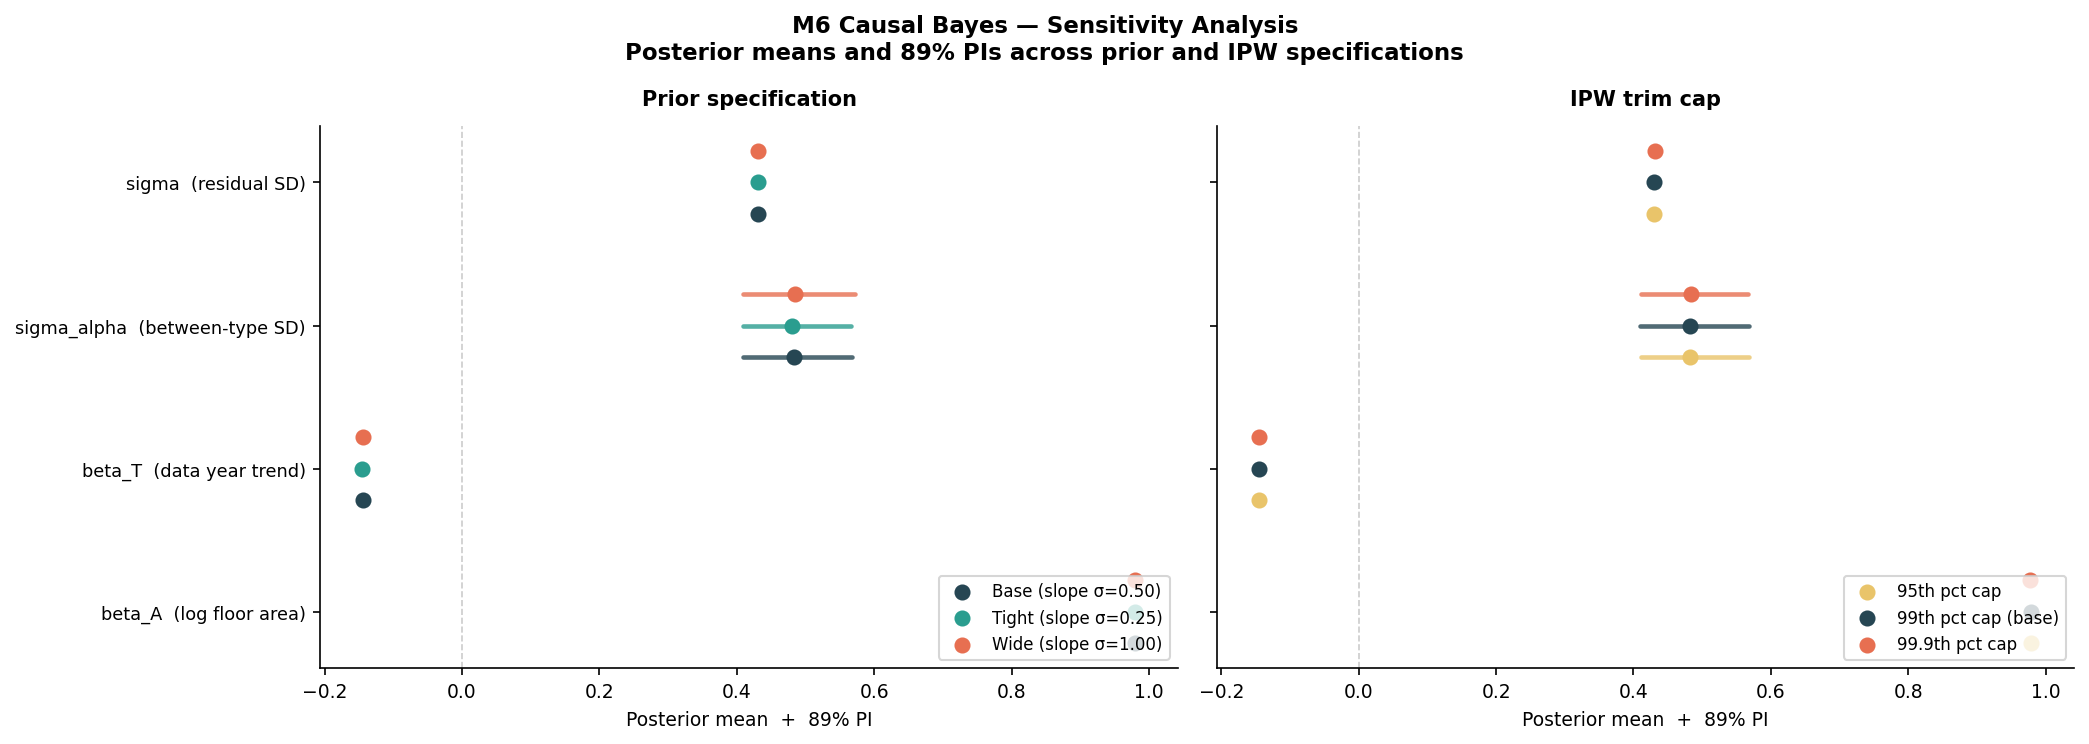
\includegraphics[width=0.95\linewidth]{figures/fig_sensitivity_forest.png}
\caption*{\textbf{Figure 6.5. Sensitivity forest plot.} Posterior means and 89\% credible intervals for $\beta_A$, $\beta_T$, $\sigma_\alpha$, and $\sigma$ across all specifications. Left: prior sensitivity (tight, base, wide; IPW fixed at the 99th percentile). Right: IPW sensitivity (95th, 99th, 99.9th percentile caps; priors fixed at base). Overlapping markers indicate robustness. Author's analysis of Chicago Energy Benchmarking data.}
\end{figure}


\FloatBarrier
\section{Counterfactual Analysis}

Section 3.4 promised that a structure surviving Stage 3 licenses the third rung of the ladder, and this section redeems that promise on the fitted model. Three queries are evaluated. The first converts the posterior trend $\beta_T$ into a calendar-year decarbonisation rate and measures it against policy targets (Section 7.1). The second and third are the counterfactual queries of Section 3.4: what each building's compliance standing would be were the panel observed in 2030 (Section 7.2), and what each building would emit had it been built in 2010 (Section 7.3).

Every number in this section is an analytical function of the saved M6 posterior: each query substitutes one feature value in the linear predictor of Section 5.4, holds all other covariates at their observed values, and re-evaluates across the 12,000 draws and 21,406 compliant records, with no new sampling. The object being manipulated is the fitted predictor

\[
\mu_i = \alpha_{j[i]} + \beta_A \tilde{a}_i + \beta_B \tilde{b}_i + \beta_T \tilde{t}_i + \beta_Y \tilde{y}_i,
\]

in the notation of Section 5.4, evaluated at each posterior draw. Because the predictor is linear, substituting one feature moves each record's log-scale prediction by exactly one coefficient times the feature's displacement, which is why every query in this section reduces to one matrix operation per draw. Both intervened features sit outside the gate, which keys on floor area and property type alone, so the interventions leave each unit's compliance untouched; this is the action step of Section 3.4, and the queries concern the world layer alone.

\subsection{Decarbonisation Pace against Policy Benchmarks}

The posterior trend becomes a policy-readable rate once the standardisation is undone. $\beta_T$ measures the log-change per standard deviation of the data year, and one calendar year is $1/s_t$ of that unit, with $s_t = 2.590$ the panel's year standard deviation. The per-year rate is therefore

\[
r = \frac{\beta_T}{s_t} = \frac{-0.1447}{2.590} = -0.0559 \text{ log units per year},
\]

which exponentiates to $e^r - 1 = -5.43$ percent per year; applying the same map to every posterior draw gives the 89\% credible interval $[-5.61, -5.26]$ percent. This is the same parameter Section 6.2 reported on the standardised scale; the conversion changes its units, not its evidence.

The estimated pace clears the city's official target. A sustained rate $r$ reaches a fraction $q$ of the baseline after $\ln(q)/r$ years; equivalently, reaching fraction $q$ in $n$ years requires a rate of $\ln(q)/n$. The 2022 Chicago Climate Action Plan commits the city to a 62 percent reduction in citywide emissions by 2040 against a 2017 baseline (\cit{city2022}{City of Chicago, 2022}), which over that 23-year window requires $\ln(0.38)/23 = -0.0421$ log units per year. The estimated rate of $-0.0559$ exceeds it: sustained from 2017 to 2040, the trend delivers $1 - e^{23r} \approx 72$ percent. The comparison is indicative rather than conclusive, since the plan's target covers all sectors while the estimate describes the benchmarked building stock alone.

Full decarbonisation is a different matter, and a stricter benchmark shows where the trend alone gives out. At the estimated rate, an 80 percent reduction ($q = 0.20$) from the 2023 level takes $\ln(0.20)/(-0.0559) \approx 29$ years, arriving around 2052. A stylised net-zero-by-2040 benchmark, operationalised as a 99 percent reduction since the multiplicative scale cannot express zero, requires $r^\star = \ln(0.01)/17 = -0.2709$ log units per year over the seventeen years from 2023. That is $-23.73$ percent per year, roughly 4.4 times the estimated pace, leaving a shortfall of $r^\star - r = -0.2150$ log units per year (Figure 7.1). The comparison is between rates of change, not levels: the estimated rate is identified from the panel structure of the data, and the required rate follows from the target and the horizon, so the gap measures how far the observed dynamics are from the dynamics the target presumes.

Two qualifications bound the finding. The projection assumes the estimated trend persists unchanged to 2040, and the trend itself bundles the fall in the grid emission factor (Section 4.4) with efficiency change in the stock, so it is not a building-efficiency rate alone. Within those limits the rate is the best-defended number in the posterior: Section 6.5 found $\beta_T$ identical to three decimal places under every prior and weighting specification tested.

\begin{figure}[tbp]
\centering
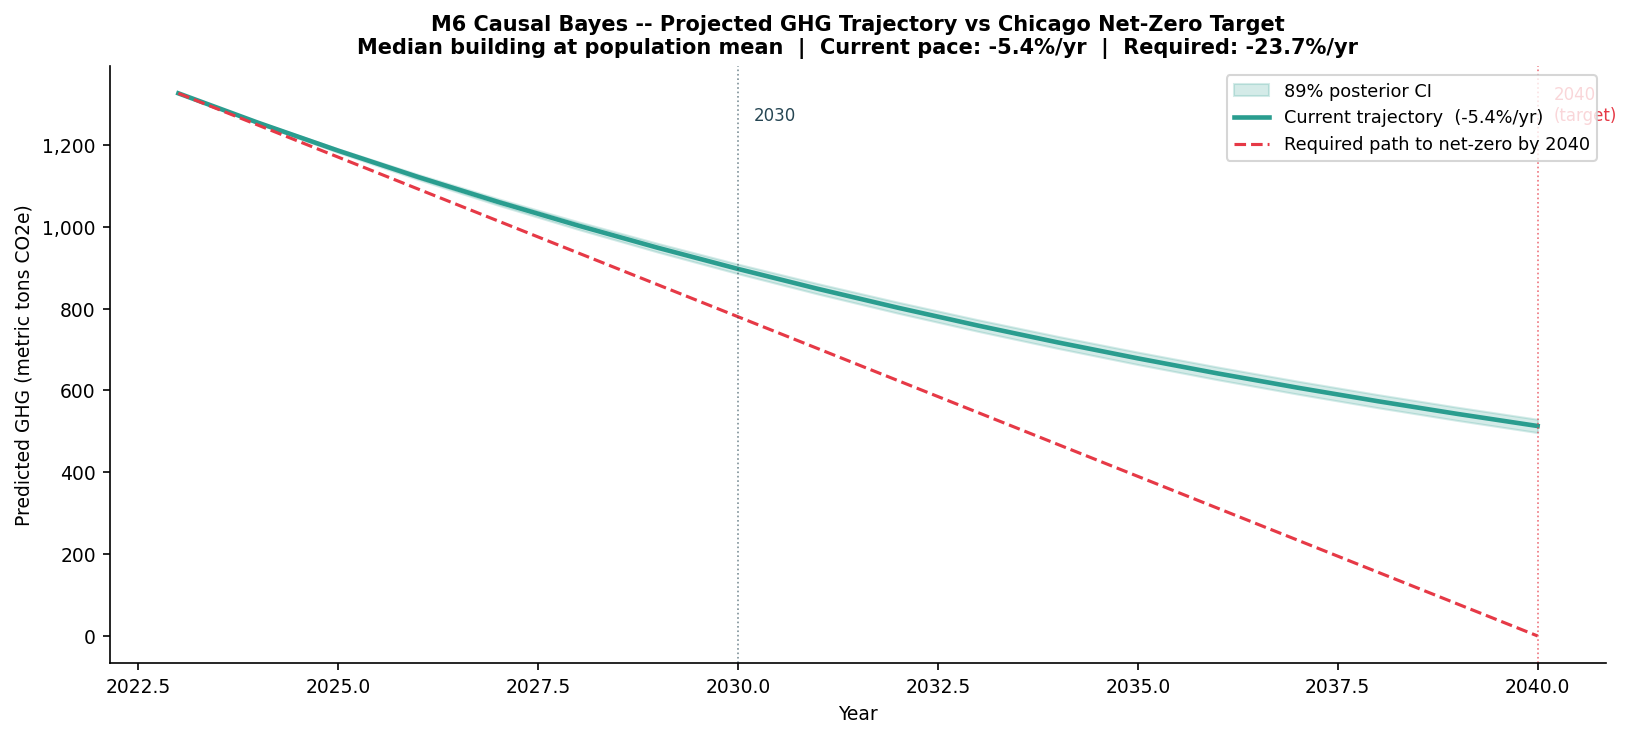
\includegraphics[width=0.95\linewidth]{figures/fig_trend.png}
\caption*{\textbf{Figure 7.1. Projected GHG trajectory against the stylised 2040 net-zero benchmark.} Posterior trajectory for a building at the population mean of the covariates, projected from 2023 at the estimated rate of $-5.4$ percent per year with its 89\% credible band, against the path required for full decarbonisation by 2040; the benchmark is stricter than the city's official 62 percent target (see text). Author's analysis of Chicago Energy Benchmarking data.}
\end{figure}

\subsection{Counterfactual 1: Compliance Risk in 2030}

The first counterfactual asks which buildings the trend alone will carry below a compliance threshold by 2030. The query sets the data year to 2030 for every record while holding size, type, vintage, and building count at observed values: the counterfactual year standardises to $\tilde{t}^\star = (2030 - 2019.1)/s_t = 4.21$, and replacing $\tilde{t}_i$ in $\mu_i$ shifts each record's log-scale prediction by $\beta_T(\tilde{t}^\star - \tilde{t}_i)$. The counterfactual year lies seven years past the panel's edge, so the query inherits the trend-persistence qualification of Section 7.1. For each posterior draw the residual is then added and the outcome back-transformed, $y^\star_i \sim \text{Normal}(\mu^\star_i, \sigma)$ with $\text{GHG}^\star_i = e^{y^\star_i} - 1$, and the compliance probability is the fraction of draws falling at or below the threshold $\tau$:

\[
P_i = P\big(\text{GHG}_i \leq \tau \mid do(\text{data year} = 2030)\big) = \frac{1}{12{,}000} \sum_{d=1}^{12{,}000} \mathbf{1}\{\text{GHG}^\star_{i,d} \leq \tau\}.
\]

Because the draws span the parameter posterior and the residual scale $\sigma$ jointly, $P_i$ carries both parameter uncertainty and building-level idiosyncrasy, and compliance becomes a probability rather than a verdict.

The threshold and the bands are stylised inputs, chosen for illustration rather than drawn from the ordinance. The threshold $\tau = 546$ metric tons CO$_2$e is the 25th percentile of observed GHG in the compliant training set, standing in for a performance standard; records are classified on-track when $P_i > 0.80$, high-risk when $P_i < 0.20$, and uncertain between. The contribution is the machinery, which applies unchanged to whatever threshold a regulator specifies.

Table 7.1 shows the portfolio splitting into three comparable blocks. The trend alone carries 35.4 percent of records on-track, leaves 37.1 percent at high risk even by 2030, and places 27.5 percent in the uncertain band; the median compliance probability across all records is 0.526, barely better than even odds. The uncertain band is the policy-relevant population, since these are the marginal cases where a targeted intervention could change the classification, while the high-risk block will not reach the threshold on trend continuation alone. The shares are over building-year records rather than buildings, so a building weighs in proportion to its reporting tenure.

\par\medskip\noindent
{\small\itshape \textbf{Table 7.1. Compliance classification under the 2030 counterfactual.} Records classified by posterior probability of falling below the 546 t CO$_2$e threshold when the data year is set to 2030. Author's analysis of Chicago Energy Benchmarking data.\par}
\nopagebreak\medskip\nopagebreak
{
\setlength{\tabcolsep}{7pt}
\renewcommand{\arraystretch}{1.15}
\begin{longtable}{lrrr}
\toprule
Classification & Criterion & Records & Share \\
\midrule
\endfirsthead
\toprule
Classification & Criterion & Records & Share \\
\midrule
\endhead
\bottomrule
\endlastfoot
On-track & $P_i > 0.80$ & 7,586 & 35.4\% \\
Uncertain & $0.20 \leq P_i \leq 0.80$ & 5,887 & 27.5\% \\
High-risk & $P_i < 0.20$ & 7,933 & 37.1\% \\
\end{longtable}
}
\par\medskip

This per-record probability is an output the point-prediction pipelines of Section 5 do not deliver. A point prediction combined with a hard threshold returns a single binary verdict per record; the posterior returns a probability, which is what risk-ranked targeting requires and what separates the marginal records from the firmly off-track ones.

\begin{figure}[H]
\centering
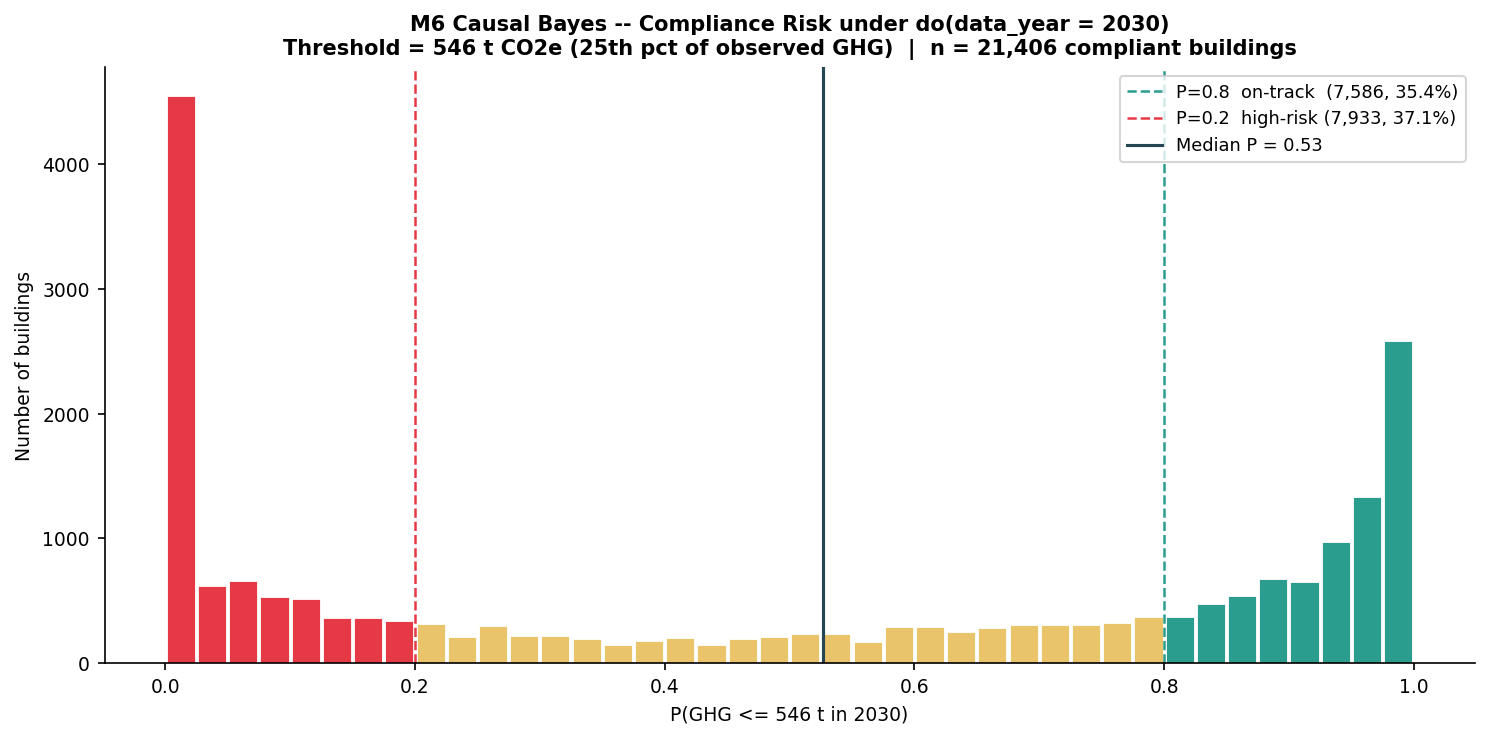
\includegraphics[width=0.95\linewidth]{figures/fig_cf1_compliance.png}
\caption*{\textbf{Figure 7.2. Compliance risk under the 2030 counterfactual.} Distribution of $P(\text{GHG} \leq 546\ \text{t})$ across the 21,406 compliant records with the 0.20 and 0.80 classification bounds and the median probability marked. Author's analysis of Chicago Energy Benchmarking data.}
\end{figure}

\subsection{Counterfactual 2: Vintage Reassignment}

The second counterfactual reassigns every building's construction year to 2010, against an actual mean vintage of 1964, and compares each record's predicted emissions under the two regimes. The disturbance enters both regimes identically and cancels from the contrast on the log scale, so the comparison requires only the posterior over the equations; this is the three-step computation of Section 3.4 (\cit{pearl2009}{Pearl, 2009}; \cit{pearletal2016}{Pearl, Glymour \& Jewell, 2016, Ch. 4}) with the action falling on the vintage node. Linearity makes the contrast exact: the factual and counterfactual predictors differ in the vintage term alone, so for each posterior draw

\[
\mu^{CF}_i - \mu^{F}_i = \beta_Y\,(\tilde{y}^\star - \tilde{y}_i) = \beta_Y \cdot \frac{2010 - v_i}{s_y}.
\]

Here $v_i$ is the record's actual construction year, $s_y = 37.4$ is the training-set standard deviation of year built, and $\tilde{y}^\star = (2010 - 1964.3)/s_y = 1.22$ is the counterfactual vintage on the training standardisation. The reported difference is taken on the original scale with the disturbance at its central value, $\Delta_i = (e^{\mu^F_i} - 1) - (e^{\mu^{CF}_i} - 1)$, and summarised per record across the 12,000 draws.

The result runs against the intuition that newer means cleaner. The median per-record difference, factual minus counterfactual, is $-48$ metric tons CO$_2$e, and the 89\% credible interval for a typical record is $[-53, -42]$: the 2010-vintage counterfactual is predicted to emit more, not less. The direction is near-uniform, with 90.2 percent of records showing a credible increase, 8.8 percent a credible reduction, and 1.0 percent no credible effect (Figure 7.3). The mean difference of $-115$ t exceeds the median because the deltas scale with building size. The magnitude follows directly from the Section 6.2 posterior: a building of mean vintage moves 1.22 standard deviations, which at $\beta_Y = 0.047$ shifts the log scale by $0.047 \times 1.22 \approx 0.057$ and multiplies predicted emissions by $e^{0.057} \approx 1.06$; six percent of a median-sized building is some 50 to 60 t, consistent with the reported median.

The sign is counterintuitive only if $\beta_Y$ is read as a building-code efficiency effect, which the tested structure says it is not. The DAG carries reporting year and construction year on separate nodes, and Section 6.2 showed the posterior separating them: $\beta_T$ absorbs the year-on-year efficiency improvement, so what remains in $\beta_Y$ is the cross-sectional composition of vintage cohorts, consistent with the reading given there that newer construction in the benchmarked stock houses more energy-intensive operations. Under that reading, reassigning a 1960s building to 2010 moves it into a more intensive cohort, and the model predicts higher emissions accordingly.

Two implications follow, one for policy and one for method. For policy, vintage is a poorly targeted instrument: a programme that rewards newer construction as such would reward the more intensive cohort, and area-normalised intensity standards by property type are the better-aimed lever. For method, this query is not a retrofit-impact estimator and should not be read as one, because a retrofit operates through the energy mediators, which are compliance-gated and outside the upstream feature set; estimating that effect requires the mediator layer and is beyond this paper's scope.

\begin{figure}[H]
\centering
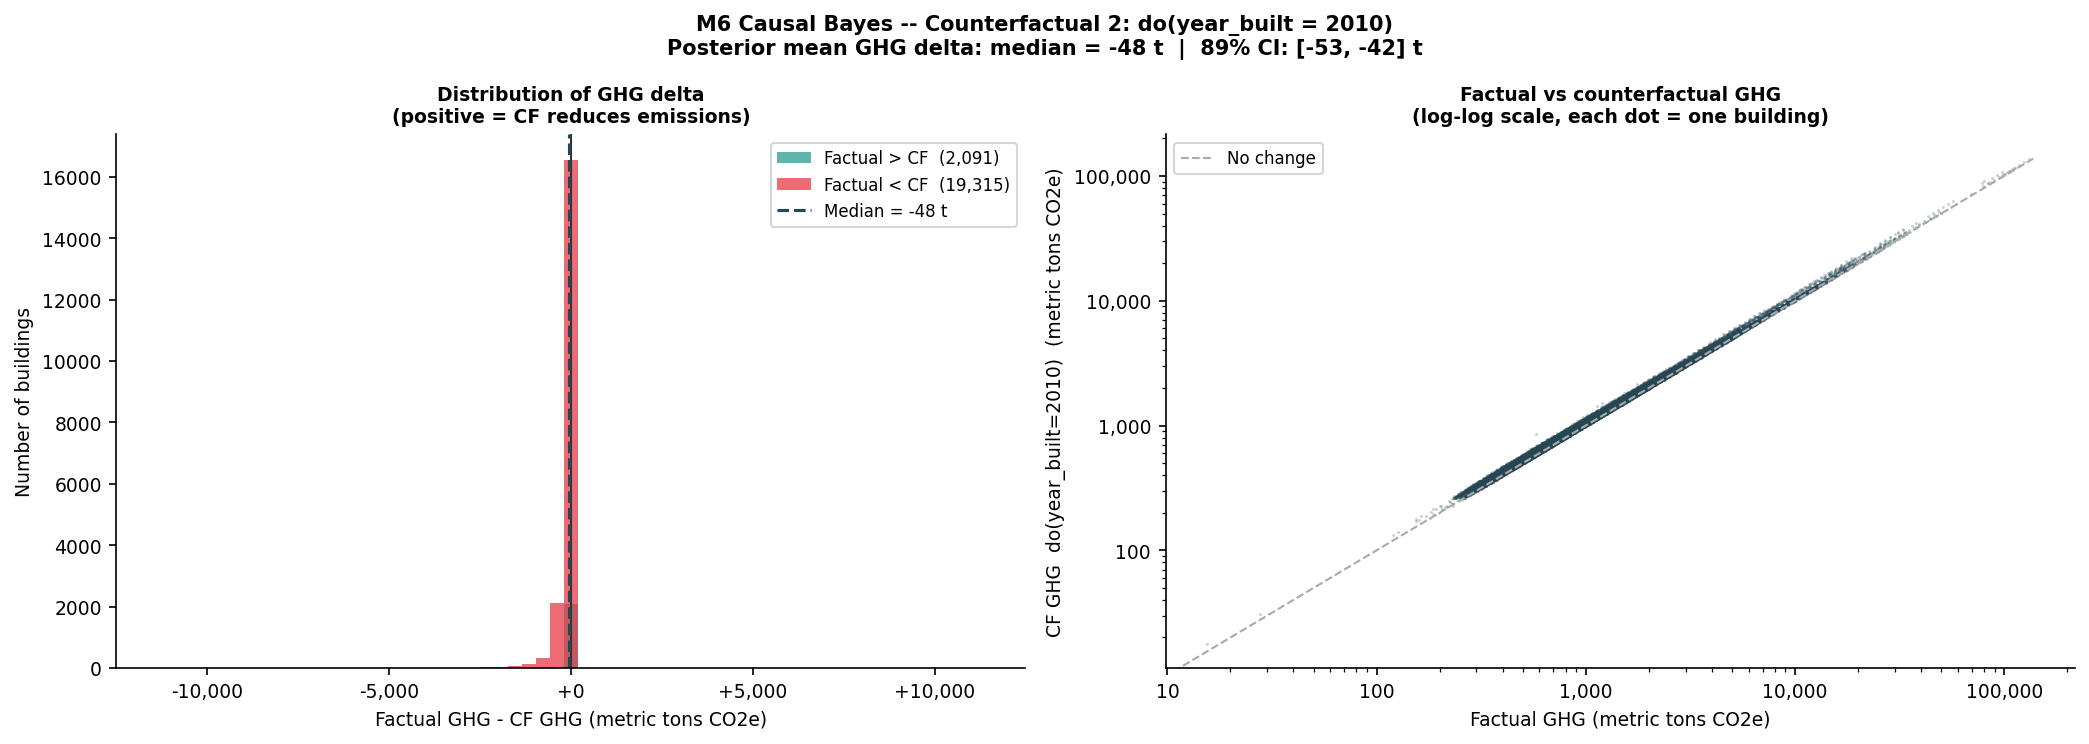
\includegraphics[width=0.95\linewidth]{figures/fig_cf2_reduction.png}
\caption*{\textbf{Figure 7.3. Vintage reassignment counterfactual.} Left: distribution of the per-record mean difference $\Delta_i$ under the 2010 reassignment, with the median marked; negative values mean the counterfactual vintage is predicted to emit more. Right: factual against counterfactual predicted GHG per record on log-log axes, where points below the diagonal would indicate a reduction. Author's analysis of Chicago Energy Benchmarking data.}
\end{figure}

The two counterfactual queries close the ladder the paper set out to climb: seeing in the shadow matrix and the associational models, doing in the inverse-probability correction, imagining in the counterfactuals of this section (\cit{pearl2009}{Pearl, 2009}). The vintage query is the sharper demonstration of why the climb matters. Its computation would have been equally possible on an asserted graph, but its counterintuitive answer would then have been indistinguishable from a specification artefact; on the tested structure, the answer has a warrant, because the separation of trend from cohort that produces it is carried by the structure that survived Stage 3.


\FloatBarrier
\section{Conclusion}

This paper began from the observation that the binding constraint in applied causal inference is not estimation but the graph: every tool in the Pearlian framework is conditional on a causal structure that, in most observational work, is asserted rather than tested. Its answer is a class and a procedure. Compliance-gated administrative datasets, defined by the three conditions of Section 2 (unit-level threshold selection on observables, endogeneity of the selection variable, atomic reporting), are a class for which that problem is tractable, because the document that creates the compliance obligation also fixes the structure it imposes on the data. The TDGP pipeline turns that property into a procedure: locate the gate in the missingness pattern (Stage 1), formulate the DAG from the gate, the shadow matrix, and the variable descriptions (Stage 2), and expose the hypothesis to falsification against the constitutive documents, which were held out from its construction (Stage 3).

On the Chicago Energy Benchmarking data the procedure ran end to end. Stage 3's sharpest test reconstructed the recorded outcome as the documented linear combination of the metered fuels to $R^2 = 0.9999$, leaving no role for a parent of the outcome beyond the mediators, and the surviving structure then licensed the ladder's upper rungs in turn. At the rung of intervention, the inverse-probability correction implemented the back-door adjustment the graph certified, and the 2$\times$3 factorial isolated what it contributes: on the corrected foundation, the structural Bayesian model matched the unconstrained gradient-boosted ensemble to within 0.4 percentage points of median absolute percentage error (21.4 against 21.0). The tie is the point, because of what it purchases: a floor-area elasticity of 0.979 with an interval that excludes proportional scaling, a decarbonisation trend of roughly 5.4 percent per year that survived every prior and weighting specification tested, a 22-fold emissions range across property types beyond what size, age, and reporting year explain, and uncertainty-carrying emission estimates for the 5,510 building-year records that never reported under the ordinance. At the rung of imagining, the same posterior answered counterfactual queries with outputs the point-prediction pipelines of Section 5 do not deliver: under trend continuation to 2030, 37.1 percent of records remain at high risk against a stylised compliance threshold, and reassigning every building's vintage to 2010 credibly raises predicted emissions for 90.2 percent of records, a sign the tested separation of trend from cohort makes interpretable rather than suspect.

The convergence of the two model families is a corollary, not a coincidence. \cit{breiman2001}{Breiman (2001)} framed the structural and algorithmic cultures as rivals; the factorial shows the rivalry dissolving under a specific and checkable condition, namely that the data-generating process is recoverable from institutional documentation and has survived a falsification test against it. When that condition holds, both families estimate the same population quantity and differ only in what they return: a number, or a mechanism with a number attached. When it does not hold, the algorithmic culture's caution stands, and nothing in this paper argues otherwise.

\subsection{Limitations}

\textbf{Selection ignorability is the residual the documents cannot reach.} Stage 3 tests which variables the gate keys on, and the data show that realised compliance departs from the documented rule: the propensity model classifies compliance at 95.1 percent accuracy, not 100 (Section 5.3). Wherever it departs, the correction rests on the standard assumption that no unobserved driver of compliance is correlated with the outcome given the upstream features (\cit{hernanrobins2020}{Hernán \& Robins, 2020}). The gate-fidelity and manipulation checks the pipeline affords (Sections 3.1, 5) audit this partially, but the unobserved component of selection that Section 5 carries as a limitation (management practices, voluntary retrofits, tenant behaviour) is exactly what no within-sample diagnostic can rule out.

\textbf{The correction stops at the overlap boundary.} Inverse-probability weighting recovers the population only where compliant units exist to be reweighted. Below the 50,000 square foot threshold there are none, so every statement about the never-observed region rides on the modularity of the tested equations and on the assumption that the learned upstream form is stable past the cutoff. Even within support, where the 5,510 non-reporting records sit, prediction outruns validation: the deployment inference of Section 6.4 was framed as consistency with the tested DGP, not as validation against ground truth, because for a never-reporting building no ground truth exists.

\textbf{The temporal trend is a bundle, and the projections assume its persistence.} $\beta_T$ mixes the decline in the grid emission factor with efficiency change in the stock, and any panel-wide operational shifts are absorbed into it as well, since occupancy and operational schedules are unobserved (Section 6.2). The policy comparisons of Section 7.1 inherit both qualifications: the pace that clears the city's 2040 target is a building-stock rate carried forward unchanged, not a forecast.

\textbf{The pipeline tests structure, not functional form.} Stages 1 to 3 settle which variables enter and how observation is gated; the linear world-layer form of the focal model was a downstream choice, and the factorial itself showed that form still matters when it is wrong: the causally-blind Bayesian model could not exploit its access to the mediators because a log-linear likelihood cannot represent their additive accounting identity (Section 5.6). The convergence result is therefore conditional on the chosen form being adequate for this outcome, as the predictive tie indicates it is here, and nothing in the pipeline guarantees adequacy elsewhere.

\textbf{Mechanism-level counterfactuals remain out of reach.} The energy mediators are compliance-gated, so the focal model operates on the reduced form from upstream features to outcome. Queries that act on the mediators, retrofit impact above all, are not identified by anything estimated here, a boundary Section 7.3 drew explicitly.

\textbf{The empirical evidence is one member of the class.} Section 2.4 argued the class is broad; the demonstration is a single city's programme over a single decade. Whether the pipeline ports as claimed, and whether parameters such as the near-unit elasticity generalise, are empirical questions this paper poses but cannot answer.

\subsection{Extensions}

The limitations order the research programme. The nearest extension is replication across the class: benchmarking ordinances of the same gate structure operate in other cities, differing in thresholds and stringency, so the pipeline can be re-run end to end and the structural parameters compared across programmes, turning the single-city caveat into a test of generalisation. Section 2.4 points further afield, to injury recordkeeping, toxics release reporting, and credit origination, where the constitutive documents differ in kind but the three conditions hold in the same form.

Two extensions strengthen the correction itself. Replacing the single propensity model with doubly robust estimation would let the analysis survive misspecification of either the selection or the outcome model; it would not discharge the ignorability assumption, which no estimator removes, but it would stop the correction depending on one specification being right. And modelling the mediator layer, which the data record for the (largely) compliant units, would extend the reach of the third rung: an inverse-probability-corrected upstream-to-mediator model, composed with the documented accounting identity, is exactly what a retrofit counterfactual requires, converting Section 7.3's stated boundary into a specification.

The deployment direction runs toward the regulator. The compliance-risk machinery of Section 7.2 applies unchanged to whatever threshold a performance standard specifies, and the posterior-predictive inventory of Section 6.4 replaces point-imputed emission gap-filling with estimates that state their uncertainty. A study built with a city's actual enforcement parameters would test whether the probabilistic classification earns its keep in practice.

The general claim survives the particulars. Wherever a written rule fixes which units are recorded, and that rule can be read, the DAG establishment problem admits a test, and a graph that has survived a test licenses what an asserted graph only borrows: adjustment with a warrant, extrapolation with a stated cost, and counterfactuals whose surprises are findings rather than artefacts (\cit{pearl2009}{Pearl, 2009}). The compliance gate, ordinarily a reason to distrust administrative data, is on this reading its most valuable feature, because the same institution that censors the data documents the process that generated it.

\subsection{Data and Code Availability}

The Chicago Energy Benchmarking dataset is publicly available from the City of Chicago Data Portal (\cit{citynd}{City of Chicago, n.d.}) and was retrieved through the portal's API; no data is redistributed with this paper. The analysis code implementing the TDGP pipeline, the 2$\times$3 factorial experiment, and the counterfactual queries is available from the author on request.



\clearpage
\section*{References}
\begin{description}\setlength{\itemsep}{0pt}
\item[] \hypertarget{bareinboimpearl2012}{}Bareinboim, E., \& Pearl, J. (2012). Controlling Selection Bias in Causal Inference. \textit{Proceedings of the 15th International Conference on Artificial Intelligence and Statistics (AISTATS)}, PMLR 22, 100--108.
\item[] \hypertarget{breiman2001}{}Breiman, L. (2001). Statistical Modeling: The Two Cultures. \textit{Statistical Science}, 16(3), 199--215. \url{https://doi.org/10.1214/ss/1009213726}
\item[] \hypertarget{city2013}{}City of Chicago. (2013). Municipal Code of Chicago, Chapter 18-14: Building Energy Use Benchmarking. American Legal Publishing Code Library. \url{https://codelibrary.amlegal.com/codes/chicago/latest/chicago_il/0-0-0-2685180}
\item[] \hypertarget{city2022}{}City of Chicago. (2022). \textit{2022 Chicago Climate Action Plan}. \url{https://www.chicago.gov/city/en/sites/climate-action-plan/home.html}
\item[] \hypertarget{citynd}{}City of Chicago. (n.d.). Chicago Energy Benchmarking [Dataset]. City of Chicago Data Portal. \url{https://data.cityofchicago.org/Environment-Sustainable-Development/Chicago-Energy-Benchmarking/xq83-jr8c}
\item[] \hypertarget{cityndb}{}City of Chicago. (n.d.b). Chicago Energy Rating. City of Chicago. \url{https://www.chicago.gov/city/en/progs/env/ChicagoEnergyRating.html}
\item[] \hypertarget{colehernan2008}{}Cole, S. R., \& Hernán, M. A. (2008). Constructing Inverse Probability Weights for Marginal Structural Models. \textit{American Journal of Epidemiology}, 168(6), 656--664. \url{https://doi.org/10.1093/aje/kwn164}
\item[] \hypertarget{connellyetal2016}{}Connelly, R., Playford, C. J., Gayle, V., \& Dibben, C. (2016). The role of administrative data in the big data revolution in social science research. \textit{Social Science Research}, 59, 1--12. \url{https://doi.org/10.1016/j.ssresearch.2016.04.015}
\item[] \hypertarget{facure2023}{}Facure, M. (2023). \textit{Causal Inference in Python: Applying Causal Inference in the Tech Industry}. O'Reilly Media.
\item[] \hypertarget{heckman1979}{}Heckman, J. J. (1979). Sample Selection Bias as a Specification Error. \textit{Econometrica}, 47(1), 153--161.
\item[] \hypertarget{hernanrobins2020}{}Hernán, M. A., \& Robins, J. M. (2020). \textit{Causal Inference: What If}. Chapman \& Hall/CRC.
\item[] \hypertarget{hsu2015}{}Hsu, D. (2015). Identifying key variables and interactions in statistical models of building energy consumption using regularization. \textit{Energy}, 83, 144-155. \url{https://doi.org/10.1016/j.energy.2015.02.008}
\item[] \hypertarget{kleven2016}{}Kleven, H. J. (2016). Bunching. \textit{Annual Review of Economics}, 8(1), 435--464. \url{https://doi.org/10.1146/annurev-economics-080315-015234}
\item[] \hypertarget{kontokostatull2017}{}Kontokosta, C. E., \& Tull, C. (2017). A data-driven predictive model of city-scale energy use in buildings. \textit{Applied Energy}, 197, 303-317. \url{https://doi.org/10.1016/j.apenergy.2017.04.005}
\item[] \hypertarget{leelemieux2010}{}Lee, D. S., \& Lemieux, T. (2010). Regression discontinuity designs in economics. \textit{Journal of Economic Literature}, 48(2), 281--355. \url{https://doi.org/10.1257/jel.48.2.281}
\item[] \hypertarget{liangzhang2026}{}Liang, H., \& Zhang, H. (2026). The political economy of mandatory disclosure: A literature review. \textit{China Journal of Accounting Research}, 19(2), 100486. \url{https://doi.org/10.1016/J.CJAR.2026.100486}
\item[] \hypertarget{littlerubin2002}{}Little, R. J. A., \& Rubin, D. B. (2002). \textit{Statistical Analysis with Missing Data} (2nd ed.). Wiley. ISBN 9780471183860.
\item[] \hypertarget{mengetal2017}{}Meng, T., Hsu, D., \& Han, A. (2017). Estimating energy savings from benchmarking policies in New York City. \textit{Energy}, 133, 415--423. \url{https://doi.org/10.1016/j.energy.2017.05.148}
\item[] \hypertarget{mohanpearl2021}{}Mohan, K., \& Pearl, J. (2021). Graphical models for processing missing data. \textit{Journal of the American Statistical Association}, 116(534), 1023--1037. \url{https://doi.org/10.1080/01621459.2021.1874961}
\item[] \hypertarget{osha2001}{}OSHA. (2001). \textit{Recording and Reporting Occupational Injuries and Illnesses}, 29 CFR Part 1904. U.S. Department of Labor, Occupational Safety and Health Administration. Partial exemption for employers with 10 or fewer employees: §1904.1; partially exempt industries: §1904.2.
\item[] \hypertarget{papadopouloskontokosta2019}{}Papadopoulos, S., \& Kontokosta, C. E. (2019). Grading buildings on energy performance using city benchmarking data. \textit{Applied Energy}, 233--234, 244--253. \url{https://doi.org/10.1016/j.apenergy.2018.10.053}
\item[] \hypertarget{pearl2009}{}Pearl, J. (2009). \textit{Causality: Models, Reasoning, and Inference} (2nd ed.). Cambridge University Press. ISBN 9780521895606.
\item[] \hypertarget{pearl2018}{}Pearl, J. (2018). Theoretical Impediments to Machine Learning With Seven Sparks from the Causal Revolution. \textit{Proceedings of the Eleventh ACM International Conference on Web Search and Data Mining (WSDM '18)}. \url{https://doi.org/10.1145/3159652.3176182}
\item[] \hypertarget{pearl2019}{}Pearl, J. (2019). The Seven Tools of Causal Inference, with Reflections on Machine Learning. \textit{Communications of the ACM}, 62(3), 54--60. \url{https://doi.org/10.1145/3241036}
\item[] \hypertarget{pearletal2016}{}Pearl, J., Glymour, M., \& Jewell, N. P. (2016). \textit{Causal Inference in Statistics: A Primer}. Wiley. ISBN 9781119186847.
\item[] \hypertarget{pearlmackenzie2018}{}Pearl, J., \& Mackenzie, D. (2018). \textit{The Book of Why: The New Science of Cause and Effect}. Basic Books.
\item[] \hypertarget{rosenbaumrubin1983}{}Rosenbaum, P. R., \& Rubin, D. B. (1983). The Central Role of the Propensity Score in Observational Studies for Causal Effects. \textit{Biometrika}, 70(1), 41--55. \url{https://doi.org/10.1093/biomet/70.1.41}
\item[] \hypertarget{rubin1976}{}Rubin, D. B. (1976). Inference and missing data. \textit{Biometrika}, 63(3), 581--592.
\item[] \hypertarget{shpitserpearl2008}{}Shpitser, I., \& Pearl, J. (2008). Complete Identification Methods for the Causal Hierarchy. \textit{Journal of Machine Learning Research}, 9, 1941--1979.
\item[] \hypertarget{departmentnd}{}U.S. Department of Labor, Occupational Safety and Health Administration. (n.d.). OSHA's Recordkeeping Requirements. Retrieved May 24, 2026, from \url{https://www.osha.gov/recordkeeping}
\item[] \hypertarget{environmentalnd}{}U.S. Environmental Protection Agency. (n.d.). Toxics Release Inventory (TRI) Program. Retrieved May 24, 2026, from \url{https://www.epa.gov/toxics-release-inventory-tri-program}
\item[] \hypertarget{epa2025}{}U.S. EPA. (2025). ENERGY STAR Portfolio Manager Technical Reference: Greenhouse Gas Emissions (August 2025). \url{https://portfoliomanager.energystar.gov/pdf/reference/Emissions.pdf}
\item[] U.S. EPA. \textit{Toxic Chemical Release Reporting: Community Right-to-Know}, 40 CFR Part 372, implementing Section 313 of the Emergency Planning and Community Right-to-Know Act (EPCRA), 42 U.S.C. §11023. Covered facilities (10 or more full-time employees): §372.22; reporting thresholds (25,000 lb manufactured or processed, 10,000 lb otherwise used): §372.25.
\item[] U.S. Securities and Exchange Commission. \textit{Definitions}, Securities Exchange Act of 1934, Rule 12b-2, 17 CFR §240.12b-2. Accelerated filer: public float of \$75 million or more (but less than \$700 million).
\item[] \hypertarget{securitiesnd}{}U.S. Securities and Exchange Commission. (n.d.). Exchange Act Reporting and Registration. Retrieved May 27, 2026, from \url{https://www.sec.gov/resources-small-businesses/going-public/exchange-act-reporting-registration}
\item[] \hypertarget{vehtarietal2017}{}Vehtari, A., Gelman, A., \& Gabry, J. (2017). Practical Bayesian model evaluation using leave-one-out cross-validation and WAIC. \textit{Statistics and Computing}, 27, 1413--1432. \url{https://doi.org/10.1007/s11222-016-9696-4}
\item[] \hypertarget{vehtarietal2021}{}Vehtari, A., Gelman, A., Simpson, D., Carpenter, B., \& Bürkner, P.-C. (2021). Rank-normalization, folding, and localization: An improved $\hat{R}$ for assessing convergence of MCMC (with discussion). \textit{Bayesian Analysis}, 16(2), 667--718. \url{https://doi.org/10.1214/20-BA1221}
\end{description}


\end{document}
